%
% Modified by Megan Patnott
% Last Change: Jan 18, 2013
%
%%%%%%%%%%%%%%%%%%%%%%%%%%%%%%%%%%%%%%%%%%%%%%%%%%%%%%%%%%%%%%%%%%%%%%%%
%
% Modified version of the sample_ndthesis.tex
% by Sameer Vijay
% Last Change: Wed Jul 27 2005 14:00 CEST
%
%%%%%%%%%%%%%%%%%%%%%%%%%%%%%%%%%%%%%%%%%%%%%%%%%%%%%%%%%%%%%%%%%%%%%%%%
%
% Sample Notre Dame Thesis/Dissertation
% Using Donald Peterson's ndthesis classfile
%
% Written by Jeff Squyres and Don Peterson
%
% Provided by the Information Technology Committee ofs
%   the Graduate Student Union
%   http://www.gsu.nd.edu/ 
%
% Nothing in this document is serious except the format.  :-)%

%%%%%%%%%%%%%%%%%%%%%%%%%%%%%%%%%%%%%%%%%%%%%%%%%%%%%%%%%%%%%%%%%%%%%%%%
% This is *not* a substitute for the documentation, which is included
% as a pdf file in the standard distribution, and can be obatined from
% the dtx file in the advanced distribution.
%%%%%%%%%%%%%%%%%%%%%%%%%%%%%%%%%%%%%%%%%%%%%%%%%%%%%%%%%%%%%%%%%%%%%%%%
%
% You should *also* have a ND formatting guide to ensure that you have
% all the relevant parts, put the captions in the right place, etc.
% Just because you have this wonderful style classfile doesn't mean
% that it removes *all* the formatting onus from you.  :-)
% Although be warned that the Graduate School has been known to let
% their official formatting guide get out of date. When in doubt,
% the Microsoft Word example seemed to be the only thing kept
% consistently up-to-date in 2013, and is probably the safest thing
% to consult.
%
% You should break all of this stuff up into separate files
% (at the very least, one chapter per file) and use the \include
% command, as has been done here for chapters 1 and 2 and the appendix.
% There is also an \input command, but \include is more commonly used to
% import chapters in books and dissertations. For the differencets between these
% two commands, see, e.g., 
% http://web.science.mq.edu.au/~rdale/resources/writingnotes/latexstruct.html
% or http://tex.stackexchange.com/questions/246/when-should-i-use-input-vs-include.
%
% If you compile from the command line, note that you should also have 
% a good Makefile; one that invokes LaTeX as many times as necessary 
% (up to 4) and bibtex if necessary.
%
% If you use an editor that allows you to compile from within the
% program, note that you will need to compile up to four times. Also,
% we recommend that you use pdflatex (sometimes displayed as
% LaTeX => PDF) to compile directly to pdf.
%
% If you have any suggestions, comments, questions, please send e-mail
% to: dteditor@nd.edu
%
%%%%%%%%%%%%%%%%%%%%%%%%%%%%%%%%%%%%%%%%%%%%%%%%%%%%%%%%%%%%%%%%%%%%%%%%

\documentclass[final,numrefs,sort&compress,noinfo]{nddiss2e}
% One of the options draft, review, final must be chosen.
% One of the options textrefs or numrefs should be chosen
% to specify if you want numerical or ``author-date''
% style citations.
% Other available options are:
% 10pt/11pt/12pt (available with draft only)
% twoadvisors
% noinfo (should be used when you compile the final time
%         for formal submission)
% sort (sorts multiple citations in the order that they're
%       listed in the bibliography)
% compress (compresses numerical citations, e.g. [1,2,3]
%           becomes [1-3]; has no effect when used with
%           the textrefs option)
% sort&compress (sorts and compresses numerical citations;
%           is identical to sort when used with textrefs)

\usepackage{multirow}
\usepackage{subfigure}
\usepackage{hyperref}
\usepackage{slashed}
%\usepackage{cite}
\usepackage{subfigure}
\usepackage{amsmath}
\usepackage{amssymb}
\usepackage{hepnicenames}
\usepackage{longtable}
\begin{document}
\providecommand{\mt}{\ensuremath{M_\mathrm{T}}\xspace}
\newcommand{\Htt}{\ensuremath{\mathrm{H} \to \tau \tau}\xspace}
\newcommand{\ETmiss}{\ensuremath{\mathrm{E}_{T}^{miss}}\xspace}
\newcommand{\Htetmu}{\ensuremath{\mathrm{H} \to \tau_{e} \tau_{\mu}}\xspace}
\newcommand{\Hteth}{\ensuremath{\mathrm{H} \to \tau_{e} \tau_{\textrm{h}}}\xspace}
\newcommand{\Het}{\ensuremath{\mathrm{H} \to e \tau}\xspace}
\newcommand{\Hmt}{\ensuremath{\mathrm{H} \to \mu \tau}\xspace}
\newcommand{\Hmue}{\ensuremath{\mathrm{H} \to \mu \tau_{e}}\xspace}
\newcommand{\Hmuhad}{\ensuremath{\mathrm{H}\to \mu\tau_{h}}\xspace}
%\newcommand\Hmuhad      {\ensuremath{\PH \to \Pgm \Pgt_{h}}\xspace}
\newcommand{\Hehad}{\ensuremath{\mathrm{H} \to e \tau_{h}}\xspace}
\newcommand{\Hemu}{\ensuremath{\mathrm{H} \to e \tau_{\mu}}\xspace}
\newcommand{\mue}{\ensuremath{\mu \tau_{e}}\xspace}
\newcommand{\emu}{\ensuremath{e \tau_{\mu}}\xspace}
\newcommand{\muhad}{\ensuremath{\mu \tau_{h}}\xspace}
\newcommand{\ehad}{\ensuremath{e \tau_{h}}\xspace}
\newcommand{\met}{\ensuremath{\cancel{\it{E}}_{T}}\xspace}
\newcommand{\mcol}{\ensuremath{M_{col}}\xspace}
\newcommand{\mvis}{\ensuremath{M_{vis}}\xspace}
\newcommand{\msig}{\ensuremath{100\:\GeV< M_{collinear} < \: 150\:\GeV}\xspace}
\newcommand{\tauh}{\ensuremath{\tau_{h}}\xspace}
\newcommand{\wjets}{\ensuremath{W+\textrm{jets}}\xspace}
\newcommand{\zjets}{\ensuremath{Z+\textrm{jets}}\xspace}



 
\frontmatter % All the items before the first chapter go in ``frontmatter''

% Titles may be 1-4 lines long. If your title is longer than 4 lines,
% the class file may have difficulty formatting the title page.
% Line-breaks in the title have to be protected with `\protect`.
\title{Search for lepton flavor violating decays of the Higgs boson}
\author{Fanbo Meng}
\work{Dissertation} % or \work{Thesis}
\degaward{Doctor of Philosophy}
\advisor{Colin Jessop}
\department{Physics}

\maketitle
%%%%%%%%%%%%%%%%%%%%%%%%%%%%%%%%%%%%%%%%%%%%%%%%%%%%%%%%%%%%%%%%%%%%%%%%
%
% Front stuff
%
%%%%%%%%%%%%%%%%%%%%%%%%%%%%%%%%%%%%%%%%%%%%%%%%%%%%%%%%%%%%%%%%%%%%%%%%

% You must either set the copyright information or put your work in the public domain.
\copyrightholder{Fanbo Meng} % See template or documentation for
\copyrightyear{2017}           % other copyright options.
%\copyrightlicense{CC-BY-4.0}
\makecopyright

% An abstract is optional for a mster's thesis, and required for a doctoral dissertation.
\begin{abstract}

A search for lepton flavour violation Higgs decay in the $H \to \mu\tau_{h}$ and $H\to e\tau_{h}$ in which tau leptons decay hadronically is presented. The search of tau lepton hadronic decay channels and the searches that are combined with tau lepton leptonic decays are presented. The $H \to e \tau_{h}$ search utilizes the 2012 proton-proton collision dataset at LHC with an integrated luminosity of 19.7 $fb^{-1}$ at a center-of-mass energy of 8 TeV collected by CMS experiment. No significant excess was observed. The upper limits on branching fraction and the corresponding Yukawa coupling were set at 95\% CL. For the $\Hmuhad$ search, the full 2016 proton-proton collision dataset with an integrated luminosity of 35.9 $fb^{-1}$ at a center-of-mass energy of 13 TeV was used. No significant excess was observed and the upper limits on branching fraction $H\to \mu\tau$ and the corresponding Yukawa coupling were set. 




\end{abstract}

% A dedication is optional.
%\renewcommand{\dedicationname}{TO MY FAMILY}

\begin{dedication}
To my family 
\end{dedication}

% These are required, and must be in this order.
\tableofcontents
\listoffigures
\listoftables

% A preface is optional.
%\begin{preface}
%probably I will write some preface, but it depends   \Hmuhad
%\end{preface}

% It's hard to tell from the information available from the Graduate
% School in Spring 2013 whether or not an acknowledgements section is optional.


\begin{acknowledge}

First I would like to thank my adviser Prof.Colin Jessop for the constant guidance, help and support in the past years in both research and everyday life. Thanks for Colin's advises step by step towards being a qualified researcher and great helps and understanding when I was in difficulties. I would also like to thank the help and accompanies from my friends at Notre Dame and CERN. Thanks for making my life colorful. Thanks for the high energy group providing me the opportunity of working at CERN. The CMS is a great collaboration with the best research environment, researchers and collaborators. 

Finally I would like to thank the love and supports from my family.  

 


\end{acknowledge}


\mainmatter



\chapter{Introduction}

The goal of elementary particle physics is to understand the fundamental particles and the interactions among them. Based in the microscopic world, particle physics attempts to construct theories that try to understand phenomena, make predictions and finally come to a consistent and unified theory. 

The Standard Model(SM) provides the modern understanding of particle physics. It incorporates the knowledge from decades of research. Except for gravity, the SM describes interactions among elementary particles that includes three out of four fundamental forces. The last missing piece, predicted by the SM, the Higgs boson was discovered in the Large Hadron Collider by both of the general purpose detectors, the CMS and ATLAS detector in 2012. The Higgs boson is a unique and crucial component of the SM. The Higgs boson is incorporated in the SM through the Higgs mechanism, which provides masses to fermions while keeping the theory renormalizable under local gauge symmetry. If viewing the Higgs mechanism within a bigger picture, the spontaneous symmetry breaking of SU(2) group, it is also related to providing the masses to other gauge bosons that mediate the interactions. The discovery of the Higgs boson is a great achievement both theoretically and experimentally. Further studies about the properties of the newly discovered boson show good agreement with the predictions from the SM. Besides the great success of the SM, there are still a number of questions that beyond the scope of the SM, for example, failing to include gravity and describing dark matter that shows its signature in the astronomy observations. New physics models are needed to understand these questions beyond the SM.  

The newly discovered Higgs boson can be a great probe to the physics beyond the SM, which in turn can test and inspire new physics models. In the SM, each flavour of leptons in the three generations is assigned a unique lepton number that is conserved within each family. The violation of this conservation which is referred as lepton flavour violation(LFV) is forbidden in the SM but allowed in many new physics scenarios. Thus, any observation of LFV will be a clear signature of new physics. The discovery of the Higgs boson can open a new window towards this topic. Before LHC era, direct searches for LFV Higgs decay, for example $H \to \mu\tau$ instead of the SM process $H \to \tau\tau$ or $H \to \mu\mu$, was impossible. The upper limits on $B(H \to \mu \tau)$ and $B(H \to e \tau)$ of $O(10\%)$~\cite{Blankenburg:2012ex,Harnik2012pb} from the indirect searches like $\tau \to \mu$ and $\tau \to e$~\cite{Celis:2013xja}. In these indirect searches, the LFV Higgs decays can only occur in the processes involving loop diagrams and the LFV Higgs decays to $\mu\tau$ and $e\tau$ from indirect searches leave plenty of room to further probe this topic. While for $H \to e\mu$, there is already a strong constrain from $\mu \to e\gamma$ at $B(H\to e \mu)<O(10^{-9})$~\cite{TheMEG2016wtm}. The CMS experiment published the first direct search on $H \to \mu \tau$ with integrated luminosity of $19.7~ fb^{-1}$ at center-of-mass energy of 8 TeV. A 2.4 $\sigma$ excess was observed and the best fit branching ratio was found to be $B(\Hmuhad)=(0.84^{+0.39}_{-0.37})\%$ at 95\% CL~\cite{2015337}. A following up search from ATLAS experiment showed the upper limits in $H \to \mu \tau$ channel as $B(H \to \mu \tau)=(1.24^{+0.50}_{-0.35})\%$ at 95\% CL~\cite{Aad2015gha}.
  

This dissertation focuses on the first direct search in $\Hehad$ with integrated luminosity of $19.7 ~fb^{-1}$ at 8 TeV and the search in $\Hmuhad$ with integrated luminosity of $35.9~ fb^{-1}$ at 13 TeV with the CMS detector. The dissertation is organized as following. A brief summary of the SM, specifically the electro-weak sector, the Higgs mechanism and LFV in beyond the SM theories are presented in Chapter 2. Following the theory chapter is the one that describes LHC and CMS experiment in general and sub-detectors in CMS. Chapter 4 includes the information about datasets used in the analyses, which incorporate the data collected from the experiment and Monte Carlo(MC) simulations, also the re-construction procedure of the basic objects used in the analysis, like muon, tau and jet. The selections used in $\Hmuhad$ and $\Hehad$ analysis are described in Chapter 5. In Chapter 6, a detailed description of the background processes considered in analyses is presented.  In chapter 7, the event selection and signal  extraction is described. In Chapter 8, the results from $\Hmuhad$ and $\Hehad$ analysis are summarized and presented. In chapter 9, the results are interpreted in terms of LFV Yukawa couplings.








%
% Chapter 2
%


\chapter{Theory}

\section{Standard model}

Standard model(SM) describes the properties of the fundamental particles currently known in the universe and the interactions amount them.  The discovery of Higgs boson in 2012 implement the last missing piece in SM.  The particles in SM is shown in Figure.~\ref{fig:SM_particles}. Besides Higgs boson, there are three generations of leptons and quarks and four gauge bosons. 
Leptons and quarks are fermions that compose the matters currently known in the universe, while the gauge bosons serve as the mediators of interactions.  

SM is a gauge theory, which describes three natural force, the strong, electromagnetic and weak force by symmetry group $SU(3)_{C}\times SU(2)_{L}\times U(1)_{Y}$. Electroweak section is described by $SU(2)_{L}\times U(1)_{Y}$. The L in $SU(2)_{L}$ stands for the left chiral signature of the weak interaction and the Y in $U(1)_{Y}$ stands for the weak hypercharge. Strong interaction is described by $SU(3)_{C}$, in which the C stands for the colors of quarks.  Photons, gluons and $W^{\pm}$, Z bosons are the mediators of electromagnetic, strong and weak force respectively.  Gravity force is not included in SM. Each particles in Figure.~\ref{fig:SM_particles} has its anti-particle or the anti-particle is the particle itself. The force and mediators characters are summarized in Table.~\ref{Mediator_infor}

\begin{figure}[htbp] 
\centering
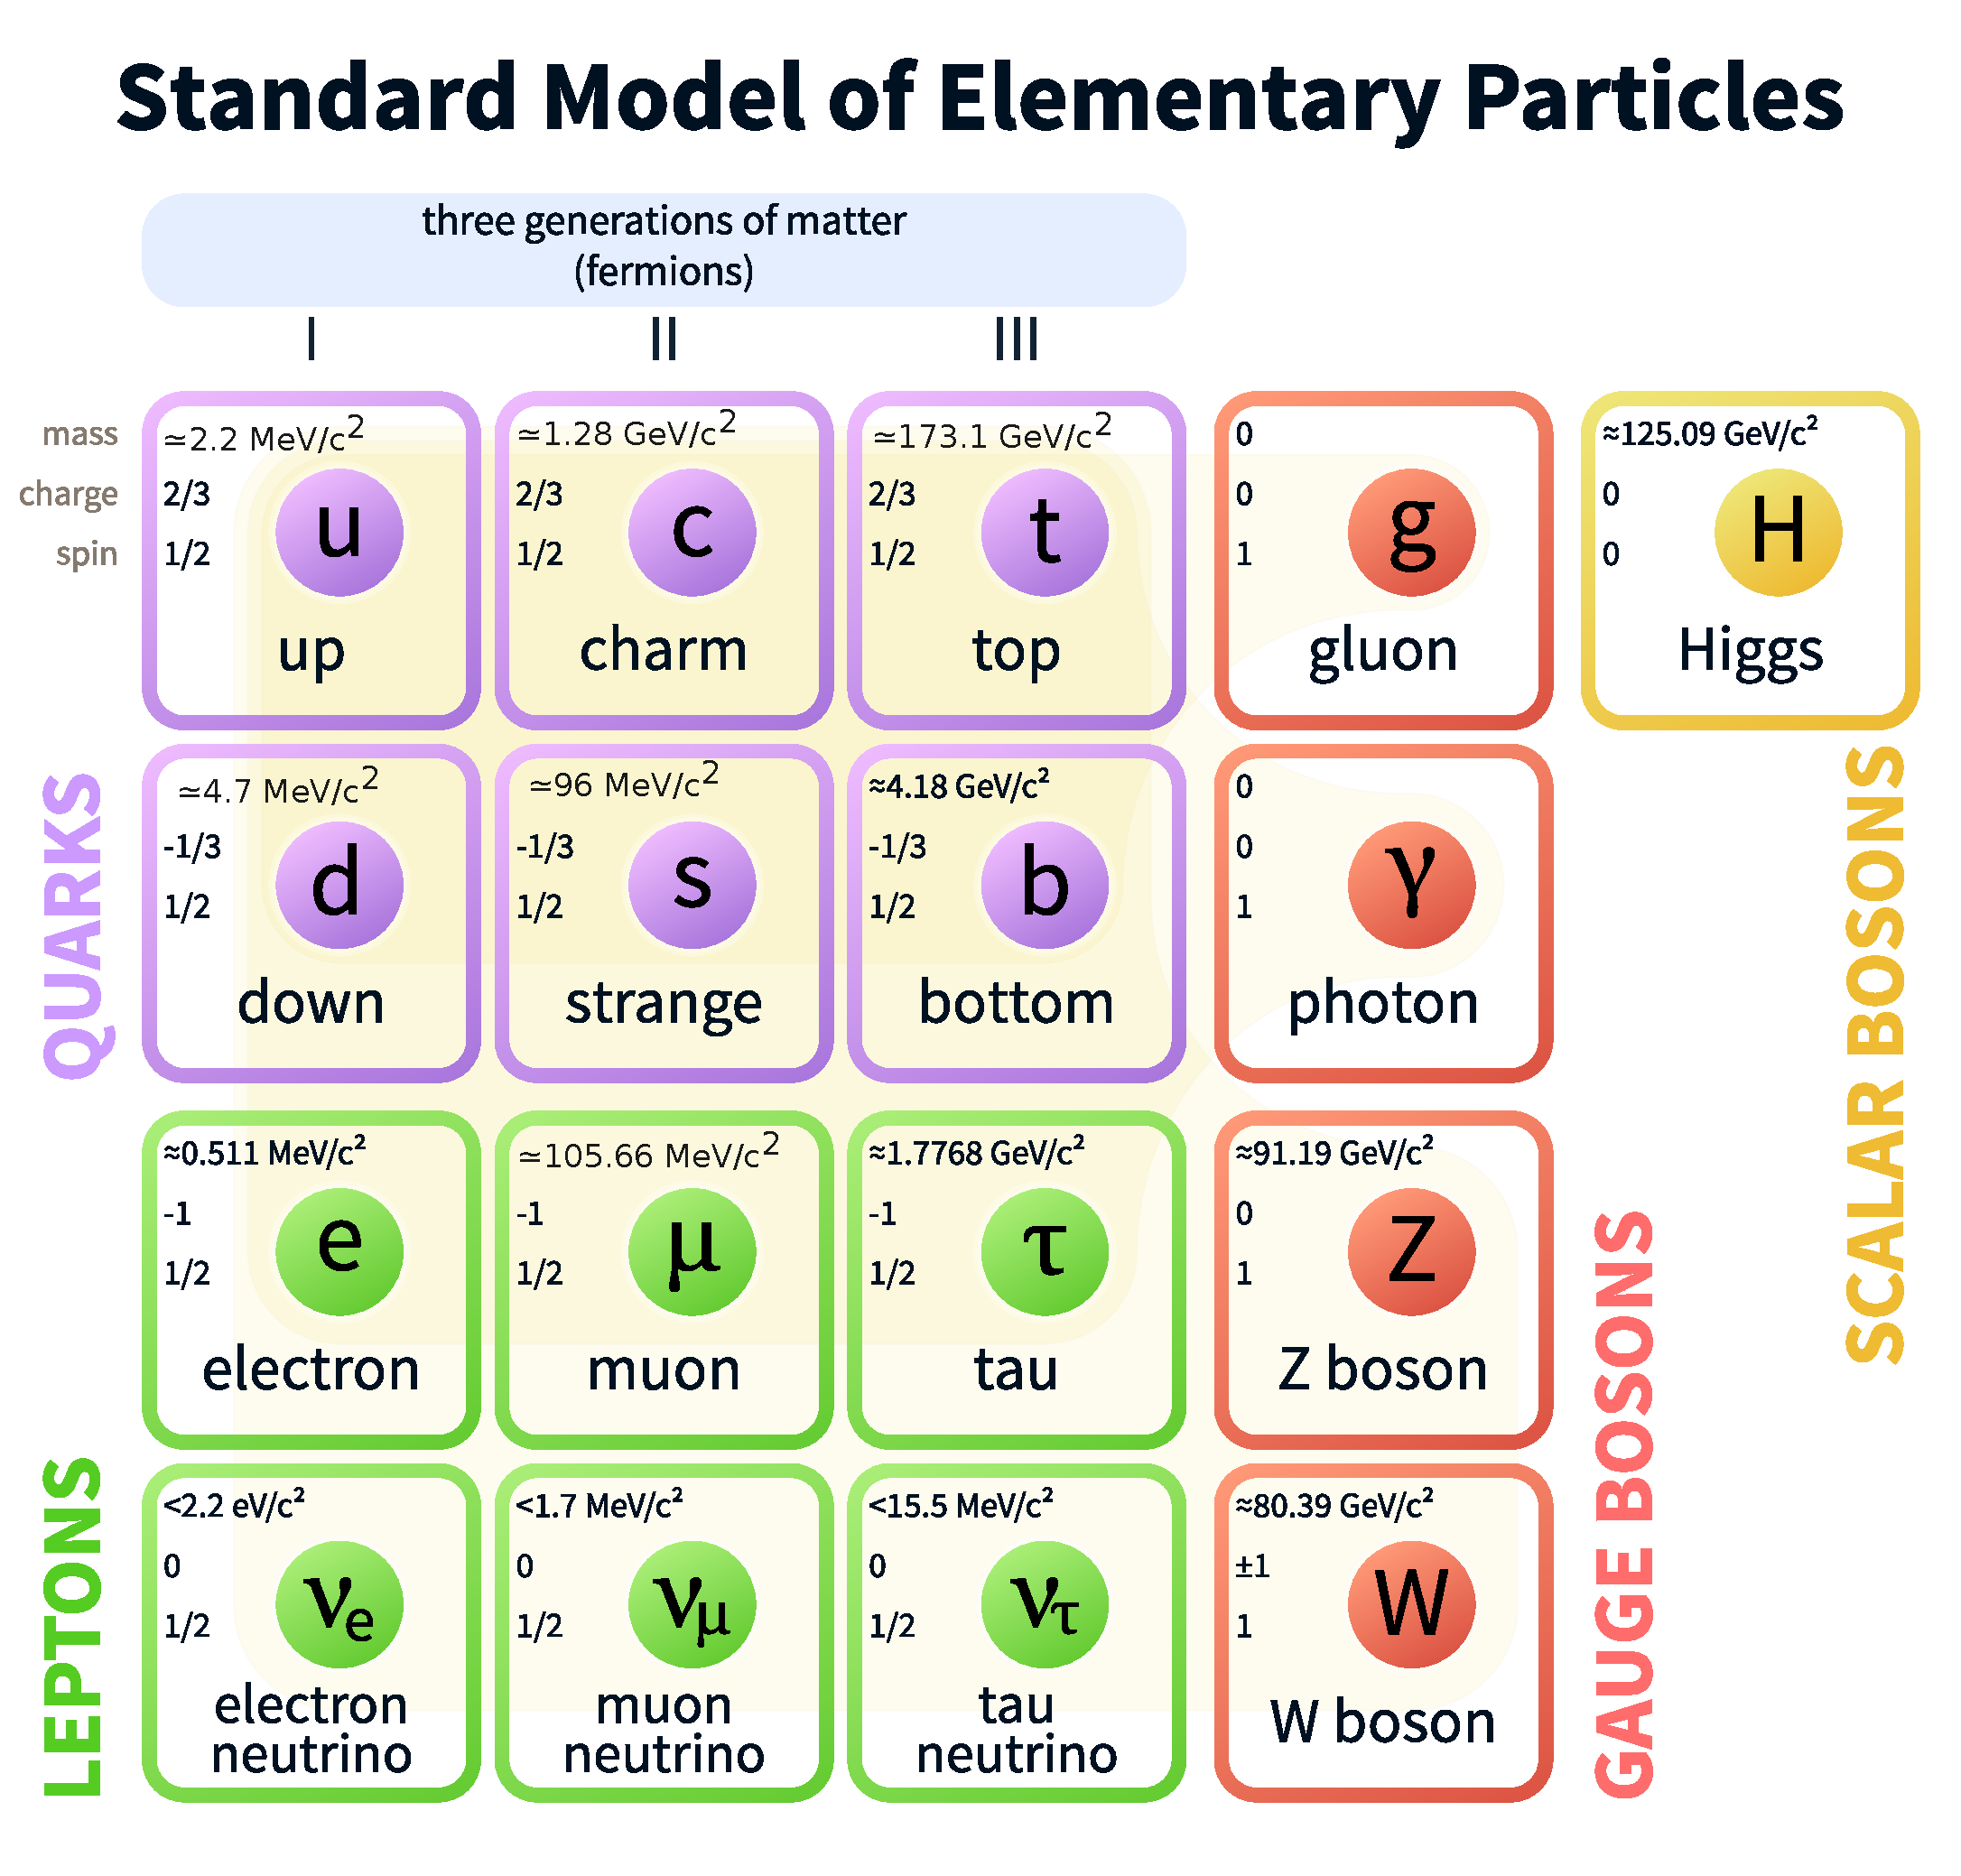
\includegraphics[width=0.8\textwidth]{chapter2/SM_particle_table.pdf}
\caption{Standard model particle group\cite{SM_particletable}}
\label{fig:SM_particles}
\end{figure}


\begin{table}[htp]
\caption{Mediators in standard model~\cite{Griffiths:111880}}
\begin{center}
\begin{tabular}{|c|c|c|c|c|}
\hline
Force & Mediator & Charge & Mass(GeV) & Range(m)   \\\hline
Strong                & g(8 gluons)                  & 0 & 0 & $10^{-15}$   \\\hline
Electromagnetic & $\gamma$(photon)     & 0 & 0 &   $\infty$   \\\hline
Weak                  &  $W^{\pm}$                &$\pm$1 & 80.379 &$10^{-18}$\\
                           & Z                                &  0         & 91.1876 &  $10^{-18}$ \\\hline
\end{tabular}
\end{center}
\label{Mediator_infor}
\end{table}%


Fermion fields in SM can be further categorized. In weak interaction, left-handed fermions are isodoublets, while right-handed fermions are isosinglets. Only the left-handed fermions or right-handed anti-fermions participate in the weak interaction. Weak hypercharge is a combined quantity, which is defined by the electric charge Q the third component of the weak isospin $I^{3}_{f}$, $Y=Q-I^{3}_{f}$. Weak interaction, together with Electromagnetic interaction are best described and understood by the electro-weak theory, which is be further discussed in the next section.  Quarks are described by SU(3), which are color triplets, while leptons are color singlets.   

Mediators in the interaction are represented by the gauge boson fields. $B_{\mu}$ is associated with symmetry $U(1)_{Y}$ and the corresponds generator is Y. $W_{\mu}^{1,2,3}$ are associated to $SU(2)_{L}$ symmetry with the generator $T^{a}$(a=1,2,3). $T^{a}$ are the $2\times2$ Pauli matrices. $G_{\mu}^{1...,8}$ are associated with the $SU(3)_{c}$ symmetry and the corresponding generators are the Gell-Mann matrices.  The field strengths are expressed as 
\begin{equation}
  \begin{aligned}
G^{a}_{\mu v}&=\partial_{\mu}G^{a}_{v}-\partial_{v}G^{a}_{\mu}+g_{s}f^{abc}G^{b}_{\mu}G^{c}_{v}\\
W^{a}_{\mu v}&=\partial_{\mu}W^{a}_{v}-\partial_{v}W^{a}_{\mu}+g_{2}\epsilon^{abc}W^{b}_{\mu}W^{c}_{v}\\
B_{\mu v}       &=\partial_{\mu}B_{v}-\partial_{v}B_{\mu}
  \end{aligned}
\end{equation}
The $g_{s}$ and $g_{2}$ are the coupling constant of $SU(3)_{C}$ and $SU(2)_{L}$ respectively. With the requirement of local gauge invariable, covariant derivatives are widely used. An example of covariant derivative acting on left-handed quarks in Lagrangian is expressed as
\begin{equation}
  \begin{aligned}
D_{\mu}\psi = (\partial_{\mu}-ig_{s}T_{a}G^{a}_{\mu}-ig_{2}T_{a}W^{a}_{\mu}-ig_{1}\frac{Y_{q}}{2}B_{\mu})
  \end{aligned}
\end{equation} 


The masses of the gauge bosons in weak interaction and fermions are generated by spontaneous symmetry breaking. Fermions specifically are generated by Higgs mechanism.  If mass terms are directly added in, the local $SU(2)\times U(1)$ will be destroyed~\cite{DJOUADI20081}. Local symmetry referring to the transformations on the fields are the functions that involve space-time. In SM, the interaction between fermion fields and scaler fields are through Yukawa's interaction.  The SM in $SU(3)_{C}\times SU(2)_{L}\times U(1)_{Y}$ symmetry without the mass terms and Yukawa's interactions is given by
 \begin{equation}
  \begin{aligned}
L_{SM}=&-\frac{1}{4}G^{a}_{\mu v}G^{\mu v}_{a}-\frac{1}{4}W^{a}_{\mu v}W^{\mu v}_{a}-\frac{1}{4}B_{\mu v}B^{\mu v}+\bar{L}_{i}iD_{\mu}\gamma^{\mu}L_{i}\\
              &+\bar{e}_{R_{i}}iD_{\mu}\gamma^{\mu}e_{R_{i}}+\bar{Q}_{i}iD_{\mu}\gamma^{\mu}Q_{i}+\bar{\mu}_{R_{i}}iD_{\mu}\gamma^{\mu}\mu_{R_{i}}+\bar{R_{i}}iD_{\mu}\gamma^{\mu}d_{R_{i}}
  \end{aligned}
\end{equation} 






\subsection{Spontaneous symmetry breaking and Higgs mechanism}

In SM, the electroweak sector follows the $SU(2)_{L}\times U(1)_{Y}$, which is spontaneously broken in the $SU(2)_{L}$ part. This mechanism plays an important role in giving mass to the mediator bosons in weak interaction and introducing the Higgs boson(Higgs).  Higgs is responsible for generating the mass of the fermions in SM, while SM remains renormalizable in local symmetry. A good example of showing the concept of spontaneous symmetry breaking with the $\phi^{4}$ theory can be found in~\cite{Peskin:1995ev}.

In the real case of SM, spontaneous symmetry breaking is introduced through a scalar doublet:
\[
\phi=
\begin{pmatrix}
\phi^{+}\\
\phi^{0}
\end{pmatrix}
=\frac{1}{\sqrt{2}}
\begin{pmatrix}
\phi_{2}-i\phi_{1}\\
\phi_{4}-i\phi_{3}
\end{pmatrix}
\]
The corresponding terms of the scalar doublet in the SM Lagrangian are expressed as
\begin{equation}
L_{s}=(D^{\mu}\phi)^{\dagger}(D_{\mu}\phi)-\mu^{2}\phi^{\dagger}\phi-\lambda(\phi^{\dagger}\phi)^{2}
\end{equation}
If $\mu^{2}<0$ and $\lambda>0$, the doublet field $\phi$ will have a none zero minimum value, which is called the vacuum expectation value(vev). In SM, the vev is shown in the following Equation and measured to be 246 GeV.
\begin{equation}\label{vev}
\langle 0 | \phi | 0 \rangle   =
\begin{pmatrix}
0\\
\frac{v}{\sqrt{2}}
\end{pmatrix}
~~~\textrm{with} ~~~  v=
\bigg(-\frac{\mu^{2}}{\lambda}\bigg)^{1/2}
\end{equation}

When the SU(2) symmetry is spontaneously broken, the scalar doublet field $\phi$ can expand around vev at first order together with the Higgs field:
\begin{equation}\label{Higgs_vev_expansion}
\phi=
\begin{pmatrix}
\theta_{2}+i\theta_{1} \\
\frac{1}{\sqrt{2}}(v+H)-i\theta_{3}
\end{pmatrix}
=e^{i\theta_{a}(x)T^{a}(x)/v}
\begin{pmatrix}
0\\
\frac{1}{\sqrt{2}}(v+H)
\end{pmatrix}
\end{equation}
Taking the unitary gauge, the scalar field transforms $\phi \to e^{-i\theta_{a}(x)T^{a}(x)/v}\phi$ and takes into $(D^{\mu}\phi)^{\dagger}(D_{\mu}\phi)$:
\begin{equation}\label{Lag_scaler}
\begin{aligned}
(D^{\mu}\phi)^{\dagger}(D_{\mu}\phi)=&|(\partial_{\mu}-ig_{2}\frac{T_{a}}{2}W^{a}_{\mu}-\frac{i}{2}g_{1}B_{\mu})\phi|^{2}\\
                                                          =&\frac{1}{2}(\partial_{\mu}H)^{2}+\frac{1}{8}g^{2}_{2}(v+H)^{2}|W^{1}_{\mu}+iW^{2}_{\mu}|^{2}\\
                                                            &+\frac{1}{8}(v+H)^{2}|g_{2}W^{3}_{\mu}-g_{1}B_{\mu}|^{2}
\end{aligned}
\end{equation}
To meets the experimental observations, re-groups the gauge fields to have the $W^{\pm}$ and Z bosons: 
\begin{equation}
W^{\pm}=\frac{1}{\sqrt{2}}(W_{1}\mp iW_{2}), Z_{\mu}=\frac{g_{2}W^{3}_{\mu}-g_{1}B_{\mu}}{\sqrt{g_{2}^{2}+g^{2}_{1}}},A_{\mu}=\frac{g_{2}W^{3}_{\mu}+g_{1}B_{\mu}}{\sqrt{g_{2}^{2}+g^{2}_{1}}},
\end{equation}
From the terms in Equation~\ref{Lag_scaler} that involving the mass of $W^{\pm}$ and Z boson, these vector bosons acquire the mass as
\begin{equation}
M_{W}=\frac{1}{2}vg_{2}~~~\textrm{and}~~~M_{Z}=\frac{1}{2}v\sqrt{g^{2}_{2}+g^{2}_{1}}
\end{equation}
while the photon $A_{\mu}$ remains massless. The mixing of electromagnetic and weak interaction is often expressed in terms of Weinberg angle or weak mixing angle. The angle $\theta_{W}$ is defined as following:
\[
\begin{pmatrix}
\gamma    \\
Z^{0}
\end{pmatrix}
=
\begin{pmatrix}
cos\theta_{W}  & sin\theta_{W} \\
-sin\theta_{W}  & cos\theta_{W}
\end{pmatrix}
\begin{pmatrix}
B\\
W_{3}
\end{pmatrix}
\]
\begin{equation}
M_{Z}=\frac{M_{W}}{cos\theta_{W}}~~~ \textrm{and}~~~
cos\theta_{W}=\frac{g_{2}}{\sqrt{g_{2}^{2}+g_{1}^{2}}}
\end{equation}

The mass of the fermions can also be generated with the interaction between the scalar doublet $\phi$ and fermion fields. Taking muon as an example, the interaction term in Lagrangian and the term that give mass to muon is shown as following:
\begin{equation}\label{Higgsmuonmass}
L_{\mu}=-\lambda_{\mu}(\bar{v}_{\mu},\bar{\mu}_{L})\phi\mu_{R}
            =-\frac{1}{\sqrt{2}}\lambda_{\mu}(v+H)\bar{\mu}_{L}\mu_{R}+ \cdots
\end{equation}
The mass of muon is given as $M_{\mu}=\frac{\lambda_{\mu}v}{\sqrt{2}}$ so as very similarly the mass of other fermions. The coupling of Higgs and fermions can also be derived from Equation.~\ref{Higgsmuonmass}~\cite{DJOUADI20081}. 

The Higgs boson production modes at LHC are the gluon-gluon fusion(ggH), the vector boson fusion(VBF), the associated production with a vector boson(VH) and the production in association with a pair of top quarks($t\bar{t}H$). The Feynman diagrams for these production modes are shown in Figure.~\ref{fig:SM_H_production}. In LHC, the proton proton collision, the real collisions are between quarks and gluons. The ggH holds the biggest Higgs production cross section, while the VBF follows. The other two are relatively small compared with ggH and VBF, thus, these two main production modes are the ones considered in the analysis that talked in the later chapters.   
\begin{figure}[htbp] 
\centering
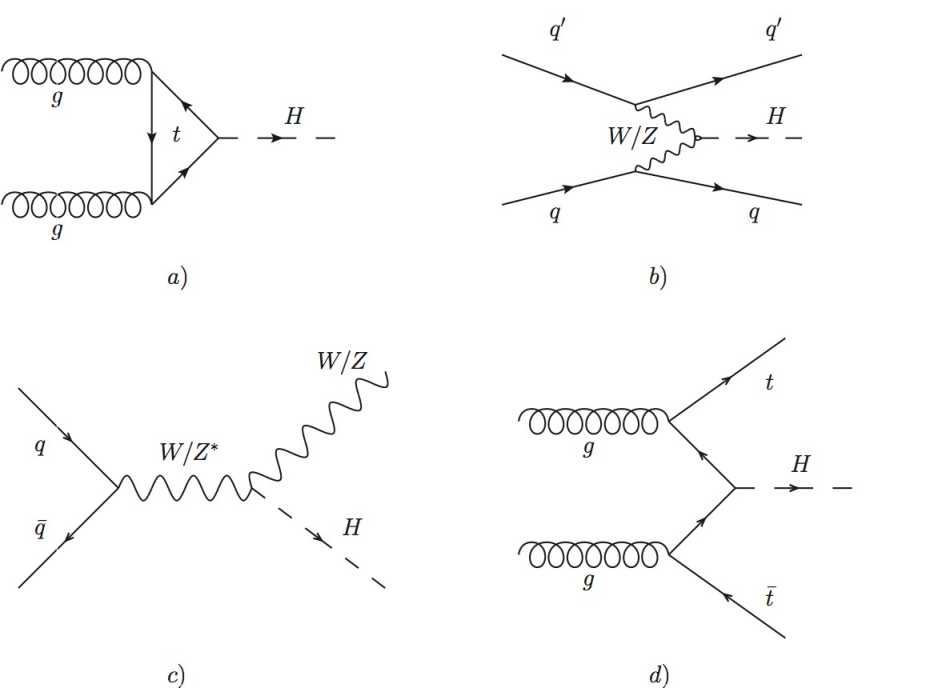
\includegraphics[width=0.8\textwidth]{chapter2/Higgs_production.jpg}
\caption{Production models in LHC}% \cite{Higgs_production_mode}}
\label{fig:SM_H_production}
\end{figure}









\section{Lepton flavour violation in beyond stand model theories}
Lepton flavour violating Higgs decays are forbidden in SM. The specific terms will not be compatible with renormalization. But beyond Standard Model, Lepton flavour conservation does not necessarily hold. In the following, two methods that can have lepton flavour violation are introduced, one model independent effective field approach and one with two Higgs doublet model. In both case, the focus is LFV Higgs decays and to show how LFV Higgs decays shows up in the new theories. 


\subsection{Lepton flavour violation Higgs decay in effective field theory}\label{effective_field}
The Effective Lagrangian approach is widely used to explore the new physics with higher dimensional operators in a model independent way. The Lagrangian in the theory can be written as following up to dimension six: 
\begin{equation}
L_{eff}=L_{SM}+\sum\frac{a^{ij}_{n}}{\Lambda^{2}}O^{ij}_{n}
\end{equation}
where $a^{ij}_{n}$ is the coefficients, $i,j,(=1,2,3)$ are flavour indices, n holds the number of the operators and $\Lambda$ is the new physics scale. 

There are various operators that can introduce processes that violate lepton flavour conservation~\cite{PhysRevD.62.116005}. As an example that most relevant to LFV Higgs decays, Yukawa-type operators that generate LFV Higgs decays only will be discussed. The Yukawa-type operators hold the following terms:
\begin{equation}
O^{ij}_{L\phi}=(\Phi^{\dagger}\Phi)(\bar{L}_{L_{i}}l_{R_{j}}\Phi)
\end{equation}
While, inside the Lagrangian, the change to SM Lagrangian takes the form:
\begin{equation}
\Delta L_{Y}=-\frac{\lambda^{'}_{ij}}{\Lambda^{2}}(\Phi^{\dagger}\Phi)(\bar{L}^{i}_{L}l^{j}_{R}\Phi)+h.c...
\end{equation}
Taking in the scalar doublet expansion around vev as shown in Equation.~\ref{Higgs_vev_expansion}, the O(6) Yukawa-type operators have the following form:
\begin{equation}
\begin{aligned}
\Delta L_{Y}=&-\frac{\lambda^{'}_{ij}}{\Lambda^{2}}(\Phi^{\dagger}\Phi)(\bar{L}^{i}_{L}l^{j}_{R}\Phi)+h.c...\\
         =&-\frac{\lambda^{'}_{ij}}{2\sqrt{2}\Lambda^{2}}l_{L}^{i}l_{R}^{j}(v+H)^{3}+h.c...\\
         =&-\frac{\lambda^{'}_{ij}v^{3}}{2\sqrt{2}\Lambda^{2}}l_{L}^{i}l_{R}^{j}-\frac{\lambda^{'}_{ij}3v^{2}}{2\sqrt{2}\Lambda^{2}}l_{L}^{i}l_{R}^{j}+h.c...
\end{aligned}
\end{equation}
The new Yukawa coupling terms have effects on fermion masses and SM Yukawa interactions. The SM components in Equation.~\ref{Higgsmuonmass} is obtained through the diagonalization of mass matrices~\cite{Harnik:2012pb}. The total Lagrangian is a combination of SM Lagrangian $L_{SM}$ and the effective field Lagrangian $\Delta L_{Y}$. Thus the combined fermion mass and Yukawa interaction terms are following:
\begin{equation}
\sqrt{2}m=V_{L}\Big[\lambda+\frac{v^{2}}{2\Lambda^{2}}\lambda^{'}\Big]V^{\dagger}_{R},~~\sqrt{2}Y=V_{L}\Big[\lambda+3\frac{v^{2}}{2\Lambda^{2}}\lambda^{'}\Big]V^{\dagger}_{R}
\end{equation}
The Yukawa couplings of Higgs and leptons mixed in the contributions from dimension six operators and have the following form, in which $\hat{\lambda=V_{L}\lambda^{'}V_{R}}$
\begin{equation}
Y_{ij}=\frac{m_{i}}{v}\delta_{ij}+\frac{v^{2}}{\sqrt{2}\Lambda^{2}}\hat{\lambda}_{ij}
\end{equation}
In the limit $\Lambda \to \infty$, the SM results can be recovered, but in general case, like in the electro-weak scale and a arbitrary non-diagonal matrix $\hat{\lambda}$, LFV Higgs decays can be introduced into the theory through effective fields.




\subsection{LFV in two Higgs models}

In the model with two Higgs doublets(2HDM) $\Phi_{1}$ and $\Phi_{2}$, similar to the SM, the Yukawa interaction can be written as: 
\begin{equation}
L=y_{1}\bar{L}\Phi_{1}E+y_{2}\bar{L}\Phi_{2}E+h.c,
\end{equation}
Here, $y_{1}$ and $y_{2}$ are Yukawa couplings. If there is not a parity symmetry distinguish the two Higgs doublets, there can be coupling of the two doublets to the leptons in the tree level. In general it is impossible to diagonalize $y_{1}$ and $y_{2}$ simultaneously and the LFV Higgs decay can be presented in the renormalizable Lagrangian~\cite{deLima2015}. A bit more description of 2HDM is in the following~\cite{BRANCO20121}.   


In 2HDM, there are in general four sub-type of models, the main difference comes from the coupling of Higgs doublets to the quarks and leptons as shown in Table.~\ref{2HDM_models}.
\begin{table}[htp!]
\caption{Four types of 2HDM models differs by the coupling to Higgs doublet fields}
\begin{center}
\begin{tabular}{|c|c|c|c|}
\hline
Model                                 &~  $u^{i}_{R}$~  &~  $d^{i}_{R}$ ~   &~   $e^{i}_{R}$ ~\\\hline
Type I                                 &  $\Phi_{2}$    &  $\Phi_{2}$     &  $\Phi_{2}$   \\\hline
Type II                                &  $\Phi_{2}$    &  $\Phi_{1}$     &  $\Phi_{1}$   \\\hline
Type III (lepton specific)     &  $\Phi_{2}$    &  $\Phi_{2}$     &  $\Phi_{1}$   \\\hline
Type IV (Flipped)                &  $\Phi_{2}$    &  $\Phi_{1}$     &  $\Phi_{2}$   \\\hline
\end{tabular}
\end{center}
\label{2HDM_models}
\end{table}
The type III 2HDM is more relevant to LFV which can have the tree level LFV Higgs decay. The Higgs doublets can have the general form:
\begin{equation}
\Phi_{j}=
\begin{pmatrix}
\phi^{+}_{j}    \\
(v_{j}+\phi_{j}+i\eta_{j}/\sqrt{2})
\end{pmatrix}
\end{equation}
Under the common assumption of CP conservation in the Higgs sector and not spontaneously broken, the quartic odd terms are eliminated in the potential, then the scalar potential can be expressed as
\begin{equation}
\begin{aligned}
V=&m^{2}_{11}\Phi^{\dagger}_{1}\Phi_{1}+m^{2}_{22}\Phi^{\dagger}_{2}\Phi_{2}-m^{2}_{12}(\Phi^{\dagger}_{1}\Phi_{2}+\Phi^{\dagger}_{2}\Phi_{1})+\frac{\lambda_{1}}{2}(\Phi^{\dagger}_{1}\Phi_{1})^{2}+\\
  &\frac{\lambda_{2}}{2}(\Phi^{\dagger}_{2}\Phi_{2})^{2}+\lambda_{3}\Phi^{\dagger}_{1}\Phi_{1}\Phi^{\dagger}_{2}\Phi_{2}+\lambda_{4}\Phi^{\dagger}_{1}\Phi_{2}\Phi^{\dagger}_{2}\Phi_{1}+\frac{\lambda_{5}}{2}[(\Phi^{\dagger}_{1}\Phi_{2})^{2}+(\Phi^{\dagger}_{2}\Phi_{1})^{2}]
  \end{aligned}
\end{equation}
The scalar doublets fields $\Phi_{1}$ and $\Phi_{2}$ are not physical observables but the mass eigenstates. So any combination of the scalar doublet fields, as long as it preserve CP and solid gauge symmetries in SM, produces the same physics results~\cite{BRANCO20121}. The following based is referred as Higgs basis for the Higgs doublets:
\begin{equation}\label{Higgs_base}
H_{1}=
\begin{pmatrix}
G^{+}    \\
\frac{1}{\sqrt(2)}(v+\phi^{0}_{1}+iG^{0})
\end{pmatrix}~,~
H_{2}=
\begin{pmatrix}
H^{+}    \\
\frac{1}{\sqrt(2)}(\phi^{0}_{2}+iA)
\end{pmatrix}
\end{equation}
The relationship between scalar field $\rho_{1}$ and $\rho_{2}$ and Higgs mass eigenstates h and H is the following:
\begin{equation}\label{Higgs_mass_states}
\begin{aligned}
h=&sin(\alpha-\beta)\phi_{1}^{0}+cos(\alpha-\beta)\phi_{2}^{0}\\
H=&cos(\alpha-\beta)\phi_{1}^{0}-sin(\alpha-\beta)\phi_{2}^{0}
\end{aligned}
\end{equation}
The angle $\alpha-\beta$ is the mixing angle between these two groups of scalars. The interactions of Higgs and fermions are through Yukawa coupling. In the Higgs base, the Yukawa interaction terms in the Lagrangian of the 2HDM can be expressed as:
\begin{equation}
\begin{aligned}
-L_{Y}=&\sqrt{2}\big(\bar{q}_{L_{j}}\tilde{H}_{1}\frac{K^{\ast}_{ij}m^{U}_{i}}{v}u_{R_{i}}+\bar{q}_{L_{i}}H_{1}\frac{m^{D}_{i}}{v}d_{R_{i}}+\bar{l}_{L_{i}}H_{1}\frac{m^{E}_{i}}{v}e_{R_{i}}\big) \\
            &+\bar{q}_{L_{i}}\tilde{H}_{2}\rho^{U}_{ij}u_{R_{j}}+\bar{q}_{L_{i}}H_{2}\rho^{D}_{ij}d_{R_{j}}+\bar{l}_{L_{i}}H_{2}\rho^{E}_{ij}e_{R_{j}}+h.c..
\end{aligned}
\end{equation}
Inside the Lagrangian, the terms denote as following, $\tilde{H}_i=i\sigma_{2}H^{\ast_{i}}$,  $K_{ij}$ as the CKM matrix and $\rho^{U,D,E}$ are complex matrices in flavor space. Taking in Equation.~\ref{Higgs_base} and \ref{Higgs_mass_states}, the lepton Yukawa interaction terms are collected as:
\begin{equation}
\begin{aligned}
-L_{Y}=&\bar{e}_{i}\big(\frac{m^{E}_{i}}{v}\delta_{ij}s_{\beta-\alpha}+\frac{1}{\sqrt{2}}\rho^{E}_{ij}c_{\beta-\alpha}\big)e_{j}h\\
            &+\bar{e}_{i}\big(\frac{m^{E}_{i}}{v}\delta_{ij}c_{\beta-\alpha}-\frac{1}{\sqrt{2}}\rho^{E}_{ij}S_{\beta-\alpha}\big)e_{j}H+...
\end{aligned}
\end{equation}
Term $s_{\beta-\alpha}$ and $c_{\beta-\alpha}$ stand for $sin_{\beta-\alpha}$ and $cos_{\beta-\alpha}$ respectively. The coupling of leptons and Higgs in the 2HDM model typeIII are expressed as
\begin{equation}
\begin{aligned}
g_{hff^{'}}&=\frac{m_{f}}{v}s_{\beta-\alpha}\delta_{ff^{'}}+\frac{\rho_{ff^{'}}}{\sqrt{2}}c_{\beta-\alpha}\\
g_{Hff^{'}}&=\frac{m_{f}}{v}s_{\beta-\alpha}\delta_{ff^{'}}-\frac{\rho_{ff^{'}}}{\sqrt{2}}c_{\beta-\alpha}\\
\end{aligned}
\end{equation}
So this shows the possibility of LFV Higgs decay at tree level~\cite{PhysRevD.90.115004}.










%
% Chapter 3
%

\chapter{LHC and CMS experiment}

Large Hadron Collider~\cite{LHC_refer} is the most powerful hadron collider ever built. The circumference of this circle superconducting collider is 26.7 km and the designed full operation energy is 14 TeV. In 2012 LHC operates on 8 TeV and in 2016, it boosts up to 13 TeV. There are four experiments hold on the LHC ring, ALICE, ATLAS, CMS and LHCb. ATLAS and CMS are general purpose detectors, aiming for the high luminosity in the order $L=10^{34} cm^{-2}s^{-1}$. LHCb focuses on the b physics study, while ALICE studies the lead-lead collision.

\section{LHC accelerator}

A sketch view of the proton accelerating process is shown in Figure.~\ref{fig:LHC_sketch}. LHC is the last and most powerful accelerator in the accelerating chain. Before the beams are injected into LHC, a series of steps are taken. For the proton-proton(p-p) collision, protons are from the source Duoplasmatron, which uses electric field to break down hydrogen gas into protons and electrons, then protons are accelerated by a 90 kV supply. Leaving the source, the protons are focused and accelerated to 750 keV by radio frequency quadrupole. Then the protons are further accelerated by linear accelerator Linac2 to 50 MeV. Proton synchrotron booster further accelerate protons from 50 MeV to 1.4 GeV and injects protons into Proton synchrotron(PS). PS accelerates protons to 25 GeV followed by the super proton synchrotron which boost the protons to 450 GeV. LHC is the last ring in the whole accelerating process and accelerate the protons to its final energy 6.5 GeV(or 7 GeV). In a normal fill with protons, LHC holds 2808 bunches with an approximation of $10^{11}$ protons.

There are thousands of superconducting magnets along the LHC ring to bend and focus the beam. Among the magnets, there are 1232 main dipoles, which are used to bend the beam with an operating field above 8 T. Other types of magnets, for example, quadrupoles magnets can tight the beam either vertically or horizontally while  sextupole, octupole and decapole can help fine tuning the magnetic field. The radiofrequency cavities(RF) in the LHC are used to accelerate the protons from 450 GeV to 6.5 GeV(or 7 GeV), keep the bunches in the beam pipe compact and store the energy loss from synchrotron radiation. Eight RFs per beam, providing 16 MV  longitudinal oscillating voltage with the 400 MHz superconducting cavity system. 

Machine luminosity is an important parameter of the collider. For a process under study, the number of events created per-second $N_{\textrm{event}}$ is shown in Equation.~\ref{event_number}, in which L is the machine luminosity and $\sigma_{event}$ is the cross section of that process.

\begin{align}\label{event_number}
N_{\textrm{event}}=L\sigma_{event}
\end{align}

Machine luminosity is determined by a number of factors as shown in Equation.~\ref{Lumi_express}. $n_b$ and $N_{b}$ are the number of bunches per-beam and the number of protons per-bunch.$f_{rev}$ and $\gamma_{\gamma}$ are the revolution frequency and relativistic gamma factor respectively. $\beta*$ is the amplitude function of the beam at the collision point while function F describes the reduction of luminosity because of the crossing angle. This machine luminosity is also called instantaneous luminosity which is the luminosity at a unite time. The integrated luminosity which later referred as luminosity is instantaneous luminosity integrating over time~\ref{fig:LHC_sketch}.  

\begin{align}\label{Lumi_express}
L=\frac{N_{b}^{2}n_{b}f_{fev}\gamma_{\gamma}}{4\pi\epsilon\beta*}F
\end{align}



\begin{figure}[htbp] 
\centering
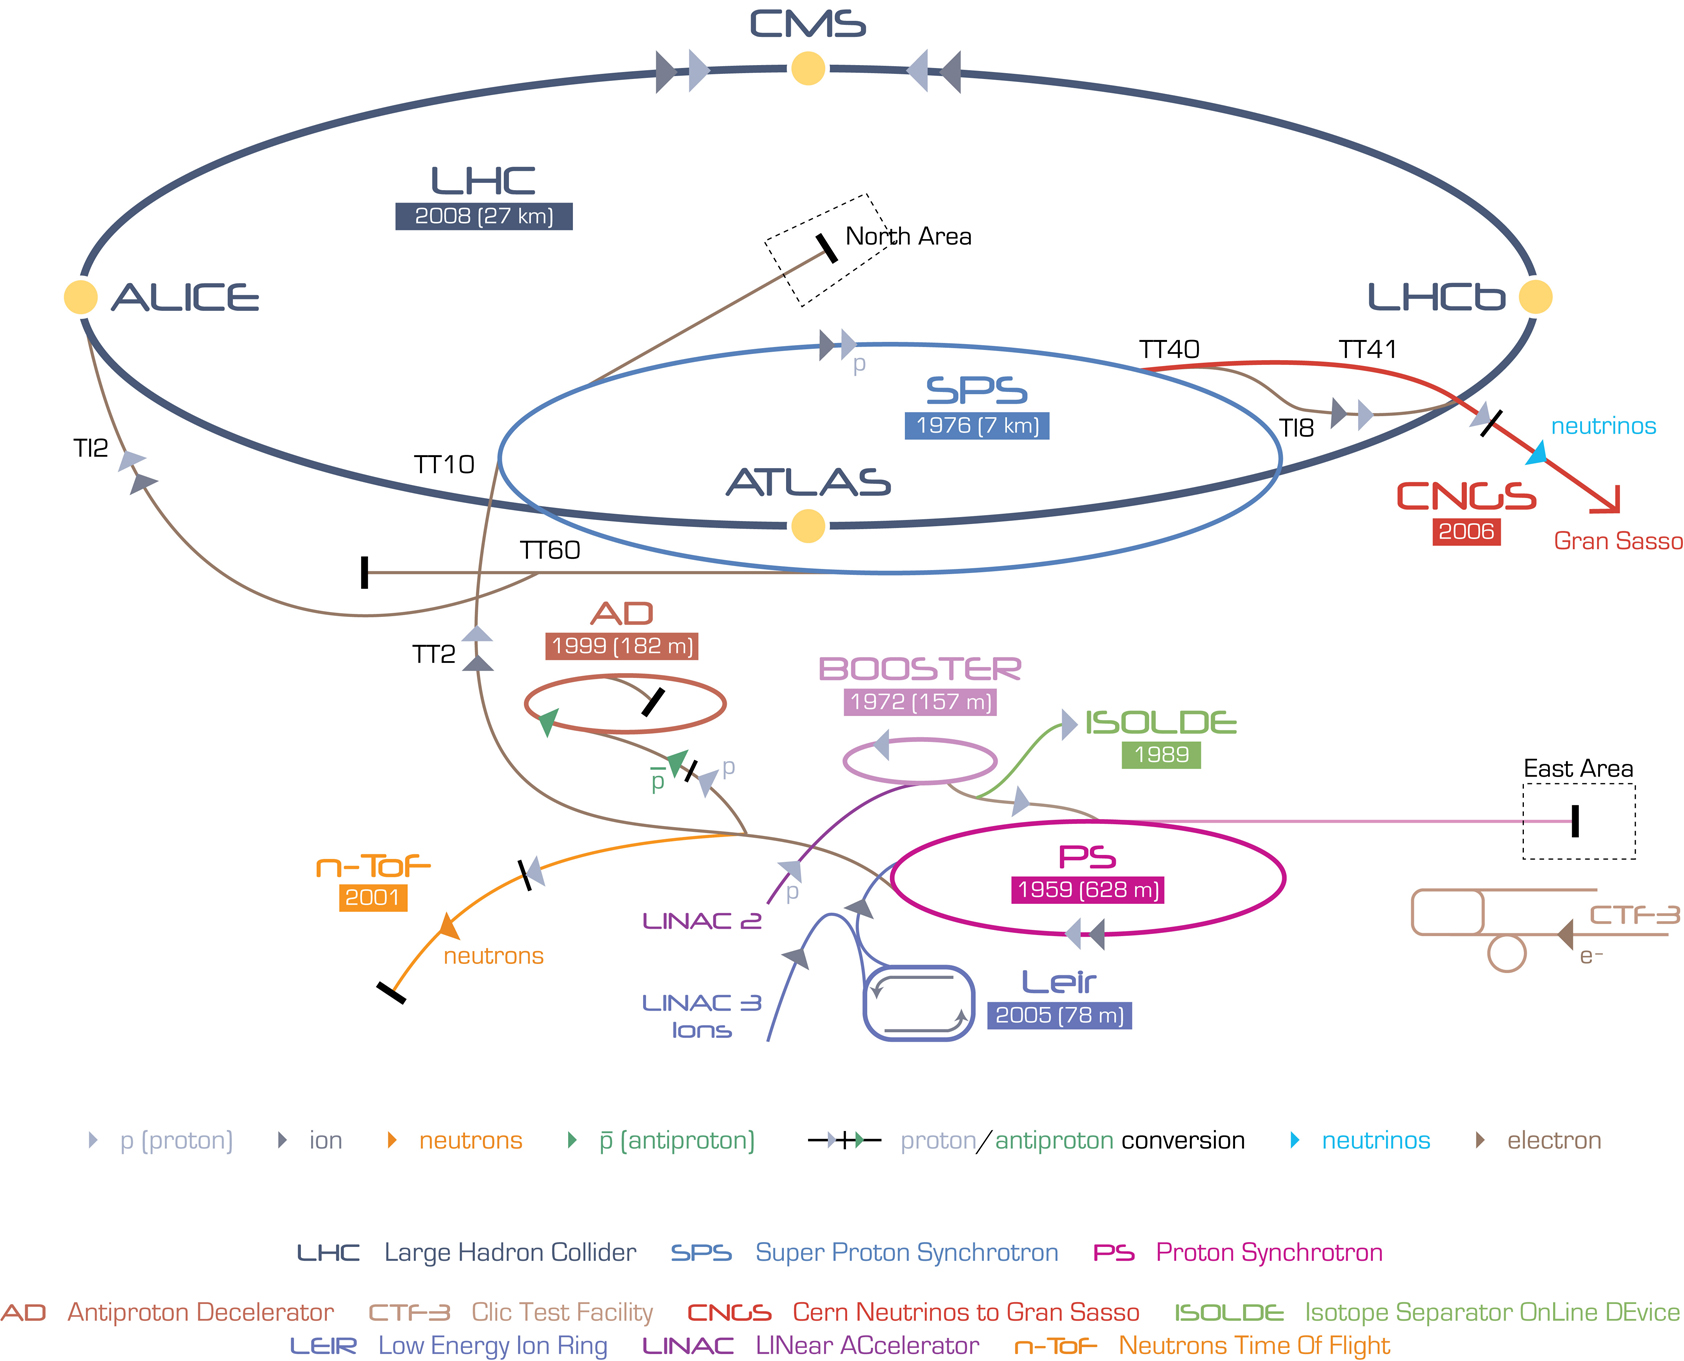
\includegraphics[width=0.8\textwidth]{chapter3/LHC_chain.jpg}
\caption{A sketch view LHC injection chain and main experiments associated~\cite{Christiane:1260465}.}
\label{fig:LHC_sketch}
\end{figure}


\section{Compact Muon Solenoid}
Compact muon solenoid(CMS) is a general purpose detector, which institutes in one of LHC collision point. It is a high performance detector that covers a broad range of physics researches, like Standard model physics, supersymmetry and dark matter. CMS detector is designed to have good muon momentum and position resolution over large range of energy and angles, good charged particle momentum resolution and high identification efficiency within inner tracker, good electromagnetic energy and position resolution and high photon and lepton isolation efficiency in high luminosity condition, good missing transverse momentum and jet energy resolution.  


An general view of CMS detector is shown in Figure.~\ref{fig:CMS_sketch}. The detector is composed of a set of sub-detectors from the inside and out in a ring structure. The main sub-detectors are the following:

\begin{figure}[htbp] 
\centering
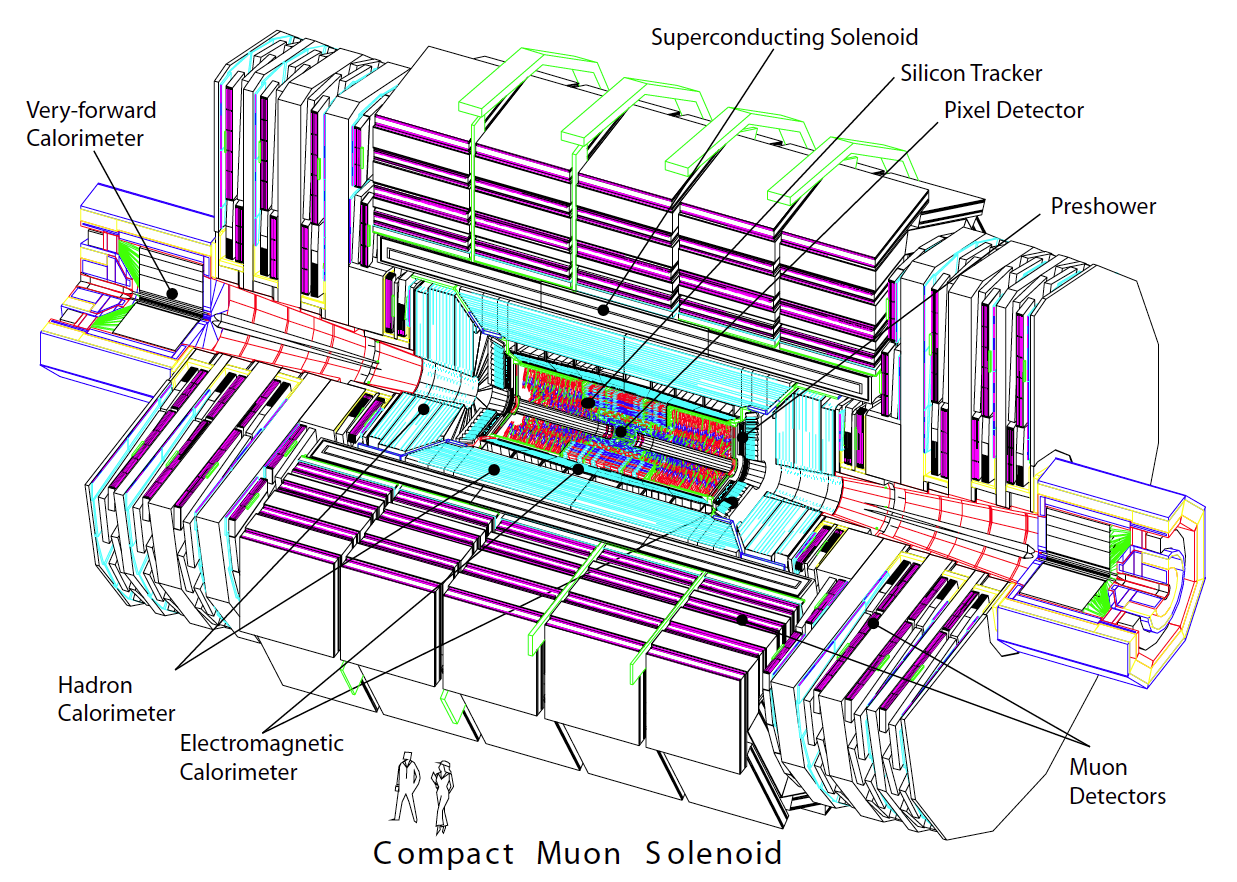
\includegraphics[width=0.8\textwidth]{chapter3/CMS_detecter.png}
\caption{A sketch view of CMS detector~\cite{CMS_experiment}}
\label{fig:CMS_sketch}
\end{figure}


\begin{enumerate}[$\bullet$]
\item Tracker consists two parts, the pixel detector and silicon tracks which are used measure the momentum and tracks of the charged particles.
\item Electromagnetic calorimeter mainly measures the energy and the position of electrons and photons. Other particles will leave some percentage of energy inside. 
\item Hadron calorimeter measures the energy of hadrons 
\item Muon detector measures the tracks and momentum of the muons.
\end{enumerate} 

Another outstanding feature of CMS is the superconducting magnet system, which provide a 3.8 T magnetic field. The configuration of the magnet system drives the design and layout of the detector. Besides the sub-detectors listed above, trigger system is also crucial for the success of the whole program. Trigger system consists two parts, the hardware based level one trigger and the software based high level trigger. Trigger system does the initial selection of interesting events from a huge flux of events per-collision, which makes it possible for data-acquisition and recording. The details of the sub-detectors and other systems mentioned will be presented later. 

In general CMS detector is 21.6 m long, 14.6 in diameter and weighted 12500 tonnes in total. The coordinate system adopted by CMS sets the center at the collision point. The x-axis points towards the center of LHC and z-axis points along the beam direction. The azimuthal angle $\phi$ is used to measure the angle from x-axis in the x-y plane and polar angle $\theta$ measures the angle from z-axis and r is the radial coordinate. Another variable called the pseudorapidity $\eta$, defined as $\eta=-\textrm{ln}\textrm{tan}(\theta/2)$ is also frequently used in the measurements. In the case $E\gg m$, pseudorapidity can be approximated as $\eta=-\textrm{ln}\big(\frac{E+p_{z}}{E-p_{z}}\big)$, where $p_{z}$ is the longitudinal component of momentum~\cite{CMS_experiment}. 

\subsection{Tracker}
The main purpose of inner tracking system of CMS is measuring the trajectories of charged particles from the LHC collision. The efficient and precise measurement is crucial for the reconstruction and identification of particles. LHC operates with the instantaneous luminosity in the order of $10^{34}cm^{-2}s^{-1}$, in average more than 20 p-p interactions and 1000 particles per-bunch crossing. High granularity and fast response is primary important for the tracker system. To measure the trajectories precisely, low interaction of tracker materials with incoming particles, like multi-scattering, photon conversion and nuclear interaction is also important. In the long operation period, radiation hardness of the tracker material is needed. All of these factors drive the design of CMS tracker system.

The tracker system of CMS surrounds the collision point with the dimension 5.8 m in length and 2.5 m in diameter, with a coverage up to pseudorapidity $|\eta|<2.5$. A overview of the tracker system layout is shown in Figure.~\ref{fig:tracker_sketch}. Three layers of silicon pixel detector modules surround the interaction points and two additional disks of pixel modules on each side, in all 66 million pixels of the size $100\times150 \mu m$ each. Following the pixel detector is the silicon strip tracker. There are four components of strip tracker, tracker Inner barrel(TIB), tracker inner Discs(TID), tracker outer barrel(TOB) and tracker end caps(TEC). The strip tracker components arrangement as shown in Figure.~\ref{fig:tracker_sketch}, consisting of about 10 million strips and 10 layers. 


\begin{figure}[htbp] 
\centering
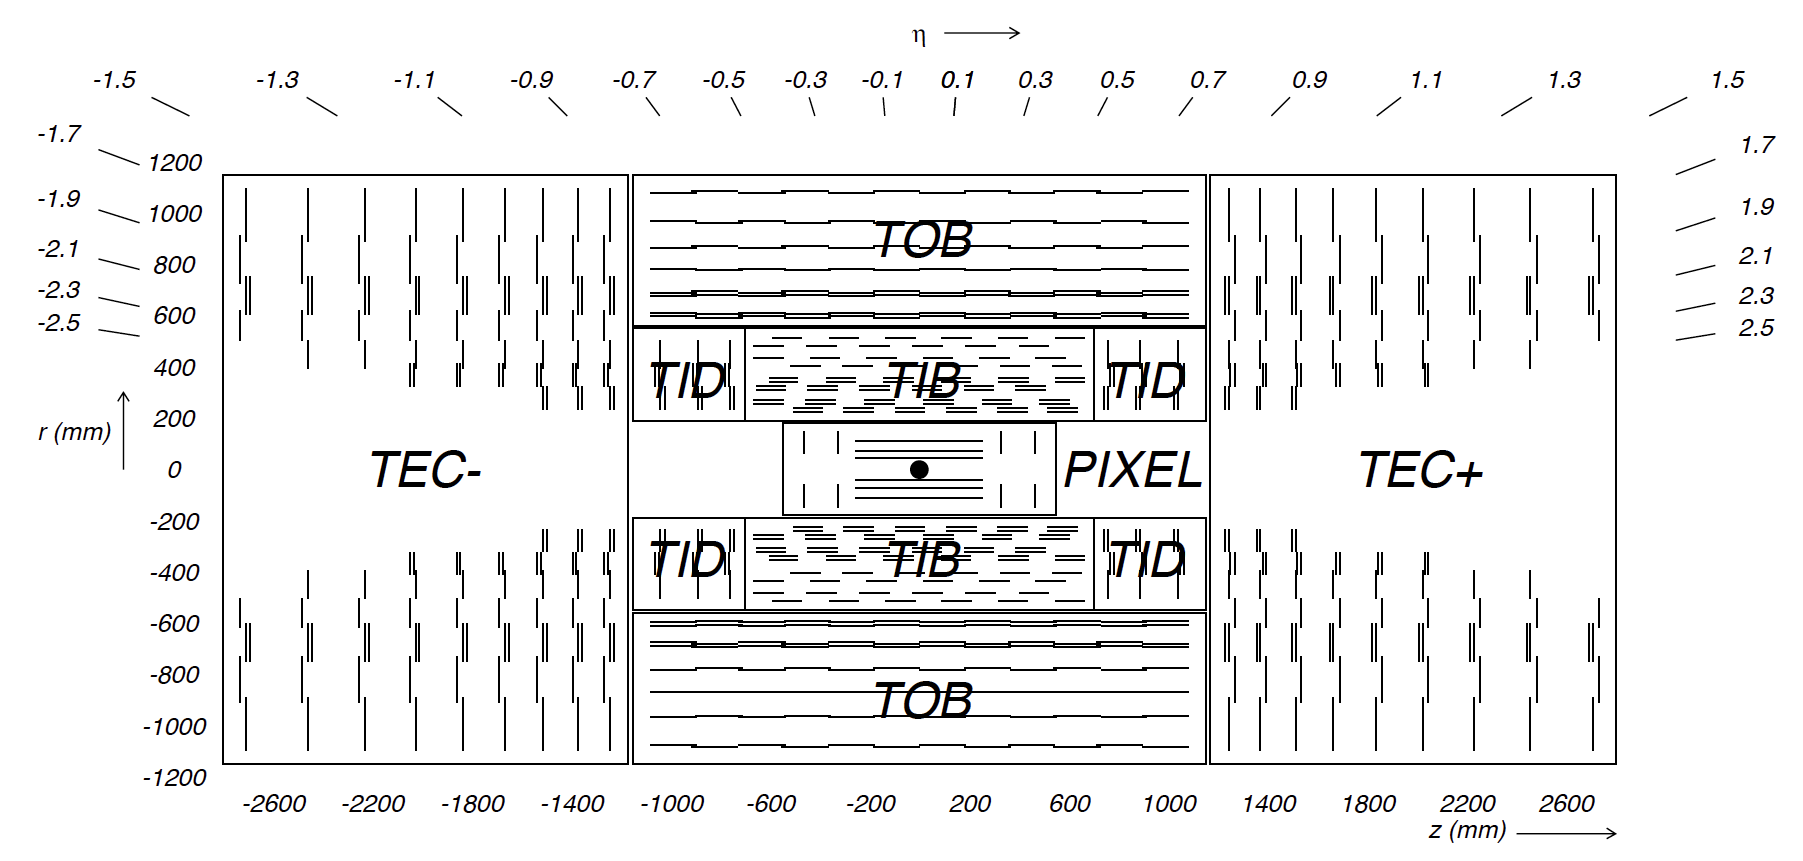
\includegraphics[width=0.8\textwidth]{chapter3/Tracker_structure.png}
\caption{The structure of tracker in CMS~\cite{CMS_experiment}}
\label{fig:tracker_sketch}
\end{figure}



\subsection{The electromagnetic calorimeter}

The CMS Electromagnetic calorimeter(ECAL) is a hermetic homogeneous lead tungstate($PbWO_{4}$) calorimeter. The whole sub-detector is composed of two parts, the central barrel(EB) covering the range $|\eta|<1.479$ and the endcap disks(EE) covering the range $1.479<|\eta|<3.0$. EB is made up of 61200 $PbWO_{4}$ crystals with $22\times22~mm^{2}$ in the front face, 23 cm in length(25.8 in radiation lengths). EE is made up of 7324 crystals per disk with front face $29\times29~mm^{2}$, 22 in length(24.7 in radiation lengths) and a preshower detector(ES)~\cite{CMS_TDR}. The geometrical configuration of ECAL is shown in Figure.~\ref{fig:ECAL_sketch}. 

The $PbWO_{4}$ crystals used in ECAL have high density(8.28 $g/cm^{3}$), short radiation length(0.89 cm) and small Moli$\grave{e}$re radius(2.2 cm), together with the specific geometrical parameters used, rendering ECAL  good energy resolution, fast response, fine granularity and radiation resistant. Photodetectors are placed at the end of the crystals. In EB, avalanche photodiodes(APDs) are used, while vacuum phototriodes(VPTs) are used in EE. Both types of the photodiode show good performance in the environment with hard radiation and 4-T magnetic field. ES is in front of EE in the pseudorapidity range $1.653<|\eta|<2.6$. ES is a sampling detector with silicon strip sensors placed behind the lead radiator to measure the energy and position of the incoming particles.  

\begin{figure}[htbp] 
\centering
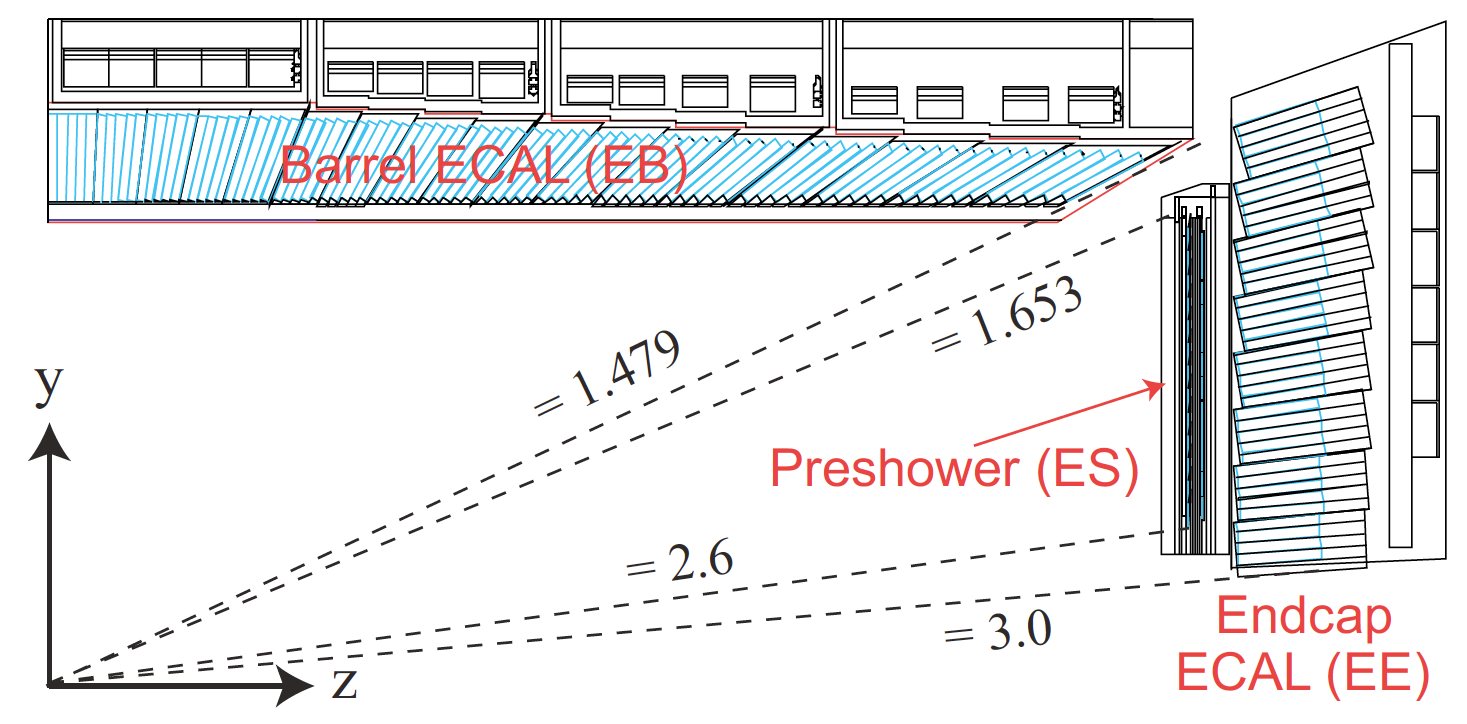
\includegraphics[width=0.8\textwidth]{chapter3/ECAL_transverse.png}
\caption{ECAL geometrical configuration~\cite{CMS_TDR}}
\label{fig:ECAL_sketch}
\end{figure}

Each half of EB is composed of 18 supermodules that one contains 1700 crystals. The $PbWO_{4}$ crystal relative energy resolution is measured with ECAL supermdules directly exposed to electron beam without considering the materials in front as the case in reality. The relative energy resolution as a function of electron energy can be expressed as 
%spikes
% np scattering in the protective epoxy coating of the APD, and the resulting proton directly ionizing the APD active volume.
\begin{align*}
\frac{\sigma}{E}=\frac{2.8\%}{\sqrt{E/\textrm{GeV}}}\oplus\frac{12\%}{E/\textrm{GeV}}\oplus 0.3\%
\end{align*}

The first term stands for the contribution from stochastic factors, like the number fluctuation in production of the secondary particles. The second term is the noise contribution coming from electronics and digitization, while the last is a constant term that covers the other factors~\cite{ECAL_EB_reso}.

\subsection{The hadron calorimeter}

CMS hadron calorimeter(HCAL) is a hermetic sampling calorimeter, which is important for the measurement of the energy and momentum of hadrons, also the missing energy that caused by the non-interacting particles.  HCAL is composed mainly by HCAL barrel(HB), HCAL endcaps(HE) and forward calorimeter(HF). The mechanical structure of HCAL is shown in Figure.~\ref{fig:HCALL_sketch}. 

\begin{figure}[htbp] 
\centering
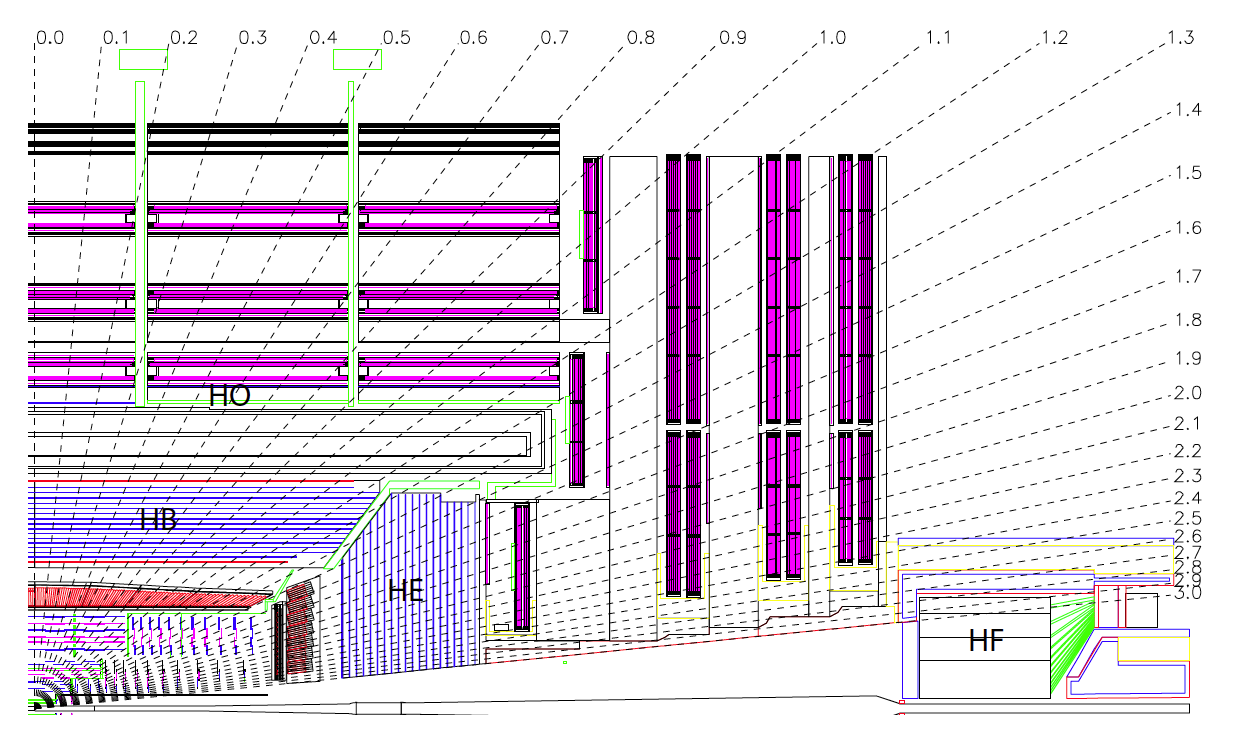
\includegraphics[width=0.8\textwidth]{chapter3/HCAL_sketch.png}
\caption{A longitudinal view of CMS HCAL sub-detector~\cite{CMS_experiment}}
\label{fig:HCALL_sketch}
\end{figure}


HB is mostly composed of  several layer of brass absorber plates, between which are the plastic scintillator tiles. The inner most and out most layer plates are made of stainless steel to gain structural strength. When hadrons hit the absorber, secondary particles are produced in showers. As the showers develops, the alternating layers of scintillators are activated and emit blue-violet light. The lights are collected as signals. HB covers the central pseudorapidity range $|\eta|<1.3$ with a individual read out unit $\Delta \eta\times\Delta\phi=0.087\times 0.087$. To have enough sampling depth in HCAL central region because of the limited spaces between ECAL and muon detector, an extra outer calorimeter(HO) is installed.  HO utilizes the outside solenoid coil as additional absorber to insert plastic scintillators. Similar to HB, HE is also made of brass absorber and plastic scintillator tiles layers, which covers the range $1.3<|\eta|<3.0$. The read out units has the geometry $\Delta \eta\times\Delta\phi=0.17\times 0.17$ in HE~\cite{CMS_experiment}. An combined ECAL and HCAL energy resolution~\cite{HCAL_reso} measured in test beam with pions is 

\begin{align*}
\frac{\sigma}{E}=\frac{110\%}{\sqrt{E/\textrm{GeV}}}\oplus 0.9\%
\end{align*}

HF situates $\pm11$ m from the interaction point to complement the large pseudorapidity measurement of HE in the range $3.0<|\eta|<5.0$. HF is made of grooved steel plates with quartz fibers. Charged shower particles generate Cherenkov light, which is collected by the quartz fibers as signals. Radiation hardness is critical for the operation of HF.   



\subsection{Muon detector}
CMS muon detector is designed to measure the momentum and charge of muons. Three types of gas detectors are used in CMS, the   barrel drift tube(DT) chambers, the cathode strip chambers(CSC) in the endcaps and resistive plate chambers(RPC) in both barrel and endcap regions. 

In muon detector barrel(MB), DT chambers and RPCs are used which covers the pseudorapidity region $|\eta|<1.2$. MB is composed of 250 chambers. The chambers are located in 4 stations inside the magnet return yoke. The yoke is further divided into 5 wheels, each of which is composed of 12 sectors. As shown in Figure.~\ref{fig:muon_sketch}, the stations are named MB1 to MB4, which are composted one DT chamber and varied number of RPCs that depending one the exact location. DT chamber measures the position the incoming muon which knocks off electrons of the gas atoms in the chamber and collected by a large numbers of charged wires inside.% The gas used in DT chambers is a mixture of Ar and $\textrm{CO}_{2}$.

In muon detector endcaps(ME), 468 CSCs which covers the range $0.9<|\eta|<2.4$ are used. ME also composed of 4 stations of chambers and in each of the discs. CSC is in a wedge shape and composed of 6 gas gaps. The gap is filled in with a cathodes strip and anode wires what running perpendicularly to the strip. When a muon comes, the knocked off electrons creating avalanche and received by the positive charged wires.  

Both DT chambers and CSCs measure the position and can also trigger on the $\pt$ of muons. To better deal with the high luminosity and improving the trigger muon $\pt$ resolution, the dedicated trigger system RPCs are added to both MB and ME. RPC is a double-gap bakelite chamber which operates with the avalanches that caused by the muons. RPC can provide additional fast triggering and sharp $\pt$ threshold. Four RPCs layers are used in the MB first two stations(two each) and another two layers(one each) are used in the last two stations.  In the ME, one RPC layers in each of the first three stations.    



\begin{figure}[htbp] 
\centering
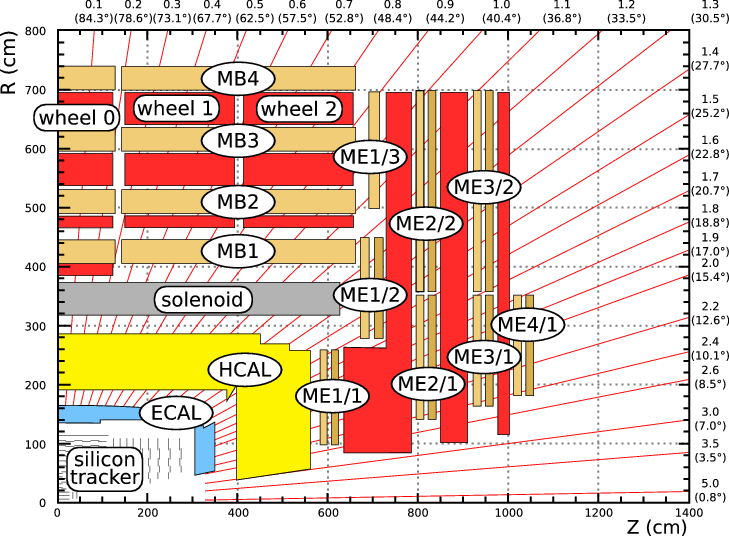
\includegraphics[width=0.8\textwidth]{chapter3/Muon_chambers.png}
\caption{A overview of muon chamber configuration in CMS~\cite{Muon_chambers}}
\label{fig:muon_sketch}
\end{figure}


\subsection{Trigger}

LHC is a high luminosity collider in the order of $10^{34}\textrm{cm}^{2}\textrm{s}^{-1}$. In the p-p collision, the bunch crossing time is 25 ns and the corresponding frequency is 40 MHz. In each of the 25 ns, there are approximately 20 collisions. This high rate makes it impossible to transmit and record all of the events, also it is not necessary, since most of the events are not of current physics research interests. CMS use a two level trigger system to select events and reduce the event recording rate, Level-1(L1) trigger and High-level trigger(HLT) systems. 


L1 trigger is based on custom designed and programmable electronics, situated inside the detector. It utilizes the information from calorimeters and muon system, performing simplified but effective reconstructions, corrections and selections, which reduces the event rate from 40 MHz to 100 kHz. In LHC Run II, the L1 trigger system has been upgraded to deal with the increased luminosity and improve the performance. The L1 calorimeter trigger accesses the information from the whole ECAL and HCAL in the granularity of trigger tower level, which approximately correspond to a region $0.087\times0.087$ in $\eta$ and $\phi$. The trigger reconstructs the $\Pe/\gamma$, jets, $\tau$ and the sum energy of the candidates with the algorithms implemented in the time multiplexed trigger architecture~\cite{TMT_trigger}. The algorithms implemented at hardware trigger level, with dynamic clustering of trigger towers, pile-up migration and innovated tau and jet reconstruction with various look-up table for the calibrations and corrections~\cite{L1_Egamma}. The L1 muon trigger system fully utilizes three muon detectors in the track reconstruction. In general, the track reconstruction of muons are divided into three regions, barrel, overlap and endcap, based on the geometry. Through dedicated construction algorithm, the tracks are built, so as computing the muon qualities. There informations are used in the triggering processes~\cite{L1muontrigger}. 


HLT in CMS further reduced the event rate from 100 kHz(after L1 trigger selection) down to 1 kHz that is a possible rate for event storage. HLT is software based trigger system and utilized the streamlined version of the CMS soft-ware for event reconstruction on the large computer farm~\cite{CMS_trigger_RUNII}. Maximizing the trigger efficiency and keeping acceptable CPU-time is crucial. HLC accesses to the full granularity and sub-detectors of CMS, including the tracker. The dedicated algorithms used in HLT is the very closed to the ones used in the off-line reconstruction and analysis, besides the for some different parameter configurations~\cite{CMS_HLT_RunII}.             








%\subsubsection{Level 1 Trigger}
%probably I have to put something there2



%\subsubsection{High Level Trigger}


%
% Chapter 4 
%


\chapter{Datasets}
\section{Datasets used in LFV analysis}
\subsection{\Hmuhad}
The data sample used in the analysis is from LHC 2016 Runs, recorded by CMS detecter. Total integrated luminosity of the analyzed data is $35.9 ~\textrm{fb}^{-1} $ with center-of-mass energy of $ \sqrt{s}=13 ~\textrm{TeV} $. The data sample labeled in the CMS experiment as SingleMuon\_Run2016B,C,D,E,F,G,H. The name SingleMuon in the data sample represents the trigger used in the analysis, which selects the events with at least a muon passed the trigger selection. Gluon gluon fusion Higgs(ggH)~\cite{Georgi:1977gs} production and vector boson fusion Higgs(VBF)~\cite{Cahn:1986zv} are the main Higgs production channels considered in the analysis. For the background samples, besides the misidentified background which is talked about in detail in Chapter6, the other background samples are all generated with Monte Carlo(MC) simulation.  POWHEG~\cite{POWHEG-BOX} or MadGraph~\cite{Alwall:2014} generator is used for the generation and all of the MC samples, including the signal samples, the parton showering, fragmentation, and decays are performed by Pythia8~\cite{Sjostrand:2014zea}.  Pileup effect is taking into account in the generator by generate minimum bias events simultaneously and a correction is applied by comparing the data sample. The average number of pileup interaction per bunch crossing is 27. CMS detector environment is simulated by GEANT4~\cite{GEANT4}. The details of the MC samples used in the analysis are summarized in Table.~\ref{tab:mutaumcsamples} and Table.~\ref{tab:mutaumcsamples2}.

\begin{table}[!hbpt]
\caption{Monte Carlo samples used in the search, together with their respective cross sections.}
\begin{center}
% sample name   &    generator    & cross section 
\begin{tabular}{|c|c|c|}
\hline
Processes & Generator & Cross section [pb] \\\hline
DYJets$\to\ell \ell$, $m_{\ell \ell}>50$ GeV &MadGraph+pythia8   & 4954.0 \\\hline
DY1Jets$\to\ell \ell$, $m_{\ell \ell}>50$ GeV &MadGraph+pythia8 & 1012.5 \\\hline
DY2Jets$\to\ell \ell$, $m_{\ell \ell}>50$ GeV&MadGraph+pythia8  & 332.8 \\\hline
DY3Jets$\to\ell \ell$, $m_{\ell \ell}>50$ GeV&MadGraph+pythia8  & 101.8 \\\hline
DY4Jets$\to\ell \ell$, $m_{\ell \ell}>50$ GeV&MadGraph+pythia8  & 54.8 \\\hline
DYJets$\to\ell \ell$, $m_{\ell \ell}<50$ GeV&MadGraph+pythia8    & 1861.0 \\\hline
$t\bar{t}$                                                     & powheg+PYTHIA     &  831.76\\\hline
$t \backslash \bar{t}\to t w$                        & powheg+PYTHIA8     &  35.85 \\\hline
$WZ \to \ell 3v$                                          & MadGraph+PYTHIA8   &  3.05   \\\hline
$WZ \to \ell v 2q $                                      & MadGraph+PYTHIA8   &  10.71  \\\hline
$WZ \to 2 \ell 2q $                                      &  MadGraph+PYTHIA8  &  5.595 \\\hline
$t\to4f $                                                     & POWHEG+PYTHIA8       & 136.02\\\hline
$\bar{t}\to4f $                                             & POWHEG+PYTHIA8       & 80.95\\\hline
$WW \to \ell v 2q$                                      & MadGraph+PYTHIA8   &  1.212   \\\hline
$ZZ \to 2\ell 2q $                                        & MadGraph+PYTHIA8    &  3.22   \\\hline
$VV \to2\ell 2 q$                                        &  MadGraph+PYTHIA8   &  11.95  \\\hline

\end{tabular}
\end{center}
\label{tab:mutaumcsamples}
\end{table}

\begin{table}[!hbpt]
\caption{Continue with MC samples used in the analysis.}
\begin{center}
\begin{tabular}{|c|c|c|}
\hline
MC simulations & Generator & Cross section [pb] \\\hline
$VV \to2\ell 2 q$                                        &  MadGraph+PYTHIA8   &  11.95  \\\hline
$ggH\to \Pgt\Pgt $                                      & POWHEG+PYTHIA8 &      3.046\\\hline
$\textrm{VBF}H\to \Pgt\Pgt $                     & POWHEG+PYTHIA8 &      0.237\\\hline
$ggH\to WW \to 2\ell 2v$                            & POWHEG+PYTHIA8 &      1.103\\\hline
$\textrm{VBF}H\to WW\to 2\Pl 2v$             & POWHEG+PYTHIA8 &    0.086\\\hline
$ZH \to \Pgt\Pgt$                                        & POWHEG+PYTHIA8 &    0.055\\\hline  
$W^{-}\backslash W^{+} H\to\Pgt\Pgt$        & POWHEG+PYTHIA8 &    0.086\\\hline 
$ttHJet \to \Pgt\Pgt$                                   &MadGraph+PYTHIA8&     0.32\\\hline   
\end{tabular}
\end{center}
\label{tab:mutaumcsamples2}
\end{table}


\subsection{\Hehad}

The search of lepton flavour violation Higgs decay $\Hehad$  is performed with CMS 2012 RunI dataset at center-of-mass energy  $\sqrt{s}=8 ~\textrm{TeV}$. The dataset is named as SingleElectron\_Run2012A,B,C,D with an integrated luminosity of $19.7 ~\textrm{fb}^{-1}$. Single electron HLT tigger is used which is talked more in details in Chapter 5. A detail list of simulation samples used in the analysis is listed in Table.~\ref{tab:mcdatasets}.  For the signal samples, ggH and VBF Higgs production channels are the main channels considered. For background samples, besides $Z\to \tau \tau$ which is produced with embedding technique and misidentified background which is estimated with data-driven method are produced with MC simulation. Various simulation packages are used. Signal samples are produced with PYTHIA8, which uses sophisticated $\tau$-lepton decay machinery. Tauola~\cite{Simulation:Tauola} is also used for the simulation of $\tau$ lepton decay in some of samples. CMS detector environment is simulated by GEANT4. 


\begin{table}[hbtp]
 \begin{center}
  \caption{Signal and background MC samples}
  \label{tab:mcdatasets}
  \begin{tabular}{l|l|l}
Processes & Generator & Cross section [pb] \\\hline
$ggH\to e\tau $     &          PYTHIA8                     &  19.27                \\\hline
$VBH\to e\tau$     &          PYTHIA8                      &   1.58                \\  \hline
$ggH \to \tau\tau$ &POWHEG+PYTHIA6              &  19.27           \\\hline
 $VBF\to\tau\tau$  &POWHEG+PYTHIA6              &   1.58           \\  \hline
$t\overline{t}+\textrm{jets}~ \textrm{full}~\textrm{leptonic}$  &  MadGraph+Tauola                &  26.20                \\\hline
$t\overline{t}+\textrm{jets}~\textrm{Semi}~\textrm{leptonic}$   & MadGraph+Tauola           &  109.28               \\ \hline
$t \to tw$              &   POWHEG+Tauola     &    56.4 \\\hline
$\bar{t} \to tw$              &   POWHEG+Tauola     &    30.7 \\\hline
$t$,$\bar{t}(\textrm{T channel})$           & POWHEG+Tauola        &   11.1 (11.1)          \\ \hline
$WW \to 2l2\nu+jets$    & PYTHIA6+Tauola                  & 5.824\\ \hline
$ZZ\to 4l$               & MadGraph+Tauola                 & 0.18                  \\  \hline
$ZZ\to 2l2Q$             &MadGraph+Tauola              &   2.502               \\  \hline
$ZZ\to 2l2\nu$           &MadGraph+Tauola              &    0.716              \\  \hline
$WZ\to 2l2Q$             &MadGraph+Tauola                &    2.21               \\  \hline
$WZ\to 3l\nu$            &MadGraph+Tauola           & 1.06                  \\  \hline
  \end{tabular}
 \end{center}
\end{table}





\section{Event reconstruction}
In this section, a general presentation of the event reconstruction algorithm used in CMS, particle-flow(PF) reconstruction is shown. A more detail information about the reconstruction of tracks and the objects related to the lepton flavour violation higgs decay are in the following section. 
\subsection{Particle flow algorithm}

Particle flow event reconstruction algorithm is the main algorithm used in CMS. PF performs a global event reconstruction~\cite{CMS-PRF-14-001}, which aim to utilize the information from the whole detector to identify individual particles in each event.



\subsubsection{Tracking and Calorimeter algorithm}\label{PFtracker}

In the PF algorithm, the reconstruction of charged particles in the inner tracker is a crucial part. In this section, the reconstruction of the trajectories of charged particles, especially the electron and muon reconstruction is discussed. 

Inner tracker is aimed at measuring the track of energetic charged particle. The track finder is based on the Kalman Filtering(KF)~\cite{tracker:algo}. This reconstruction comes in a couple steps. First an initial seed is generated from a couple hits that compatible with a track in the tracker, then a trajectory is builded with the seed and other hits from the tracker along this track. At last a fit is perform on the track  to determine the properties of this particle candidate, like the momentum, the charge and the direction. The qualities that can affect the performance of the reconstruction are like the number of hits in the pixel detector, the total number of hits in the tracker, the distance from the cylinder and the energy of this charged particle. This is discussed in more details later.

The performance of the track reconstruction is measured in reconstruction efficiency and misreconstruction rate. The reconstruction efficiency is defined as the ratio of track reconstructed with more than 50\% hits from simulated hits and the total simulated tracks. The misreconstruction rate is defined as the fraction of the tracks can not be associated with simulated tracks of the whole simulated tracks.  If a charged hadron is not identified by the tracking algorithm, then the hadron is take as a neutral hadron and measured by the calorimeters. This will affect the jet energy and position resolution. Improving the track reconstruction efficiency while keeping the misreconstructed rate low is critical for PF reconstruction.

In CMS, an iterative tracking is perform, in which the reconstruction of tracks is done is a couple steps. Each step is aimed for a moderate efficiency but with a high purity. After one step, the hits that used to form tracks are masked and a next step is perform. This iterative tracking is down in ten steps if necessary and the detail information is shown in Table.~\ref{tbl:iterative_tracking} and more can be found in \cite{CMS-PRF-14-001}. In the table, the name column points out the processes that that step of iteration is aiming at. The seeding column shows the requirement on the seeding, while the targeted tracks column shows the characters of the tracks.

Electron is one of the main particle understudy in $\Hehad$ search. In CMS, electron track reconstruction is taken as a merge of ECAL based and tracker based strategy. The tracker based seeding strategy is as described above, besides the case when energetic photons are radiated, then a preselection based on the number of hits and $\chi^{2}$ of the fit is set with the Gaussian-sum filter~\cite{Algo:GSF}. The ECAL based electron seeding strategy building the superclusters(SC) to gathering the bremsstrahlung photons. The energy of the SC is taken as the energy sum of the cell crystals inside and the position is evaluated with energy weight. The electron trajectory in the first layer of the the tracker is estimated and the seed from the track is selected. This works in the case when there is not much bremsstrahlung photons, then most of the energy is deposited in ECAL. In the case when soft photons are radiated mostly, ECAL based seeding may still performs well. But when the electrons are in the jets or low energy, either electron contributions are overlapping with other particle or the radiation and bending is too much, it is hard to recover these electrons with ECAL based algorithm only. The ECAL based and tracker based electron seeding is merged into one collection, which significantly improves the reconstruction efficiency.



\begin{table}[!tpb]
\caption{Iterative tracking steps take in CMS \label{tbl:iterative_tracking}}
\label{tab:antil}
\begin{center}
\begin{tabular}{|llll|}   
\hline
Iteration                   &  Name               &   Seeding            &  Targeted Tracks  \\\hline
1                              & InitialStep          & pixel triplets        &  prompt, high $p_{t}$   \\
2                              & DetachedTriplet          & pixel triplets        &  from b hadron decays, R$\lesssim$ 5 cm  \\
3                              & LowPtTriplet          & pixel triplets        &  prompt, low $p_{t}$ \\
4                              & PixelPair          & pixel pairs                &  recover high $p_{t}$ \\
5                              & MixedTriplet          & pixel+strip triplets                &  displaced,  R$\lesssim$ 7 cm   \\
6                              & PixelLess          & strip triplets / pairs               &  very displaced, R$\lesssim$ 25 cm     \\
7                              & TobTec          & strip triplets / pairs               &  very displaced, R$\lesssim$ 60 cm     \\
8                              & JetCoreRegional          & pixel+strip pairs               &  inside high $p_{t}$ jets    \\
9                              & MuonSeededInOut          & muon-tagged tracks               &  muons   \\
10                            & MuonSeededOutIn          & muon detectors                &  muons   \\\hline
\end{tabular}
\end{center}
\end{table}


Calorimeters are crucial components for the PF algorithm in CMS. The clustering algorithm in calorimeters is used to identify neutral stable particles like phone and neutral hadron, together with tracker in the identification of charged particles, reconstructing the energy of electrons and the possible associated bremsstrahlung photons and measuring the energy of charge particles that are missed by the tracker.  

The clustering algorithm is perform separately in each sub-detector system beside the HF in which each cell directly raise a cluster. The algorithm starts by finding a cluster seed. Then a topological walking around the neighbouring cells is performed. Both seed cells and neighbouring cells are required to pass certain thresholds to construct high quality candidates and suppress the contribution from noise. In ECAL endcaps, additional requirements on $E_{T}$ because of the high noise level. In each of the topological clusters, the energy for the neighbouring cells are assumed from the seed cells. A Gaussian-mixture model is used in the construction of the topological clusters to evaluate the contribution of each cells. The finally parameters of the model is obtained by analytical fitting to the Gaussian model which give the maximum expectation.

To accurately measure the energy of particles like photons and neutral hadrons, the calibration of calorimeters is indispensable. The calibration of calorimeter also affects identification efficiency and misidentification rate of the particles measured in the calorimeters. The calibration of ECAL is done with a couple source, like the test beam, the radioactive source and the cosmic ray measurements and refined with the collision data. There are thresholds used in the formation of topological clusters, which results in the energy measured is smaller than the incoming particle energy. A residual energy calibration is applied to all ECAL clusters to account for these affects with simulation samples.  The correction is applied as a function cluster energy and position, $f(E,\eta)=g(E)h(\eta)$. In the endcaps, the energy is taken as a liner combination of ECAL and preshower energy, the parameters in the combination is optimized by the $\chi^{2}$ method. Hadrons generally leave energy in both ECAL and HCAL. The calibration of ECAL mentioned above is for the photon, electron calibration. The behavior of hadron is different and a consequent calibration involving both ECAL and HCAL is needed. Simulated single neutral hadrons is used. The relationship involving both the energy measured by ECAL and HCAL and the calibrated energy $E_{calib}$ is expressed as

\begin{align*}
E_{calib}=a+b(E)f(\eta)E_{\textrm{ECAL}}+c(E)g(\eta)E_{\textrm{HCAL}}
\end{align*}

In the equation, a is independent of E and accounts for the effects of thresholds in the clustering algorithm. The other coefficients are determined by the $\chi^{2}$ optimization with the $E_{calib}$ and true energy E from simulation. 



A detail description of particle flow algorithm can be found in~\cite{CMS_PRF_14_001}.

\begin{figure}[htbp] 
\centering
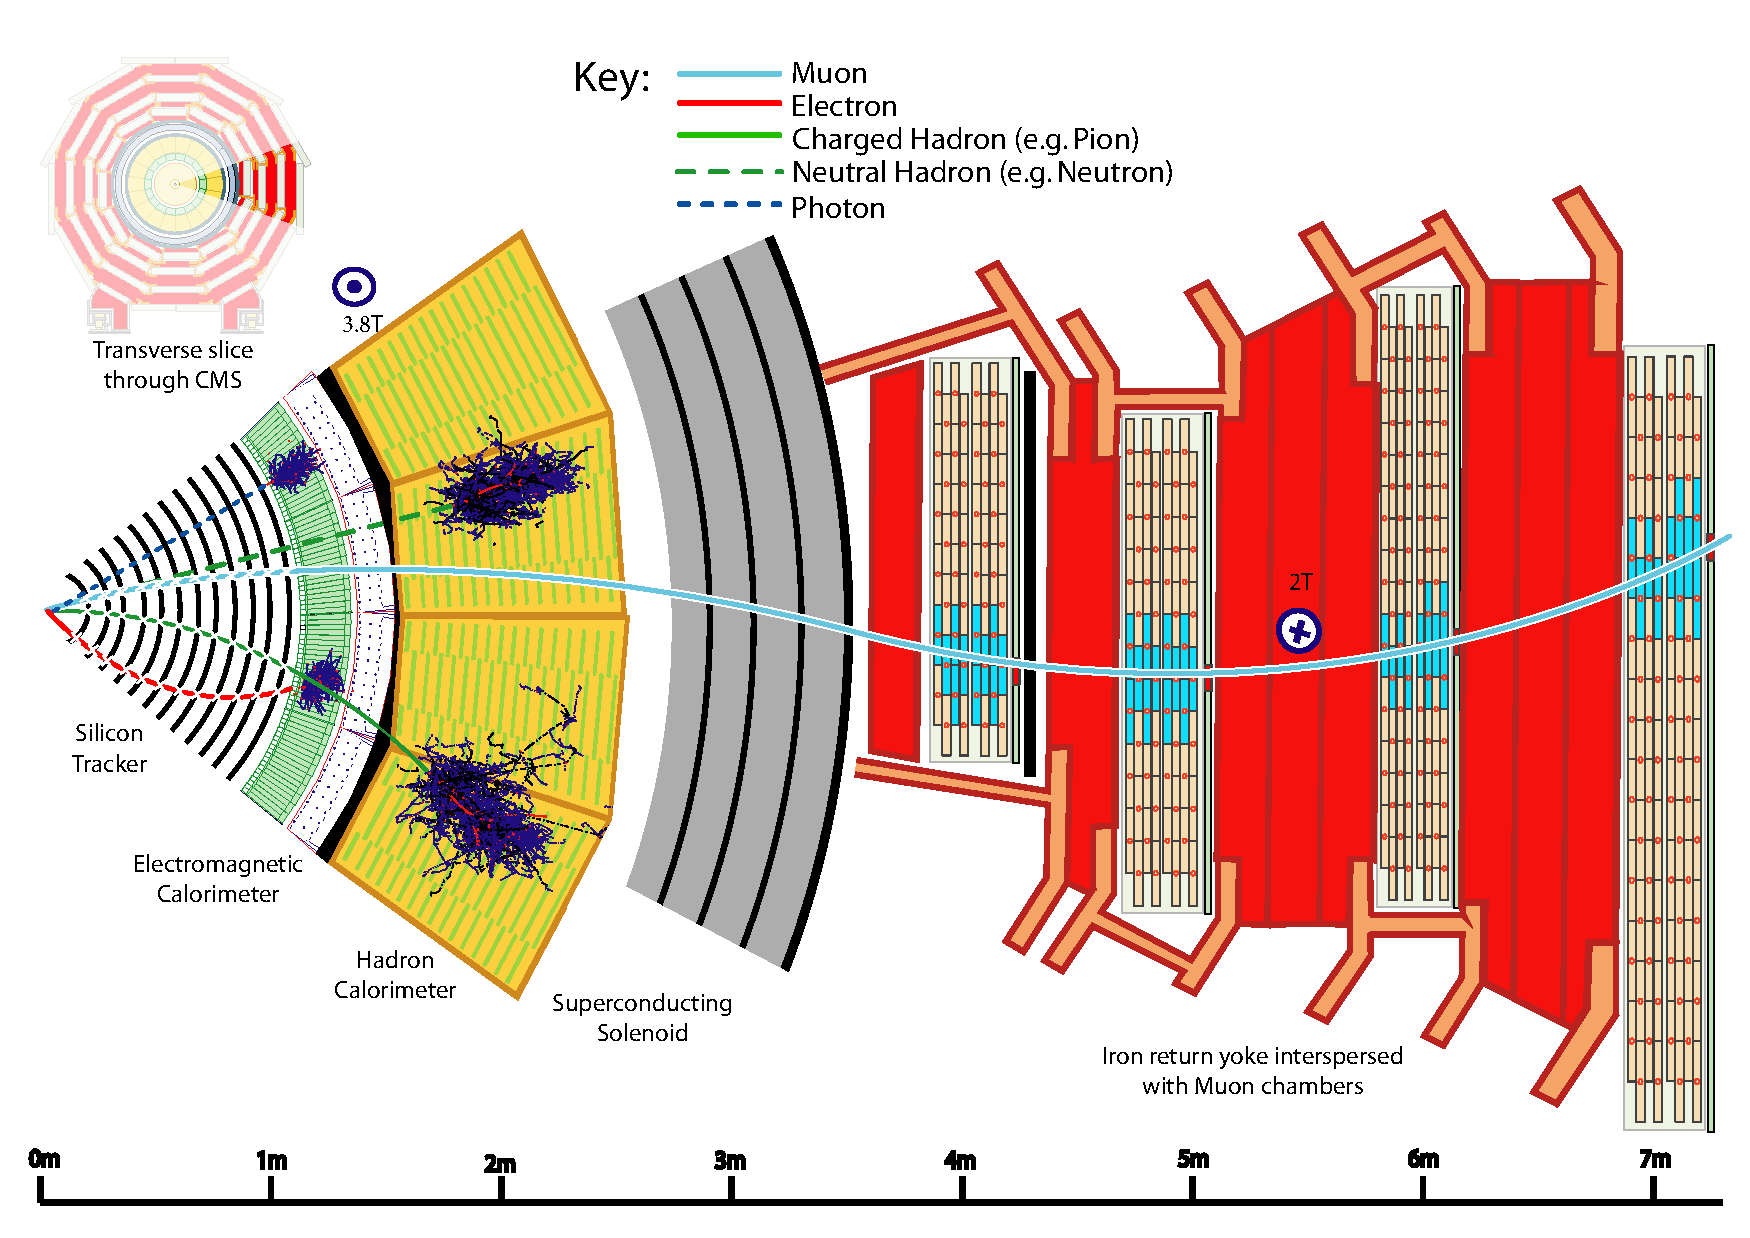
\includegraphics[width=0.6\textwidth]{chapter4/CMS_detecter_slice.pdf}
\caption{A sketch view of CMS detecter. Examples are given to show how the particles interact with different sub-detecters.}
\label{fig:CMSslice}
\end{figure}



\subsection{Muon reconstruction and selection criteria}

PF muon is used in the $\Hmuhad$ analysis. In CMS, the event reconstruction starts from building the tracks in tracker(tracker track) and muon system(standalone-muon track) separately. Global muon reconstruction and tracker muon reconstruction are based on these tracks. ~\cite{muonreco}. Global muon reconstruction starts from the standalone-muon tracks and requires at least two muon station in the muon system. For each of the standalone-muon track, a propagating is done to find a matching tracker track on the common surface. Kalman-filter technique~\cite{Fruhwirth:1987fm} is used in the fitting to combine the hits in standalone-muon track and tracker track. The tracker muon starts from the tracks with $\pt>0.5$GeV and total momentum $p>2.5$ GeV. The tracks are then extrapolated to match the tracks in the muon system with at least one muon segment.  Within the geometry acceptance of muon system, the muon reconstruction efficiency is high, especially high momentum muons, constructed as either global muon or tracker muon or both has the  efficiency about 99\%.  PF reconstruction utilizes the whole detector information to identify and reconstruct all of the particle. The muon PF algorithm applies a series of selections to the global muon and tracker muon to select out the PF muon. The selection is optimized to identify the muons in the jets with high efficiency and low misidentify rate. The details of the selection is in~\cite{PFmuonselection}.   



With the PF muon as the input, muons used in the analysis are further categorized into different identification, isolation categories. Muon ID suggested in CMS RunII, for the LHC data 2016, running period BCDEF, ICHEP medium muon ID is applied(table~\ref{tbl:ICHEPMedID}), for running period G and H, also the monte Carlo samples, standard medium muon ID(table~\ref{tbl:standardMedID})are applied to achieve the best performance for muon identification. 

%In the compatibility-based selection, two ?compatibility? variables are constructed, one based on calorimeter information and the other based on information from the
%muon system. A tracker muon is considered to be a muon candidate if the value of a linear combination of these variables is larger than a pre-defined threshold.
%The segment compatibility, which can have values between 0 and 1, describes the quality of the spatial
%agreement between muon segments and the reconstructed track of the muon candidate


%The kink finder algorithm searches for an interaction of the studied particle with the layers of the
%tracking system by performing a fit of the section of the track before the layer with the one after the
%layer. If an interaction happened, the fit will not work properly because of a change in curvature of
%the track.



\begin{table}[!tpb]
\caption{Muon ID used in the analysis, for the LHC data 2016, running period BCDEF.  \label{tbl:ICHEPMedID}}
\label{tab:antil}
\begin{center}
\begin{tabular}{|l|c|}   
\hline
ICHEP mediumID description                    &  Technical description\\\hline
Loose muon ID                               & PFLoose Muon\\\hline
Fraction of valid tracker hits           & $>0.49$ \\\hline
\multirow{5}{*}{1.Good Global muon}                      &Global muon\\\cline{2-2}
                                                                        &Normalized global-track $\chi^{2}<3$\\\cline{2-2}
                                                                        &Tracker-Standalone position match $< 12$\\\cline{2-2}
                                                                        &kick finder $< 20$ \\\cline{2-2}
                                                                        &Segment compatibility $> 0.303$ \\\hline                                                                       
\hline
2. Tight segment compatibility      & Segment compatibility $>0.451$\\\hline
\end{tabular}
\end{center}
\end{table}


\begin{table}[!tpb]
\caption{Muon ID used in the analysis, for the LHC data 2016, running period G and H, also the monte Carlo samples.  \label{tbl:standardMedID}}
\label{tab:antil}
\begin{center}
\begin{tabular}{|l|c|}   
\hline
Standard mediumID description                    &  Technical description\\\hline
Loose muon ID                               & PFLoose Muon\\\hline
Fraction of valid tracker hits           & $>0.8$ \\\hline
\multirow{5}{*}{1.Good Global muon}                      &Global muon\\\cline{2-2}
                                                                        &Normalized global-track $\chi^{2}<3$\\\cline{2-2}
                                                                        &Tracker-Standalone position match $< 12$\\\cline{2-2}
                                                                        &kick finder $< 20$ \\\cline{2-2}
                                                                        &Segment compatibility $> 0.303$ \\\hline                                                                       
\hline
2. Tight segment compatibility      & Segment compatibility $>0.451$\\\hline
\end{tabular}
\end{center}
\end{table}


\subsection{Electron identification}

Electrons in CMS is constructed with the information from tracker and calorimeters. One of the main difficulties is the bremsstrahlung emitted by the electron during the traveling among the detector materials. The conversion of the photons from the bremsstrahlung affect the reconstruction of tracks in the track and these phones also cause significance energy loose in the electron reconstruction. The construction of Electron is discussed in section~\ref{PFtracker} and more details can be found in~\cite{electron_reco2015}. 

Electron ID is constructed to separate Prompt isolated electron(signal) from the background processes. The background can be the electrons from photon conversion, from quark semi-leptonic decay and from misidentification of other particles or jets. The variables used in the identification are related to tracker and ECAL.  There are mainly three types of variables. The variable related only to calorimeters. For example, the cluster shape of real electron in ECAL is usually narrower than the shape from hardonic showers and electrons leave most of the energy in ECAL and the energy ratio between ECAL and HCAL is large. The variables related to the matching of measured energy and geometry between tracker and ECAL. The variables related to tracker fitting to explore the difference between electrons and hadrons. These related variables can be used to construct cut-based selection sequence to selection electron. To achieve better performance, MVA based ID with boosted decision tree is also trained. Compared with the cut-based selection, more variables in the three categories mentioned above are used in the training~\cite{electron_reco2015}.  An example of the BDT electron ID is shown in Figure.~\ref{fig:eleBDTID}


\begin{figure}[!htbp] 
     \centering
     \subfigure[EB]{ 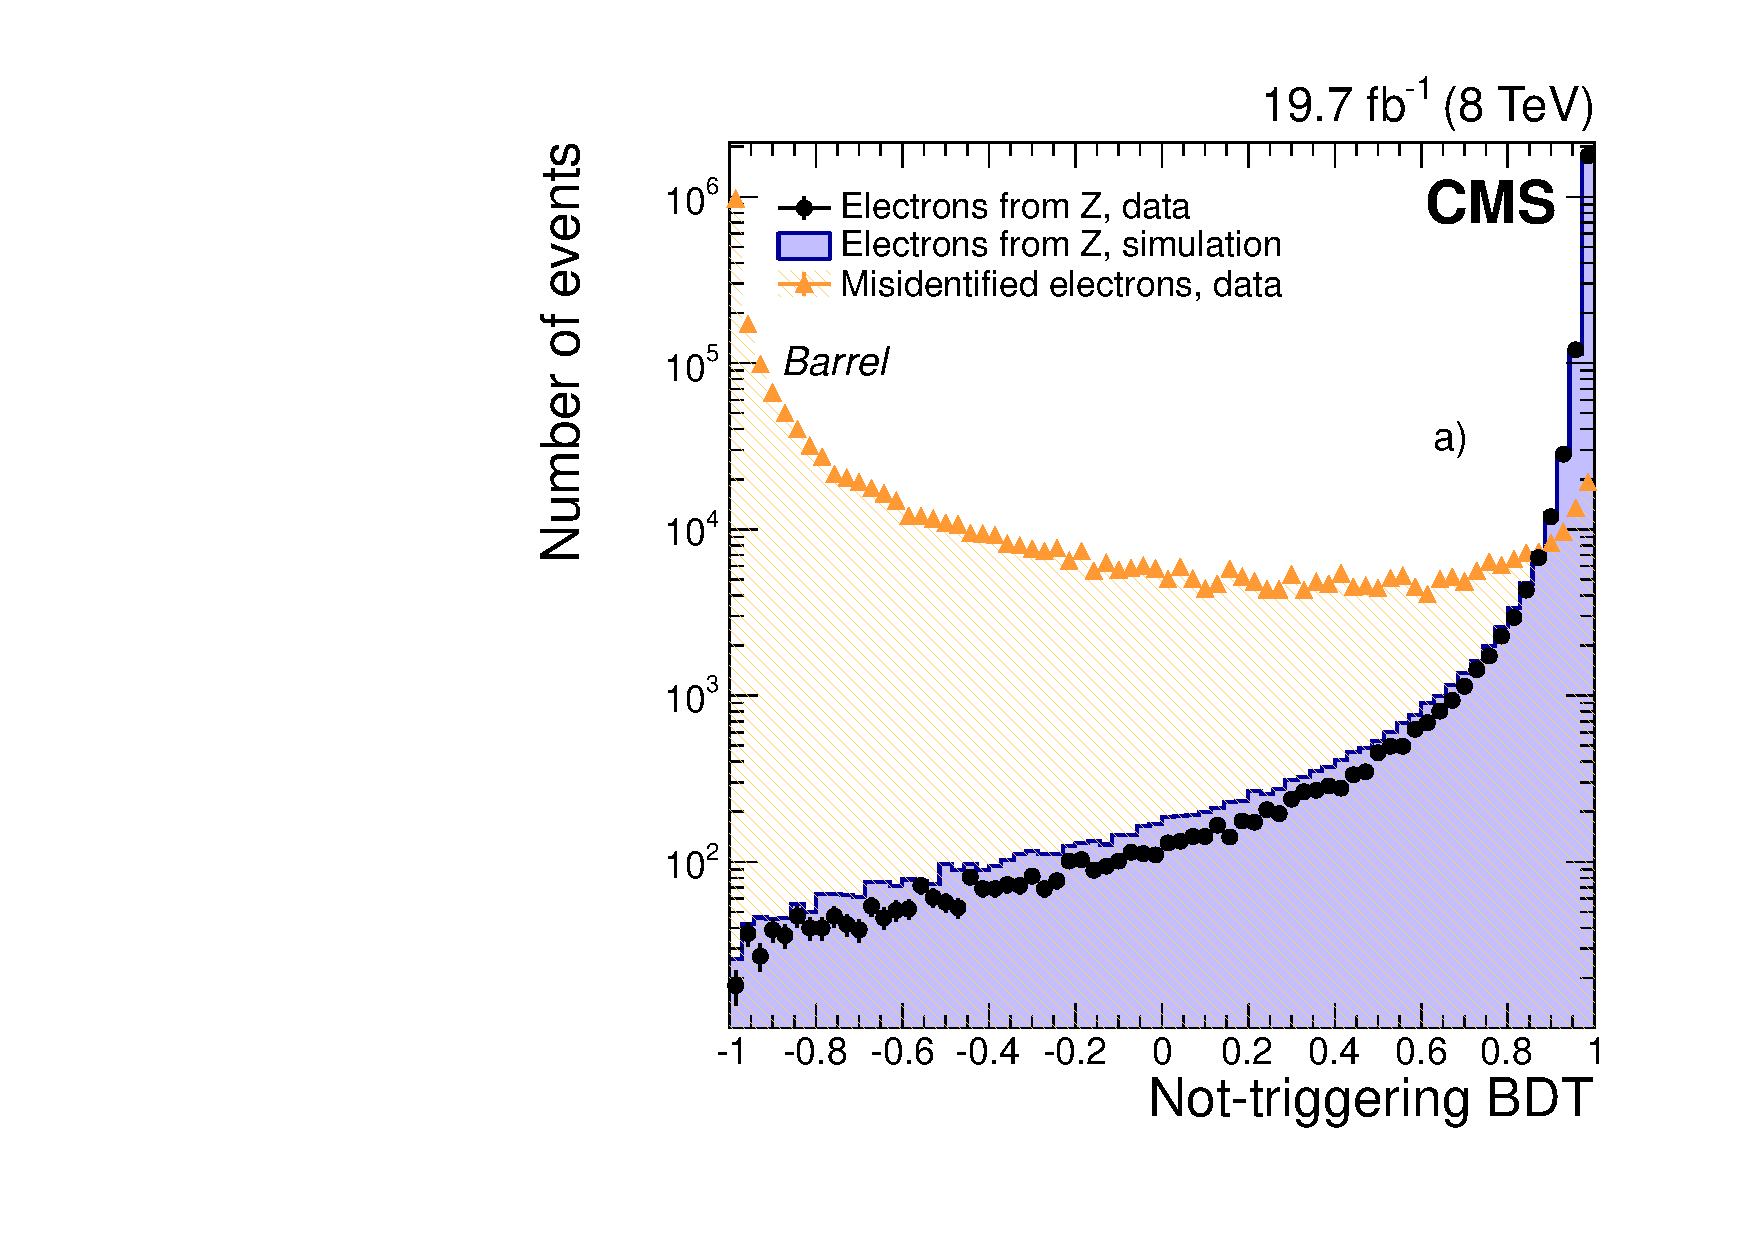
\includegraphics[width=0.4\textwidth]{chapter4/EleID_EB_BDT_perfor.pdf}}
     \subfigure[EE]{ 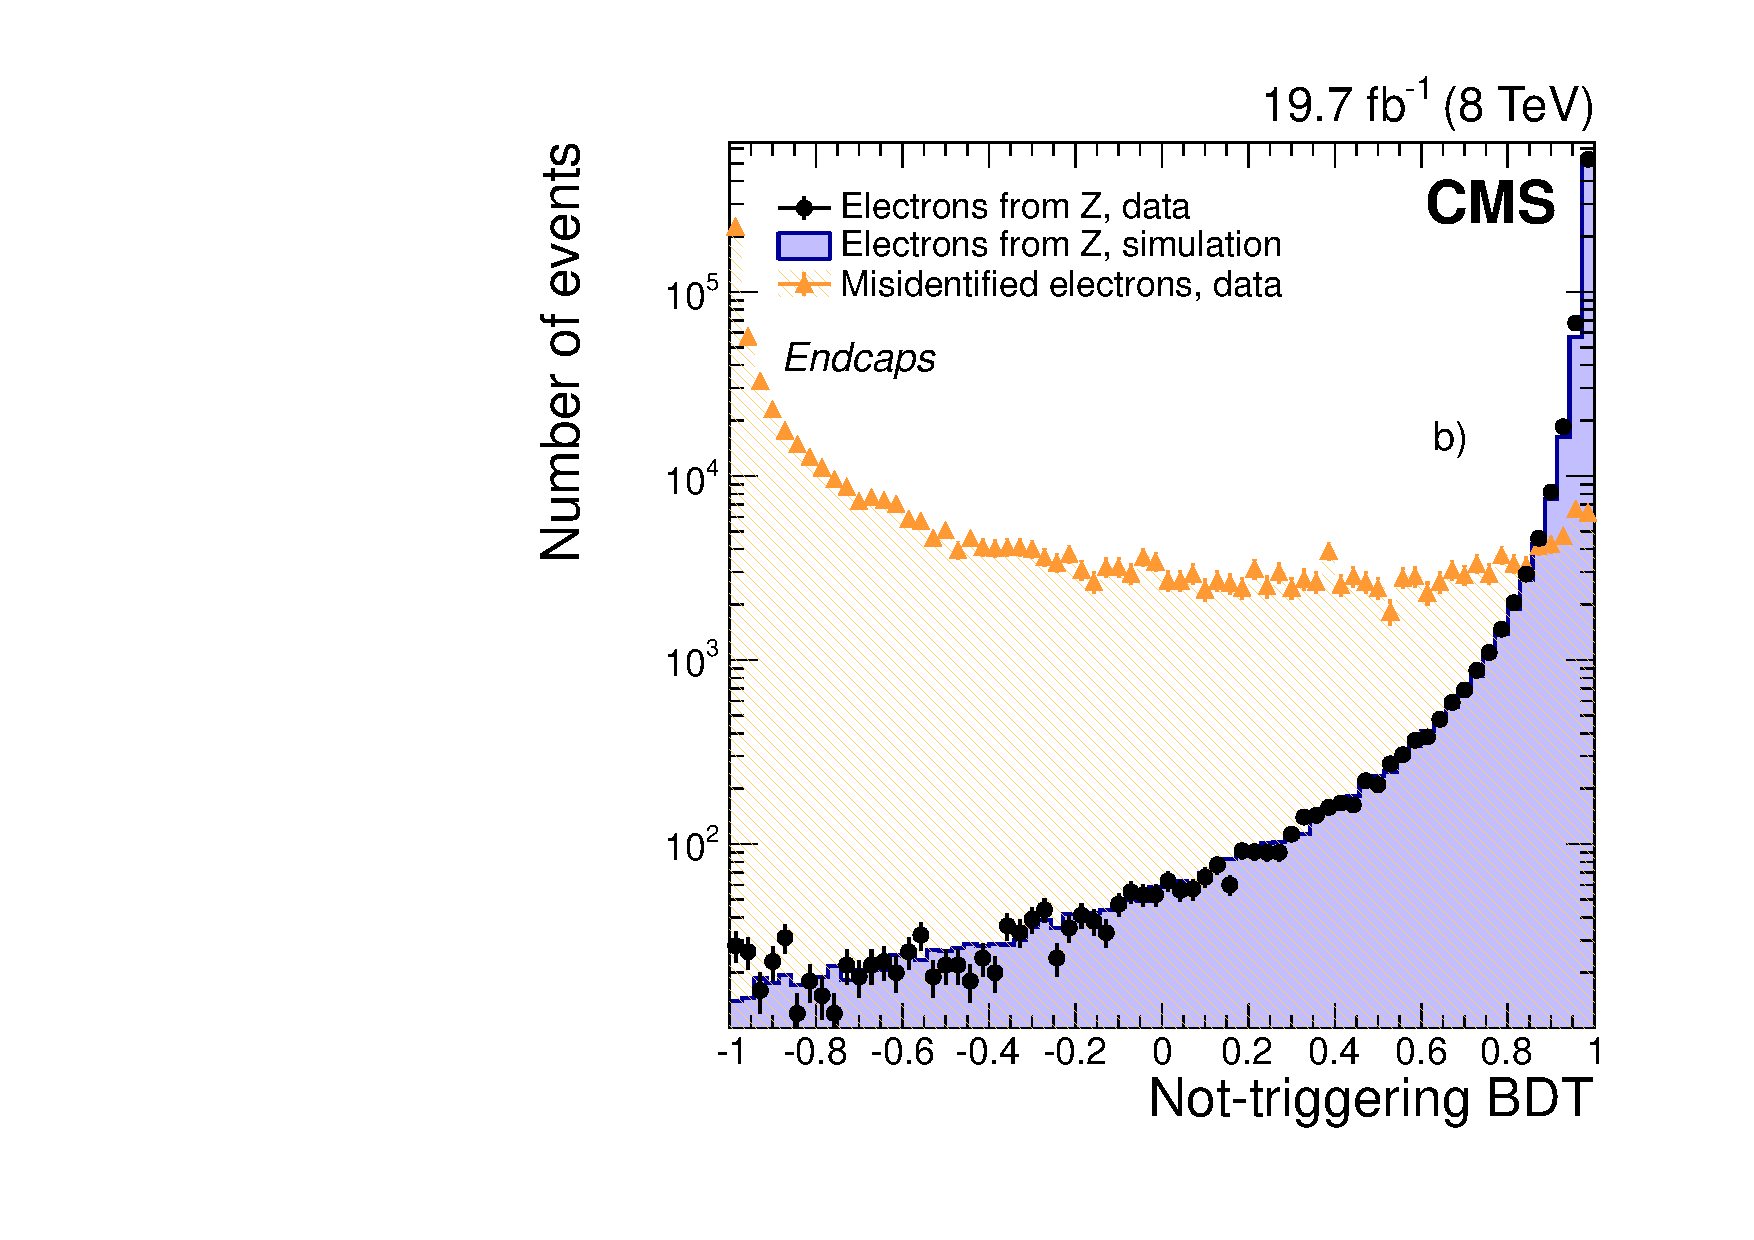
\includegraphics[width=0.4\textwidth]{chapter4/EleID_EE_BDT_perfor.pdf}}\\
     \caption{Electron BDT-based ID shows good discriminating power against background in both EB and EE~\cite{electron_reco2015}}
     \label{fig:eleBDTID}
\end{figure}


Electron isolation is used to reject background events in addition to the ID variables, also inverting the requirement in the isolation can be used to setup enriched background control regions. Large numbers of background events that can possible enter the signal selection are misidentified jets or the jets in which there are real electrons, for example the jets from b quark semi-leptonic decay. For these background events, one key different character with respect to signals is more energy flowing around the electron(or misidentified electron) trajectory. The isolation requirement used in HLT level is summing over the energy depositions either in ECAL or HCAL in the certain core, for example $\Delta R=0.3,0.4$, $\Delta R=\sqrt{\Delta \phi^{2}+\Delta\eta^{2}}$. The contribution from the particle candidate is removed. In the offline algorithm, particles can better identified with the PF algorithm. Similar in concept to the isolation using the energy flow, the PF isolation summing over the $\pt$ of the particles in the direction of the reconstructed candidate trajectory momentum. PF algorithm utilizes the whole detector information and the isolation is defined as

\begin{align*}
\textrm{Iso}_{\textrm{PF}}=\sum \pt^{\textrm{charged}}+\textrm{max}\bigg[ 0,\sum \pt^{\textrm{neutral~had}} +\sum \pt^{\gamma}-\pt^{\textrm{PU}}\bigg]
\end{align*}

The isolation variable sums over the contribution from charged PF candidates, neutral particles and photons in a certain selected $\Delta R$ region around the signal. The contribution from pileup is estimated with $\pt^{\textrm{PU}}$ with the FASTJET technique~\cite{FastJetalso}. The energy of PF objects are better calibrated and the double counting problem which shows up the energy flow isolation described above is solved. PF isolation variable performs better than the isolation variable used in HLT. The performance comparison is shown in Figure.~\ref{fig:eleIso}

\begin{figure}[!htbp] 
     \centering
     \subfigure[EB]{ 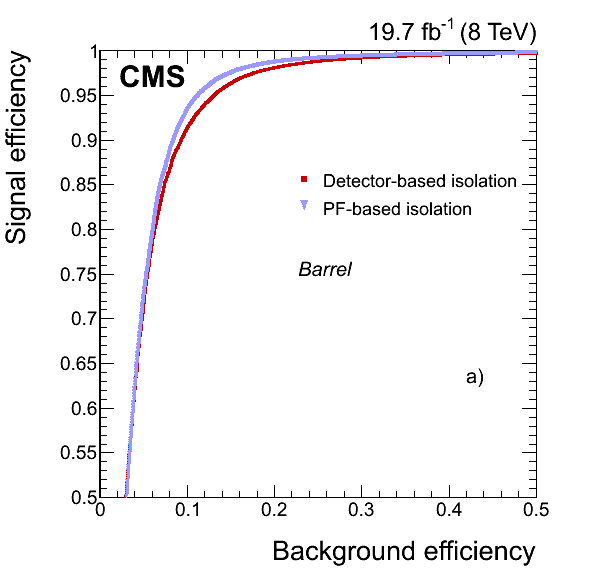
\includegraphics[width=0.4\textwidth]{chapter4/ROC_IsoOnly_Data_EB_HighPt.png}}
     \subfigure[EE]{ 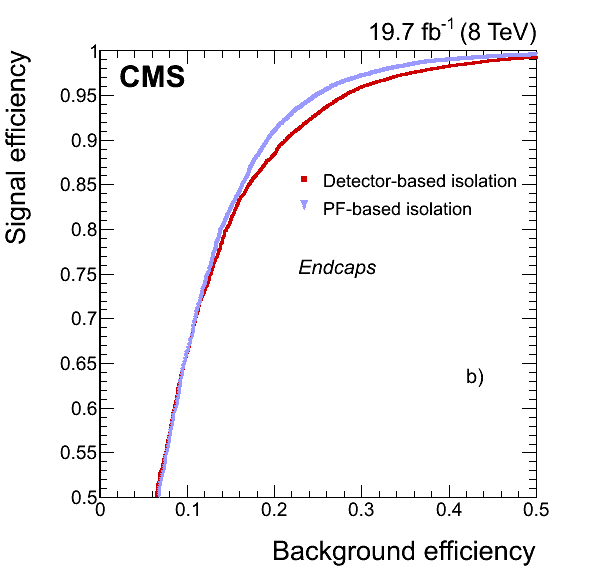
\includegraphics[width=0.4\textwidth]{chapter4/ROC_IsoOnly_Data_EE_HighPt.png}}\\
     \caption{PF electron isolation shows better performance in both EB and EE with respect to detector based isolation variable~\cite{electron_reco2015}}
     \label{fig:eleIso}
\end{figure}


This should be used for B-tagging citation~\cite{BTV-16-002}


\subsection{Tau lepton reconstruction} \label{Chapter:taureco}

In Run I CMS experiment, tau lepton are constructed with hadrons plus strips(HPS) algorithm. In general, HPS starts with PF jets which are reconstructed with $anti-k_{T}$, as the initial seeds. $\pi_{0}$ components from the $\tau$ hadronic decays are first constructed and combined with the charge hadrons parts, to identify different $\tau$ decay modes and calculate $\tau$ four-momentum and other quantities ~\cite{TauIdentiRunI}. 

Photon conversions and the bremsstrahlung of electron/positron when traveling inside the CMS detector are well treated by the HPS algorithm. These phenomenons broaden the signature of the tau decay. With PF jets as input, the algorithm constructs strips out of electromagnetic particles and starts by taking the strip in which contains the most energetic electromagnetic particle as the center one. With the center strip, a window of the size $\Delta \eta=0.05$ and $\Delta \phi=0.2$ is taken. Within this window, if other charged particles are found, they are associated with the strip. The position of the strip is taken and four momentum of the strip is calculated. This procedure is repeated, until no strips can be constructed. The selected strips are required to have $P_{T}^{strip}>1GeV$. The following decay topologies are taking into account by HPS:
\begin{enumerate}[$\bullet$]
\item one charged particle without any strip, $h^{\pm}$ and the case when $\pi^{0}$ is not energetic enough to form a strip
\item one charged particle plus one strip
\item one charged particle plus two strips
\item three charged partibles. 
\end{enumerate} 

All of the charged hadrons and strips are required to be contained in the $\Delta R=2.8/P_{T}^{\tau_{h}}$ core, where the $P_{T}^{\tau_{h}}$ is the reconstructed $\tau_{h}$ transverse momentum and $\Delta R$ is defined as $\Delta R=\sqrt(\Delta \phi^{2}+\Delta \eta^{2})$. The $\tau_{h}$ candidate is also required to match the direction of the seed PF jet within $\Delta R=0.1$. Assuming all of the charged hadrons to be pions and taking in the associated strips, the HPS algorithm requires that different decay topologies meet the intermediate meson mass as listed in Table.~\ref{tb:tauHdecay}. 

The cut based $\tau_{h}$ isolation discriminant required that the PF charged particles and photons to be considered in the isolation variable have $\pt>0.5$ GeV and within an isolation cone  $\Delta R=0.5$ in $\tau_{h}$ direction. The particles that  constituent $\tau_{h}$ are excluded from the summation. The effect of charged particle from pileup is eliminated by considering on the charged particle oriented from the $\tau_{h}$ production vertex with in $D_{z}=0.2$ cm and $\Delta r=0.03$ cm. The effect of pileup on the isolation of the photons on the strips is estimated by summing the charged particles that are not oriented from $\tau_{h}$ decay primary vertex, within $\Delta R=0.8$ cm in the direction of and have the impact parameter $D_{z}>0.2$ cm. Then a factor $\Delta \beta$ is multiplied to the $\pt$ sum. The isolation variable is defined as in Equation.~\ref{eq:taucutiso1}.

\begin{align}
I_{\tau}=\sum \pt^{\text{charged}} (d_{z}<0.2 \ \text{cm})+\text{max}(0,\sum \pt^{\gamma}-\Delta \beta \sum \pt^{\text{charged}} (d_{z}>0.2 \ \text{cm}))\label{eq:taucutiso1}
\end{align}

Tight, loose, medium working points(WP) for the tau isolation discriminants. The exact of the energy selection is suggested by the study of QCD dijet events, by requiring the $I_{\tau}$ in Equation.~{eq:taucutiso1} to have different values. The loose cut brings in approximate $1\%$ of fake $\tau$ from jets. 


\begin{table}[htp]
\caption{Dominant hadronic $\tau$ lepton decays branching fractions and the associated intermediate resonance. The h stands for both $\pi$ and K. The table is symmetric under charge conjugation.}\label{tb:tauHdecay}
\begin{center}
\begin{tabular}{|c|c|c|c|}
\hline
Decay mode                                             & Resonance & Mass ($MeV/c^{2}$) & Branching fraction(\%)\\\hline
$\tau^{-}\to h^{-}v_{\tau}$                                     &                                  &           &  11.6\%     \\
$\tau^{-}\to h^{-}\pi^{0} v_{\tau}$                       & $\rho^{-}$                 & 770     &   26.0\%      \\
$\tau^{-}\to h^{-}\pi^{0} \pi^{0}  v_{\tau}$       & $\alpha_{1}^{-}$       & 1200   &   9.5\%     \\
$\tau^{-}\to h^{-}h^{+}h^{-}v_{\tau}$                     & $\alpha_{1}^{-}$       &  1200  &   9.8\%  \\
$\tau^{-}\to h^{-}h^{+}h^{-}\pi^{0} v_{\tau}$      &                                  &            &   4.8\% \\\hline
 \end{tabular}
\end{center}
\end{table}


In CMS Run II, Tau reconstruction algorithm HPS has been improved~\cite{TauRecoandIDRunII}. The major improvement lies in Dynamic strip instead of fix size strip. Tau decay products can also affect the isolation. Charged pions in tau decay products experience nuclear interaction with tracker materials, which can results in low $P_{T}$ secondary particles. Photons from the neutral pion decay can also go through pair production into $e^{+}e{-}$, which further spread because of bremsstrahlung and the magnetic field. Broadening the strip is need in these cases in order to better cover the tau decay production. On the other hand, if the tau is boosted, high $P_{T}$ decay products tends to be more concentrate and smaller strip size will be better. Similar to RunI tau reconstruction, the algorithm starts with hightest $\pt$ charged particle as seeds for the strip. Starting from the seed strip, a window in $\eta$ and $\phi$ direction is set.  

\begin{align*}
\delta\eta&=f(P_{T}^{\gamma})+f(P_{T}^{strip})   & f(P_{T})&=0.2\cdot P_{T}^{-0.66}\\
\delta\phi&=g(P_{T}^{\gamma})+g(P_{T}^{strip}) & g(P_{T})&=0.35\cdot P_{T}^{-0.71}\\
\end{align*}

The window is determined from single $\tau$ gun MC simulation. 95\% of the decay product will be covered in that range. The upward and downward limits for $\eta$ is 0.15 and 0.05, for $\phi$ the range is 0.3 and 0.05.  The position of strip is set as $\pt$ weighted average against all of the objects. 

\begin{align*}
\eta_{strip}&=\frac{1}{P_{T}^{strip}}\cdot\sum P_{T}^{\gamma}\cdot\eta_{\gamma}\\
\phi_{strip}&=\frac{1}{P_{T}^{strip}}\cdot\sum P_{T}^{\gamma}\cdot\phi_{\gamma}\\
\end{align*}

Construct the strip until no seed strip can be found. After the construction of the $\tau$ lepton, for different decay mode, $m_{\tau}$ is required to lie in different mass windows~\cite{TauReconstuction}.  The conditions of different hadronic decay mode mass window are listed in the Table.~\ref{tb:tauHdecayRecomass}. With respect to RunI, the difference in mass window is $\delta m$, which originates from dynamic clustering. $\delta m$ is calculated as:

\begin{align*}
\delta m&=\sqrt{\Big(\frac{\partial m_{\tau}}{\partial \eta_\text{{strip}}}\cdot f(\pt^\text{{strip}})\Big)^{2}+\Big(\frac{\partial m_{\tau}}{\partial \phi_\text{{strip}}}\cdot g(\pt^\text{{strip}})\Big)^{2}}\\
\end{align*}
with:
\begin{align*}
\frac{\partial m_{\tau}}{\partial\eta_{strip}}&=\frac{P_{z}^{strip}\cdot E_{\tau}-E_{strip}\cdot P_{z}^{\tau}}{m_{\tau}}\\
\frac{\partial m_{\tau}}{\partial\phi_\text{{strip}}}&=\frac{-(P_{y}^{\tau}-P_{y}^\text{{strip}})\cdot P_{x}^\text{{strip}}+(P_{x}^{\tau}-P_{x}^\text{{strip}})\cdot P_{y}^\text{{strip}}}{m_{\tau}}
\end{align*}


\begin{table}[htp]
\caption{$\tau$ hadronic decay mode hypothesis signatures compatibility tests. $m_{\tau}$ is required to be in the mass window }\label{tb:tauHdecayRecomass}
\begin{center}
\begin{tabular}{|c|c|}
\hline
Decay mode                                             & Mass window\\\hline
$\tau^{-}\to h^{-}\pi^{0} v_{\tau}$                       & $0.3-\delta m_{\tau}<m_{\tau}<1.3\cdot \sqrt{\pt/100}+\delta m_{\tau}$      \\\hline
$\tau^{-}\to h^{-}\pi^{0} \pi^{0}  v_{\tau}$       &  $0.4-\delta m_{\tau}<m_{\tau}<1.2\cdot \sqrt{\pt/100}+\delta m_{\tau}$   \\\hline
$\tau^{-}\to h^{-}h^{+}h^{-}v_{\tau}$                     & $0.8-\delta m_{\tau}<m_{\tau}<1.5+\delta m_{\tau}$   \\\hline
 \end{tabular}
\end{center}
\end{table}

In current algorithm, $\tau^{-}\to h^{-}h^{+}h^{-}v_{\tau}$ is not included, because of the jets contamination. This hadronic $\tau$ decay mode composed of 4.8\% of total branching fraction. The $h^{-}\pi^{0}$ and $h^{-}\pi^{0}\pi^{0}$ are analyzed together, which is referred as $h^{-}\pi^{0}$.

The analysis with 2016 datasets, MVA based $\tau$ isolation criteria is used, which keeps high identification efficiency while maintains relatively low fake rate compared with cut based discriminator. A Boosted Decision Tree(BDT) has been used in the training of the isolation variable. With BDT, the isolation variable shows a good distinguishing power against jets. Various variables have been used as BDT inputs. The variables are isolation variable($I_{\tau}$), impact parameter from highest $\pt$ track of $\tau_{h}$ candidate, $\tau_{h}$ decay mode information, shape variables like $\Delta R$, $\Delta \eta$, $\tau-$lifetime information and photon electron multiplicity, more of the exact variables used are discussed in~\cite{TauRecoandIDRunII,TauReconstuction}. BDT uses these variables to distinguishing $\tau_{h}$ dacay($H \to \tau \tau$) from jets, which can be the decay products from quarks and gluons(QCD MC).  

BDT method also used in the tau discriminating again electron training. The algorithm utilizes the variables that sensitive to the energy deposit in Ecal and Hcal, the electron bremsstrahlung, overall particle multiplicity and difference in electromagnetic and hadronic showers. Detail list of variable can be find in~\cite{TauRecoandIDRunII,TauReconstuction}.

Tau signals can be faked by muons, especially in $\tau_{h}$ decay mode $h^{\pm}$. Tau against muon cut based muon discriminant is set by checking if there are signals in the muon system within $\Delta R=0.3$ of the $\tau_{h}$ direction or if the energy sum from Ecal and Hcal is less than 20$\%$ of the total $\tau$ energy. If less than two hits are found in the muon system, then it passes the loose working point. If no hits are found in the muon system, then this is the tight working point. 

\subsection{Jet reconstruction}


Anti-$k_{t}$ jet clustering algorithm~\cite{Cacciari:2008gp} is used in CMS for the jet reconstruction. The algorithm starts by introducing the distance $d_{ij}$ and $d_{iB}$ as following,

\begin{align*}
d_{ij}&=min(k_{ti}^{2p},k_{tj}^{2p})\frac{\Delta_{ij}^{2}}{R^{2}}\\
d_{iB}&=k_{ti}^{2p}
\end{align*}

$d_{ij}$ is the distance between entities, the particle and the pseudojet. $\Delta_{ij}$ is the difference of rapidity and azimuth between entry i and entry j. $\Delta_{ij}^{2}=(\eta_{i}-\eta_{j})^{2}+(\phi_{i}-\phi_{j})^{2}$. R is a radius parameter. $k_{ti}$ and $k_{tj}$ stands for the momentum of the entries respectively. p is a parameter used to specify jet construction algorithms.  For Anti-$k_{t}$, p=-1. $d_{iB}$ is the distance between entry i and the beam. If the parameter p is set for other values, for example p=1 or 0, then the algorithm is the $k_t$~\cite{ktalgo} or Cambridge/Aachen jet reconstruction algorithm~\cite{Aachenjetalgo}.  With the Anti-$k_{t}$, assuming in one event, there are a couple hard particle with high momentum, $k_{t1}$, $k_{t2}$ and so on, also large numbers of soft ones around. Starting from $k_{t1}$ as an example, if $d_{1j}$ is smaller, then entry j combined with entry 1, if $d_{1B}$ is smaller, then entry 1 is set as a jet and removed from the list. The soft entries tend to ground around the high momentum entries to the range $\Delta_{ij}= R$, if there is no other hard entry around. If two hard entries are within the distance R, then the two entries are clustered into a single entry. In this case, if $k_{1}\gg k_{2}$, then the center is more closed to jet 1. If $k_{1}\sim k_{2}$, the boundary between to two jets is defined by $\Delta R_{1b}/k_{t1}=\Delta_{2b}/k_{t2}$. Jet clustering continues until all of the jets are clustered in the events. 

Jet energy is corrected to have the correct energy scale.  The correction goes through a couple of steps~\cite{jetenergycorrection}. The major corrections are derived from simulated samples and the residual corrections from the different response between MC and data are from data-driven methods. 

Pileup events can increase the measured jet energy, especially in LHC Run II, the number of pileup per event doubled. Two types of pileup affect the performance the most, in-time pileup(IT PU) and out-of time pileup(OOT PU). The IT PU refers to the additional events produced by the proton-proton collision within the same bunch-crossing as the primary hard collision.   The OOT PU refers to the events that produced in previous bunch crossing or subsequent one that affect current bunch. OOT PU can be mitigated by explore the timing window, pulse shape of the calorimeter. The IT PU mitigation is mainly discussed. Charged hadrons from IT PU in CMS are removed with Charged-hadron subtraction(CHS) algorithm in CMS. Tracks with the vertexes that are identified from PU with charged particles inside are removed. CHS removes around 50\% of the IT PU within the tracker coverage region. There are also soft jets from pileup interaction. These jets are usually in low energy range and affects the JES by overlapping with the hard jets. Multivariate analysis(MVA) with inputs from jet shape and jet constitution information can more than 90\% of pileup jets. This MVA ID is referred as PUJetID~\cite{PU_jetID}. After rejecting the charged particle jets and soft jets from pileup, a jet area method~\cite{FastJetalso} is used to further eliminate the effects from PU. In this method, an estimated energy density bringing in by the PU and effective area of jet is used to calculate the offset energy. After the PU correction, a matching between particle-level jets and reconstructed jets is performed with MC samples for the simulated response corrections. 









\section{Event simulation}


%
% Chapter 5 
%



%% I need to describe muon ID in chaper 4.2 and Tau decay mode finding, tau MVA ID around 4.2 too 
\chapter{LFV event selection}
In both 8 TeV $H\rightarrow e\tau_h$ and 13 TeV $H\rightarrow\mu\tau_h$ analyses, events are selected in several steps. A loose selection selects on the different IDs, energy, geometry parameters of the analysis related objects. In the $\mcol$ fit analysis this is followed by a tighter set of selection criteria in which selection requirements are placed on the kinematics variables and fits on variable $\mcol$ in both  $H\rightarrow e\tau_h$ and $H\rightarrow\mu\tau_h$ analysis. This selection sequence is referred as $\mcol$ fit analysis. In $H\rightarrow\mu\tau_h$, there is an alternate selection sequence that follows the loose selection. A multivariate analysis with a Boosted decision tree (BDT) is defined and fits on the BDT discriminator. This is referred as the BDT fit analysis and provides more sensitive results in $\Hmuhad$ analysis. 



\section{\texorpdfstring{$H\rightarrow\mu\tau_h$}{Lg}}
\subsection{Loose selection}
Tau leptons from signal events decay hadronically. A SM Higgs boson is much heavier than its decay products $\mu$ and $\tau$. The $\mu$ and $\tau$ leptons are expected to have high $P_{T}$. As the decay products from signal events are boosted, therefore a cut on $\Delta R=\sqrt(\Delta phi^{2}+\Delta eta^{2})$, $\Delta R>0.3$ is applied. The $\mu$ and $\tau$ candidates are required to have opposite sign of charge as the Higgs boson is neutral. Further, events with additional $\mu$ and $\tau$ that pass the loose selection and events with jets that are identified by the combined secondary vertex b-tagging algorithm \cite{btag_ago} as a b quark jets are vetoed. The high level trigger used in the analysis selects isolated muons that have energy higher than 24 GeV at HLT level. A further $P_{T}$ cut on the reconstructed $\mu$,  $P_{T}>26$ GeV and $|\eta|<2.4$ are required. Muons are required to pass the recommended Medium muon ID and tight cut based isolation $I^{\mu}_{rel}<0.15$, which refers to the PF muon isolation variable and is computed as shown in Equation.~\ref{Iso_correction}. %For the LHC data 2016, running period BCDEF, ICHEP medium muon ID is applied(table~\ref{tbl:ICHEPMedID}), for data running period G and H, also the monte Carlo samples, standard medium muon ID(table~\ref{tbl:standardMedID})are applied to achieve the best performance for muon identification.

Hadronic taus are required to have $P_T>30$ GeV,$|\eta|<2.3$, passing old tau decay mode finding, the MVA based tight tau isolation ID and tau discriminators against electrons and muons. %The discriminators are very loose MVA based rejection against electrons and cut-based tight rejection against muons.  


Events in the analysis are divided into four categories based on the number of jets. In 2-jets category, it is furthered divided into 2 categories,  2-jet gluon gluon fusion higgs production(ggH) category and 2-jet vector boson fusion(VBF) category based on the value of 2 jets invariant mass($M_{jj}$). The ggH and VBF Higgs production models are considered in the analysis. This choice of categorization enhanced one of the production models in each of the categories and improves the sensitivity. The 0-jet category enhances ggH production mode. In 1-jet category, the dominant signal production mode is also ggH, but with a boosted jet associated with the production and VBF higgs production also contributes this category. In the 2-jet ggH category, signal events mainly come from ggH, while in 2-jet VBF, VBF higgs is the dominant production channel.  The following is a more detailed list of the selection condition in each categories.

\begin{enumerate}
\item[{\bf 0-jet:}] No events have jets pass the loose PF ID and  with jet $P_T>30$ GeV, $|\eta|<4.7$.
\item[{\bf 1-jet:}] Events with one jet passes losse PF ID and jet $P_T>30$ GeV, $|\eta|<4.7$.
\item [{\bf 2-jets ggH:}] Events have two jets passing loose PF ID, $P_T>30$ GeV, $|\eta|<4.7$ and a requirement on the invariant mass of the two jets, $\textrm{M}_{jj}<550$ GeV. 
\item [{\bf 2 jets VBF:}] Events with two jets pass loose PF ID. Jets $P_T>30$ GeV, $|\eta|<4.7$ and $\textrm{M}_{jj}>550$ GeV are required. 
\end{enumerate} The threshold on $\textrm{M}_{jj}$ has been optimized to give the best expected exclusion limits.


\subsection{Cut-based analysis}
After the loose selection and the categorization, a further cut-based selection is applied. Variables that can help distinguish signal from background are $P_{T}^{\mu}$, $P_{T}^{\tau}$ and $M_{T}(\tau_{h})$. The lepton $P_{T}$ variables are very powerful background discriminant variables, but will also cause the problem that signal peaks under backgrounds. As leptons from signal process  tend to have higher $P_{T}$ values, cutting tighter on the lepton $P_{T}$, removes more background events. However this will also reshape some of the backgrounds, making them peak closer under the signal so that signal processes will be affected more by the background statistics fluctuation. In the $H\rightarrow e\tau_h$ analysis, the effect of cutting tighter on lepton $P_{T}$ will be shown. In $H\rightarrow\mu\tau_h$ search, lepton $P_{T}$ variables are kept at loose values and optimized on other variables to achieve tighter expected limits. 

The optimization is procedure uses only Monte Carlo samples so as not to double use data. In $\Hmuhad$  channel, the variables tuned are $\textrm{M}_{jj}$ and $M_{T}(\tau_{h})$. The selection criteria has been optimized to have the most stringent expected limits with the Asimov dataset(background only). The name Asimov dataset is inspired by the short story Franchise, by Isaac Asimov. If looser values of the cuts give the same expected limits as the tighter ones, then the looser cut values are chosen to have more statistics. Examples of optimization by checking the limits are shown in Figure. \ref{fig:optMT} and~\ref{fig:optVBFmass}, in which the optimization of $M_T(\tau_{h})$  and $\textrm{M}_{jj}$ are shown. A full summary of the cuts optimized for $\Hmuhad$ is shown in Table.~\ref{tab:Mhadcategories}


\begin{figure}[htbp] 
     \centering
     \subfigure[0 jet]{ \includegraphics[width=0.4\textwidth]{chapter5/Tuning/ggtMtToPfMet_type1.pdf}}
     \subfigure[1 jet]{ \includegraphics[width=0.4\textwidth]{chapter5/Tuning/boosttMtToPfMet_type1.pdf}}\\
     \subfigure[2 jets, gg-enriched]{ \includegraphics[width=0.4\textwidth]{chapter5/Tuning/vbf_ggtMtToPfMet_type1.pdf}}
     \subfigure[2 jets, VBF-enriched]{ \includegraphics[width=0.4\textwidth]{chapter5/Tuning/vbf_vbftMtToPfMet_type1.pdf}}
     \caption{Expected limits based on an Asimov dataset as a function of $M_T(\tau, MET)$ for the different categories.}
     \label{fig:optMT}
\end{figure}

\begin{figure}[!tbp] 
\centering
\includegraphics[width=0.4\textwidth]{chapter5/Tuning/vbf_vbfvbfMass.pdf}
\caption{Expected limits based on an Asimov dataset as a function of $M_{jj}$ for the 2 jet categories.}
\label{fig:optVBFmass}
\end{figure}



\begin{table}[hbtp]
  \begin{center}
  \caption{Selection criteria in each category with the optimization of the $\Hmuhad$ analysis}
  \begin{tabular}{l} \hline
  {\bf 0-jet category} \\ \hline
  \tabitem $\pt^{\mu}>26$ GeV, $\pt^{\tau}>30$ GeV\\
  \tabitem $M_T(\tau)<105$ GeV \\
  \tabitem No jets with $\pt^{jet}>30$ GeV, $|\eta|<4.7$, LooseID \\ \hline
 {\bf 1-jet category} \\ \hline
  \tabitem $\pt^{\mu}>26$ GeV, $\pt^{\tau}>30$ GeV \\
  \tabitem $M_T(\tau)<105$ GeV \\
  \tabitem One jet  with $\pt^{jet}>30$ GeV, $|\eta|<4.7$, LooseID
  \\ \hline
  {\bf 2-jet, gg-enriched category} \\ \hline
  \tabitem $\pt^{\mu}>26$ GeV, $\pt^{\tau}>30$ GeV \\
  \tabitem $M_T(\tau)<105$ GeV \\
      \tabitem $\pt^{jet1}>30$ GeV,$\pt^{jet2}>30$ GeV
      $|\eta_{jet1}|<4.7$,$|\eta_{jet2}|<4.7$, LooseID\\
      \tabitem $M_{jj}<550$ GeV\\
      \tabitem Two jets with $\pt^{jet}>30$ GeV, $|\eta|<4.7$, LooseID\\ \hline
  {\bf 2-jet, VBF-enriched category} \\ \hline
  \tabitem $\pt^{\mu}>26$ GeV, $\pt^{\tau}>30$ GeV \\
  \tabitem $M_T(\tau)<85$ GeV \\
      \tabitem $\pt^{jet1}>30$ GeV,$\pt^{jet2}>30$ GeV
      $|\eta_{jet1}|<4.7$,$|\eta_{jet2}|<4.7$, LooseID\\
      \tabitem $M_{jj}>550$ GeV\\
      \tabitem Two jets with $\pt^{jet}>30$ GeV, $|\eta|<4.7$, LooseID\\ \hline
  \label{tab:Mhadcategories}
\end{tabular}
\end{center}
\end{table}




\subsection{Multivariate analysis}
A boosted decision trees(BDT) method is used as the multivariate analysis method in the $H\rightarrow\mu\tau_h$ search which is more sensitive than the $\mcol$ fit analysis. The BDT algorithm used in this search is implemented in the TMVA package \cite{TMVAnote}. BDT takes in signal and background datasets with a selected set of input variables. Input variables are the ones that show distinguishing power between signal and backgrounds. The training output is a weight file, which contains a list of weights to indicate how likely an event is signal-like with a give set of input variables. A more detail description of the BDT method is available in section \ref{BDTchaper}.  In this analysis, signal and background events are required to pass the loose selection criteria. All of the categories are combined. The signal events from the ggH and VBF Higgs production mode are mixed by weighting with respect to their production cross section. The background sample used in the training is the misidentified lepton background from the like sign region(Region II as in Table.~\ref{tab:fakeratediagram}). The list of BDT input variables  is in the following list and the distribution of the variables are shown in Fig.~\ref{fig:BDT_input_var_mutauhad}.

\begin{itemize}
\item Transverse mass between the $\tauh$ and $\ETmiss$, $M_{T}(\tau_{h})$.
\item Missing transverse energy, $\ETmiss$.
\item Pseudorapidity difference between the $\mu$ and the $\tauh$ candidate, $\Delta\eta(\mu, \tauh)$.
\item Azimutal angle between the $\mu$ and the $\tauh$, $\Delta\phi (\mu,\tauh)$.
\item Azimutal angle between the $\tauh$ and the $\ETmiss$, $\Delta\phi(\tau_h,\ETmiss)$.
\item Collinear mass, $\mcol$.
\item Muon $\pt$.
\item $\tau_h$ $\pt$.
\end{itemize}

\begin{figure}[htpb]\centering
 \includegraphics[width=0.315\textwidth]{chapter5/BDTvariable/LFV_preselection_collMass_type1_Fakes_PoissonErrors.pdf}
 \includegraphics[width=0.315\textwidth]{chapter5/BDTvariable/LFV_preselection_mPt_Fakes_PoissonErrors.pdf} \\
 \includegraphics[width=0.315\textwidth]{chapter5/BDTvariable/LFV_preselection_tPt_Fakes_PoissonErrors.pdf}
 \includegraphics[width=0.315\textwidth]{chapter5/BDTvariable/LFV_preselection_tMtToPfMet_type1_Fakes_PoissonErrors.pdf}  \\
 \includegraphics[width=0.315\textwidth]{chapter5/BDTvariable/LFV_preselection_tDPhiToPfMet_type1_Fakes_PoissonErrors.pdf}
 \includegraphics[width=0.315\textwidth]{chapter5/BDTvariable/LFV_preselection_type1_pfMetEt_Fakes_PoissonErrors.pdf} \\
 \includegraphics[width=0.315\textwidth]{chapter5/BDTvariable/LFV_preselection_m_t_DPhi_Fakes_PoissonErrors.pdf}
 \includegraphics[width=0.315\textwidth]{chapter5/BDTvariable/LFV_preselection_m_t_DEta_Fakes_PoissonErrors.pdf}
\caption{Distributions of the  input variables to the BDT for the \Hmuhad channel.}
 \label{fig:BDT_input_var_mutauhad}
\end{figure}


\begin{figure}[htbp] 
     \centering
     \subfigure[Signal sample variables correlation]{ \includegraphics[width=0.4\textwidth]{chapter5/CorrelationMatrixS.pdf}}
     \subfigure[Background sample variable correlation]{ \includegraphics[width=0.4\textwidth]{chapter5/CorrelationMatrixB.pdf}}\\
     \caption{Expected limits based on an Asimov dataset as a function of $M_T(\tau, MET)$ for the different categories.}
     \label{fig:BDTvarcorrelation}
\end{figure}


The chosen input variables show low correlation in both samples as shown in Figure.~\ref{fig:BDTvarcorrelation}. In the training process, overtraining needs to be carefully treated. The overtraining problem refers to the case that the classifier between signal and background samples are specific to the particular training sample used. The training recognizes the specific features that only occurs in the training samples. Most of the time, these features are caused by the limited number of training events or with the same number of events, too many variables with weak distinguishing power are used. The overtraining checks is performed by checking with the testing samples to see if similar distinguishing power can be achieved with the output weight file from the training samples. Training and testing samples show good agreement and the training process exempts from overtraining as indicated in Figure.~\ref{fig:BDTovertraining}.
\begin{figure}[htbp] 
\centering
\includegraphics[width=0.6\textwidth]{chapter5/overtrain_BDT.pdf}
\caption{Overtraining checking for the BDT training in the TMVA package.}
\label{fig:BDTovertraining}
\end{figure}

\section{\texorpdfstring{$H\rightarrow e \tau_h$}{Lg}}

\subsection{Loose selection}
In $ \Hehad$ channel, the high level trigger that is used applies an electron $\pt$ cut at 27 GeV at HLT level. A further cut on electron $P_{T}>30$ GeV is applied. Electrons are also required to have $|\eta_{e}<2.3|$ and $D_{z}<0.2 cm$. $D_{z}$ is the longitudinal impact parameter that shows the displacement between primary vertex and track path. Electrons are required to pass the MVA based tight ID and cut based PF tight isolation  $I_{rel}^{e}<0.1$. Tau candidates are required to have $P_{T}>30$ GeV, pseudorapidity $|\eta^{\tau}<2.3|$ and the longitudinal impact parameter $D_{z}<0.2$ cm. Tau isolation used is the cut based tight tau isolation. In addition, tau candidates are required to pass the tau Decay mode finding and tau discriminator against electrons and muons. The analysis also requires no extra isolated electrons with $\pt>10$ GeV and extra taus with $\pt>20$ GeV. Tau and electron candidates are required to have opposite sign of charges and separate with $\Delta R>0.4$ from any jets in the events with $\pt>30$ GeV. All of the requirements contribute to the selections of good qualities candidates. The datasets are binned into three categories according to the number of jets in the events:
\begin{enumerate}
\item[{\bf 0-jet:}] No events have jets pass the loose PF ID and  with jet $P_T>30$ GeV, $|\eta|<4.7$. This category enhances the gluon-gluon fusion contribution.
\item[{\bf 1-jet:}] Events with one jet passes loose PF ID and jet $P_T>30$ GeV , $|\eta|<4.7$. This category enhances the gluon-gluon fusion production with initial state radiation.
\item [{\bf 2 jets:}] Events with two jets pass loose PF ID and with jet $P_T>30$ GeV and $|\eta|<4.7$, This category contains both Higgs production mode and with an enhancement in VBF production mode. \end{enumerate}

With the preselection and binning of the jets numbers, the $\mcol$ distribution of $\Hehad$ in different categories are shown in Figure.~\ref{fig:etauCol_preselection}
\begin{figure}[hbtp]\centering
 \subfigure[0 jet]{\includegraphics[width=0.4565\textwidth]{chapter5/etauPlots/etau_preselection0jet.pdf}}
 \subfigure[1 jet]{ \includegraphics[width=0.4565\textwidth]{chapter5/etauPlots/etau_preselection1jet.pdf}}
 \subfigure[2 jets]{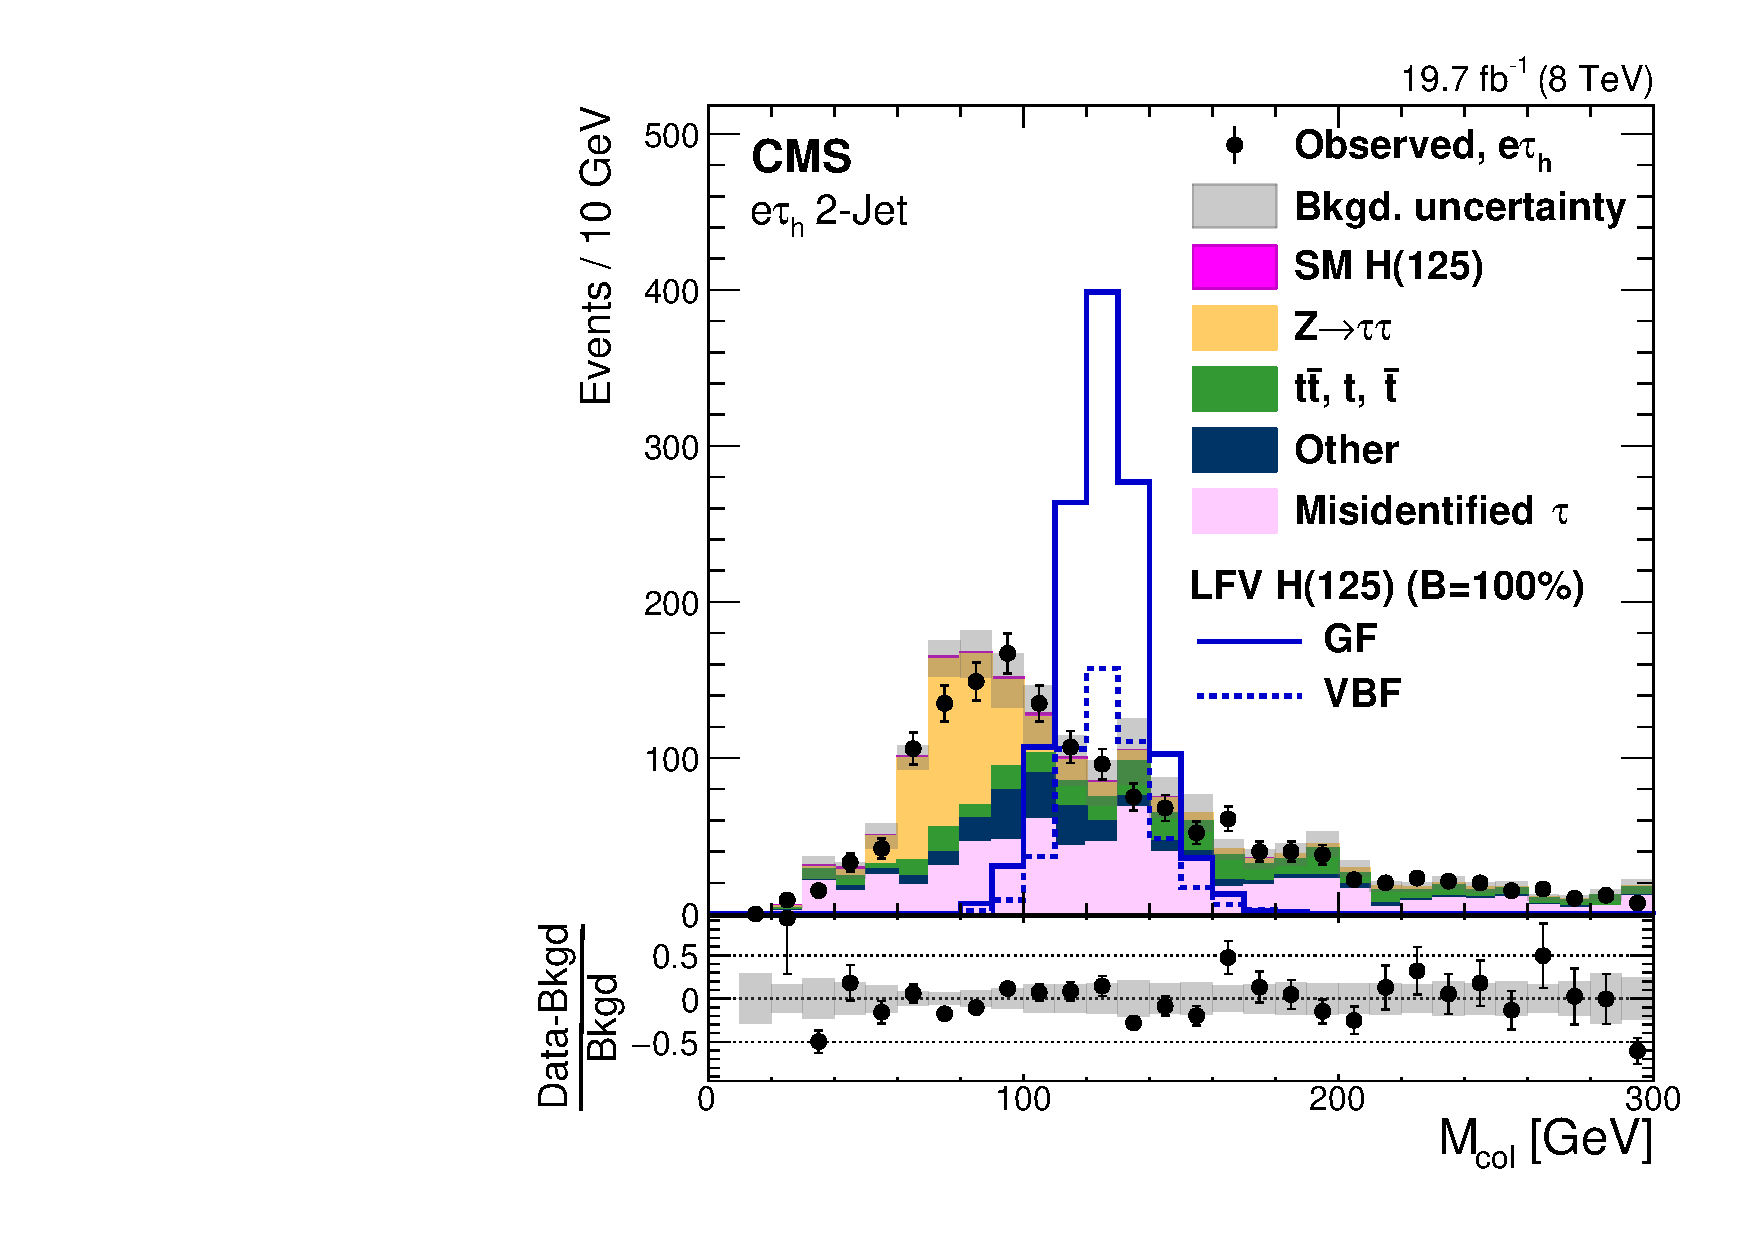
\includegraphics[width=0.4565\textwidth]{chapter5/etauPlots/etau_preselection2jet.pdf}}
 \caption{With loose selection conditions, the comparison of the observed collinear mass distributions with background from prediction. The shaded grey bands indicate the total background uncertainty.
The open histograms correspond to the expected signal distributions for $\mathcal{B}(\Hehad)=100\%$ in the  0-jet, 1-jet and 2-jet categories, respectively.}
\label{fig:etauCol_preselection}\end{figure}


\subsection{Cut-based analysis}
A set of kinematics variables are used to further select signal events. In $\Hehad$ channel, similar to the $\Hmuhad$, muon and tau leptons from the signal events are highly boosted so as $\pt$ variables play an important role in distinguishing from background events and the separation in $\phi$ direction is bigger between $\mu$ and $\tau$ of signal events. The variable $M_{T}(\tau_{h})$ which is the transverse mass form by the reconstructed $\tau$ and MET is also used in the selection. In the two jets category, the invariant mass of two jets $M_{jj}$ is used as a cut variable.  The cuts have been optimized to have the most stringent expected limits with the Asimov dataset. The detailed cuts used for $\Hehad$ is shown in table.~\ref{tab:ehadcategories}.


\begin{table}[hbtp]
  \begin{center}
  \caption{Selection criteria for each event category after cut
    optimization, for the $\Hehad$ channel}
  \begin{tabular}{l} \hline
  {\bf 0-jet category} \\ \hline
  \tabitem $\pt^{e}>45$ GeV, $\pt^{\tau}>30$ GeV, $\Delta \phi_{e \tau}>2.3$ \\
  \tabitem $M_T(\tau)<70$ GeV \\
  \tabitem No jets with $\pt^{jet}>30$ GeV, $|\eta|<4.7$, LooseID \\ \hline
 {\bf 1-jet category} \\ \hline
  \tabitem $\pt^{e}>35 $GeV, $\pt^{\tau}>40$ GeV \\
  \tabitem One jet  with $\pt^{jet}>30$ GeV, $|\eta|<4.7$, LooseID
  \\ \hline
  {\bf 2-jet category} \\ \hline
  \tabitem $\pt^{e}>35$ GeV, $\pt^{\tau}>30$ GeV \\
  \tabitem $M_T(\tau)<50$ GeV \\
      \tabitem $\pt^{jet1}>30$ GeV,$\pt^{jet2}>30$ GeV
      $|\eta_{jet1}|<4.7$,$|\eta_{jet2}|<4.7$, LooseID\\
      \tabitem $\Delta\eta(jet1,jet2)>2.3$\\
      \tabitem $M_{jj}>400$ GeV\\
      \tabitem Two jets with $\pt^{jet}>30$ GeV, $|\eta|<4.7$, LooseID \\ \hline
  \label{tab:ehadcategories}
\end{tabular}
\end{center}
\end{table}












%
% Chapter 6 
%

%
% Chapter 6
%

%% I need to describe muon ID in chaper 4.2 and Tau decay mode finding, tau MVA ID around 4.2 too 
\chapter{LFV event selection}
For both 8TeV analysis $H\rightarrow e\tau_h$ channel and 13TeV analysis  $H\rightarrow\mu\tau_h$, events are selected in several steps. The loose selection on the different IDs, energy, geometry parameters of the analysis related objects are applied. In both  $H\rightarrow e\tau_h$ and $H\rightarrow\mu\tau_h$ analysis, cut-based analyses are applied. In $H\rightarrow\mu\tau_h$, a multivariate analysis with Boosted decision tree (BDT) is exploited to provide more sensitive results. 



\section{\texorpdfstring{$H\rightarrow\mu\tau_h$}{Lg}}
\subsection{Loose selection}
In $H\rightarrow\mu\tau_h$ events, tau leptons from signal events decay hadronically. SM higgs is much heavier than the LFV decay products $\mu$ and $\tau$, so $\mu$ and $\tau$ are expected to have high $P_{T}$. Since the decay products are boosted, a cut on the $\Delta R>0.3$ is applied. $\Delta$R is defined as $\Delta R=\sqrt(\Delta phi^{2}+\Delta eta^{2})$. Higgs has no charge, so $\mu$ and $\tau$ candidates are required to have opposite sign of charges. Further, the events with additional $\mu$ and $\tau$ that pass a loose selection, the events with jets that are identified by the combined secondary vertex(CSVv2) b-tagging algorithm \cite{btag_ago} as a b quark jets will be vetoed. Muons from signal events are boosted and isolated, as mentioned in previous chapter, the trigger HLT\_IsoMu24 or HLT\_IsoTkMu24 is used. The trigger select isolated muons that have energy higher than 24GeV. An further $P_{T}$ cut on reconstructed $\mu$,  $P_{T}>26$GeV and $|\eta|<2.4$ are applied. Muons are required to pass the recommended Medium muon ID(chapter 4.2). For the LHC data 2016, running period BCDEF, ICHEP medium muon ID is applied(table~\ref{tbl:ICHEPMedID}), for data running period G and H, also the monte Carlo samples, standard medium muon ID(table~\ref{tbl:standardMedID})are applied to achieve the best performance for muon identification.

Hadronic taus are required to have $P_T>30$GeV,$|\eta|<2.3$, passing old tau decay mode finding(chapter 4.2), an MVA based tight tau isolation ID(Chapter 4.2) and tau discriminators against electrons and muons. These discriminators are very loose MVA based rejection against electrons and cut-based tight rejection against muons.  



Events in the analysis are divided into four categories based on the number of jets in an event. In 2-jets category, it is furthered divided into 2 categories,  2-jet gluon gluon fusion higgs production(ggH) category and 2-jet vector boson fusion(VBF) category based on the value of 2 jets invariant mass($M_{jj}$) . In 0-jet category, the signal mainly comes from ggH. In 1-jet category, the dominant signal production mode is also ggH, but with a boosted jet associated with the production, some of the VBF higgs signal also shows up in this category. In the 2-jet ggH category, signal evens mainly come from ggH and in 2-jet VBF, VBF production dominants the production mode.  The following is a more detailed list of the selection condition in each categories.

\begin{enumerate}
\item[{\bf 0-jet:}] No events have jets pass the loose PF ID and  with jet $P_T>30$ GeV, $|\eta|<4.7$.
\item[{\bf 1-jet:}] Events with one jet passes losse PF ID and jet $P_T>30$ GeV, $|\eta|<4.7$.
\item [{\bf 2-jets ggH:}] Events have two jets passing loose PF ID, $P_T>30$ GeV, $|\eta|<4.7$ and a requirement on the invariant mass of the two jets, $\textrm{M}_{jj}<550GeV$. 
\item [{\bf 2 jets VBF:}] Events with two jets pass loose PF ID. Jets $P_T>30$ GeV, $|\eta|<4.7$ and $\textrm{M}_{jj}>550 GeV$ are required. 
\end{enumerate} The threshold on $\textrm{M}_{jj}$ has been optimized to give the best expected exclusion limits.


\subsection{Cut-based analysis}
With the loose selection, including the categorization, a further cut-based selection strategy is applied. Variables that can help distinguish signal from background used in this analysis are $P_{T}^{\mu}$, $P_{T}^{\tau}$ and $M_{T}(\tau_{h})$. The lepton $P_{T}$ variables are very powerful background discriminant variables, but it will also cause the problem that signal picks under the background. Leptons from signal process  incline to have higher $P_{T}$ values, by cutting tighter on the lepton $P_{T}$, more background events can be removed. However this will also reshape some of the backgrounds, making them peak closer under the signal so that signal processes will be affected more by the background statistics fluctuation. In the $H\rightarrow e\tau_h$ analysis, the effect of cutting hard on lepton $P_{T}$ will be shown. So in $H\rightarrow\mu\tau_h$ search, lepton $P_{T}$ variables are kept at loose values and tune on other variables to achieve better signal significance. 

Tuning process is done only with Monte Carlo samples to not double use data. The final results are extract from data, so the double use of data may cause biases on the results. Misidentified lepton background estimated with full data driven method, is replaced with the semi data driven estimation in tuning. In $\Hmuhad$  channel, the variables tuned are $\textrm{M}_{jj}$ and $M_{T}(\tau_{h})$. Cuts have been optimized to have the most stringent expected limits with the Asimov dataset. If loose value of the cut gives same expected limits as the tight one, then chose the loose cut value to have more statistics. Examples of obtaining the limits are shown in Fig. \ref{fig:optMT}, $M_T(\tau_{h})$ for the different categories and Fig.~\ref{fig:optVBFmass}  for the optimization of $\textrm{M}_{jj}$ in 2-jets categories. With this method and criteria, the cut optimized for $\Hmuhad$ is shown in Table.~\ref{tab:Mhadcategories}


\begin{figure}[htbp] 
     \centering
     \subfigure[0 jet]{ \includegraphics[width=0.4\textwidth]{chapter6/Tuning/ggtMtToPfMet_type1.pdf}}
     \subfigure[1 jet]{ \includegraphics[width=0.4\textwidth]{chapter6/Tuning/boosttMtToPfMet_type1.pdf}}\\
     \subfigure[2 jets, gg-enriched]{ \includegraphics[width=0.4\textwidth]{chapter6/Tuning/vbf_ggtMtToPfMet_type1.pdf}}
     \subfigure[2 jets, VBF-enriched]{ \includegraphics[width=0.4\textwidth]{chapter6/Tuning/vbf_vbftMtToPfMet_type1.pdf}}
     \caption{Expected limits based on an Asimov dataset as a function of $M_T(\tau, MET)$ for the different categories.}
     \label{fig:optMT}
\end{figure}

\begin{figure}[!tbp] 
\centering
\includegraphics[width=0.4\textwidth]{chapter6/Tuning/vbf_vbfvbfMass.pdf}
\caption{Expected limits based on an Asimov dataset as a function of $M_{jj}$ for the 2 jet categories.}
\label{fig:optVBFmass}
\end{figure}



\begin{table}[hbtp]
  \begin{center}
  \caption{Selection criteria for each event category after cut
    optimization, for the $\Hmuhad$ channel}
  \begin{tabular}{l} \hline
  {\bf 0-jet category} \\ \hline
  \tabitem $\pt^{\mu}>26GeV$, $\pt^{\tau}>30GeV$\\
  \tabitem $M_T(\tau)<105GeV$ \\
  \tabitem No jets with $\pt^{jet}>30 GeV$, $|\eta|<4.7$, LooseID \\ \hline
 {\bf 1-jet category} \\ \hline
  \tabitem $\pt^{\mu}>26GeV$, $\pt^{\tau}>30GeV$ \\
  \tabitem $M_T(\tau)<105GeV$ \\
  \tabitem One jet  with $\pt^{jet}>30 GeV$, $|\eta|<4.7$, LooseID
  \\ \hline
  {\bf 2-jet, gg-enriched category} \\ \hline
  \tabitem $\pt^{\mu}>26GeV$, $\pt^{\tau}>30GeV$ \\
  \tabitem $M_T(\tau)<105GeV$ \\
      \tabitem $\pt^{jet1}>30 GeV$,$\pt^{jet2}>30 GeV$
      $|\eta_{jet1}|<4.7$,$|\eta_{jet2}|<4.7$, LooseID\\
      \tabitem $M_{jj}<550GeV$\\
      \tabitem Two jets with $\pt^{jet}>30 GeV$, $|\eta|<4.7$, LooseID\\ \hline
  {\bf 2-jet, vbf-enriched category} \\ \hline
  \tabitem $\pt^{\mu}>26GeV$, $\pt^{\tau}>30GeV$ \\
  \tabitem $M_T(\tau)<85GeV$ \\
      \tabitem $\pt^{jet1}>30 GeV$,$\pt^{jet2}>30 GeV$
      $|\eta_{jet1}|<4.7$,$|\eta_{jet2}|<4.7$, LooseID\\
      \tabitem $M_{jj}>550GeV$\\
      \tabitem Two jets with $\pt^{jet}>30 GeV$, $|\eta|<4.7$, LooseID\\ \hline
  \label{tab:Mhadcategories}
\end{tabular}
\end{center}
\end{table}




\subsection{Multivariate analysis}
A Boost decision trees(BDT) method is chosen as the multivariate analysis method used in  $H\rightarrow\mu\tau_h$ search. It provides better sensitivity compared with the cut-based analysis. In this analysis, the BDT is provided by the TMVA package \cite{TMVAnote}. BDT method takes in signal and background datasets with a selected set of input variables. Input variables are the ones that show distinguishing power between signal and background.  The training output is a weight file, which contains a list of weights to indicate in percentage how likely an event is signal like with a give set of input variable values from that event. A more detail description of the BDT method is available in section \ref{BDTchaper}.  In this analysis, signal and background events are required to pass the loose selection criteria. All of the categories are combined. The signal events from gluon gluon fusion and vector boson fusion higgs production mode are mix by the weight with respect to their production cross section. The background sample used in the training is misidentified lepton background from the like sign region(Region II as in table **). The list of BDT input variables  is following and the distribution of the variables are shown in Fig.~\ref{fig:BDT_input_var_mutauhad}.

\begin{itemize}
\item Transverse mass between the $\tauh$ and $\ETmiss$, $M_{T}(\tau_{h})$.
\item Missing transverse energy, $\ETmiss$.
\item Pseudorapidity difference between the $\mu$ and the $\tauh$ candidate, $\Delta\eta(\mu, \tauh)$.
\item Azimutal angle between the $\mu$ and the $\tauh$, $\Delta\phi (\mu,\tauh)$.
\item Azimutal angle between the $\tauh$ and the $\ETmiss$, $\Delta\phi(\tau_h,\ETmiss)$.
\item Collinear mass, $\mcol$.
\item Muon $\pt$.
\item $\tau_h$ $\pt$.
\end{itemize}

\begin{figure}[htpb]\centering
 \includegraphics[width=0.315\textwidth]{chapter6/BDTvariable/LFV_preselection_collMass_type1_Fakes_PoissonErrors.pdf}
 \includegraphics[width=0.315\textwidth]{chapter6/BDTvariable/LFV_preselection_mPt_Fakes_PoissonErrors.pdf} \\
 \includegraphics[width=0.315\textwidth]{chapter6/BDTvariable/LFV_preselection_tPt_Fakes_PoissonErrors.pdf}
 \includegraphics[width=0.315\textwidth]{chapter6/BDTvariable/LFV_preselection_tMtToPfMet_type1_Fakes_PoissonErrors.pdf}  \\
 \includegraphics[width=0.315\textwidth]{chapter6/BDTvariable/LFV_preselection_tDPhiToPfMet_type1_Fakes_PoissonErrors.pdf}
 \includegraphics[width=0.315\textwidth]{chapter6/BDTvariable/LFV_preselection_type1_pfMetEt_Fakes_PoissonErrors.pdf} \\
 \includegraphics[width=0.315\textwidth]{chapter6/BDTvariable/LFV_preselection_m_t_DPhi_Fakes_PoissonErrors.pdf}
 \includegraphics[width=0.315\textwidth]{chapter6/BDTvariable/LFV_preselection_m_t_DEta_Fakes_PoissonErrors.pdf}
\caption{Distributions of the  input variables to the BDT for the \Hmuhad channel.}
 \label{fig:BDT_input_var_mutauhad}
\end{figure}


\begin{figure}[htbp] 
     \centering
     \subfigure[Signal sample variables correlation]{ \includegraphics[width=0.4\textwidth]{chapter6/CorrelationMatrixS.pdf}}
     \subfigure[Background sample variable correlation]{ \includegraphics[width=0.4\textwidth]{chapter6/CorrelationMatrixB.pdf}}\\
     \caption{Expected limits based on an Asimov dataset as a function of $M_T(\tau, MET)$ for the different categories.}
     \label{fig:BDTvarcorrelation}
\end{figure}


Fig.~\ref{fig:BDTvarcorrelation} shows BDT input variables in the signal and background training samples. The chosen input variables show low correlation in both samples. Fig.~\ref{fig:BDTovertraining} shows the TMVA overtraining checks. Training samples are divided into two groups, one for training and one for testing. After the training, the algorithm applies the training output to the testing sample to check if they are in good matching.

\begin{figure}[htbp] 
\centering
\includegraphics[width=0.6\textwidth]{chapter6/overtrain_BDT.pdf}
\caption{Overtraining checking for the BDT training in the TMVA package.}
\label{fig:BDTovertraining}
\end{figure}

\section{\texorpdfstring{$H\rightarrow e \tau_h$}{Lg}}

\subsection{Loose selection}
In $ \Hehad$ channel, the trigger used is $HLT\_Ele27\_WP80$, which applies an electron $\pt$ cut at 27GeV at HLT level. A further cut on electron $P_{T}>30GeV$ is applied. Electrons are required to have $|\eta_{e}<2.3|$ and $D_{z}<0.2 cm$. $D_{z}$ is the longitudinal impact parameter that shows the displacement between primary vertex and track path. Electrons are also requirement to pass the MVA based tight ID and cut based PF tight isolation  $PFiso<0.1$. Tau candidates are required to have $P_{T}>30GeV$, pseudorapidity in the range $|\eta^{\tau}<2.3|$ and the longitudinal impact parameter $D_{z}<0.2 cm$. Tau isolation used is the cut based tight tau isolation. In addition, tau candidates pass the tau Decay mode finding and tau discriminator against electrons and muons. The analysis also requires no extra isolated electrons with $\pt>10GeV$ and extra taus with $\pt>20GeV$. Tau and electron candidates are required to have opposite sign of charges and separate with an $\Delta R>0.4$ from any jets in the events with $\pt>30GeV$. All of the requirements contribute to the selections of good qualities candidates. The datasets are binned into three categories according to the number of jets in the events:
\begin{enumerate}
\item[{\bf 0-jet:}] No events have jets pass the loose PF ID and  with jet $P_T>30GeV$, $|\eta|<4.7$. This category enhances the gluon-gluon fusion contribution.
\item[{\bf 1-jet:}] Events with one jet passes loose PF ID and jet $P_T>30GeV$ , $|\eta|<4.7$. This category enhances the gluon-gluon fusion production with initial state radiation.
\item [{\bf 2 jets:}] Events with two jets pass loose PF ID and with jet $P_T>30$ GeV and $|\eta|<4.7$, This category contains both Higgs production mode and with an enhancement in VBF production mode. \end{enumerate}

With the preselection and binning of the jets numbers, the $\mcol$ distribution of $\Hehad$ in different categories are shown in Fig.~\ref{fig:etauCol_preselection}
\begin{figure}[hbtp]\centering
 \includegraphics[width=0.4565\textwidth]{chapter6/etauPlots/etau_preselection0jet.pdf}
 \includegraphics[width=0.4565\textwidth]{chapter6/etauPlots/etau_preselection1jet.pdf}
 \includegraphics[width=0.4565\textwidth]{chapter6/etauPlots/etau_preselection2jet.pdf}
 \caption{With loose selection conditions, the comparison of the observed collinear mass distributions with background from prediction. The shaded grey bands indicate the total background uncertainty.
The open histograms correspond to the expected signal distributions for $\mathcal{B}(\Hehad)=100\%$ in the  0-jet, 1-jet and 2-jet categories, respectively.}
\label{fig:etauCol_preselection}\end{figure}


\subsection{Cut-based analysis}
A set of kinematics variables are defined and set to further select signal events. In $\Hehad$ channel, similar to the $\Hmuhad$, muon and tau leptons from the signal events are highly boosted, so as $\pt$ variables plays an important role in distinguishing from background events and the separation in $\phi$ direction is bigger between $\mu$ and $\tau$ for signal events. Missing energy from the $\tau$ neutrino in hadronic decay is one of the characters in signal events, so $M_{T}(\tau_{h})$ is an useful variable. In two jets category, $M_{jj}$ also used as a cut variable.  The cuts have been optimized to have the most stringent expected limits with the Asimov dataset. The detailed cuts used for $\Hehad$ is shown in table.~\ref{tab:ehadcategories}.


\begin{table}[hbtp]
  \begin{center}
  \caption{Selection criteria for each event category after cut
    optimization, for the $\Hehad$ channel}
  \begin{tabular}{l} \hline
  {\bf 0-jet category} \\ \hline
  \tabitem $\pt^{e}>45GeV$, $\pt^{\tau}>30GeV$, $\Delta \phi_{e \tau}>2.3$ \\
  \tabitem $M_T(\tau)<70GeV$ \\
  \tabitem No jets with $\pt^{jet}>30 GeV$, $|\eta|<4.7$, LooseID \\ \hline
 {\bf 1-jet category} \\ \hline
  \tabitem $\pt^{e}>35GeV$, $\pt^{\tau}>40GeV$ \\
  \tabitem One jet  with $\pt^{jet}>30 GeV$, $|\eta|<4.7$, LooseID
  \\ \hline
  {\bf 2-jet category} \\ \hline
  \tabitem $\pt^{e}>35GeV$, $\pt^{\tau}>30GeV$ \\
  \tabitem $M_T(\tau)<50GeV$ \\
      \tabitem $\pt^{jet1}>30 GeV$,$\pt^{jet2}>30 GeV$
      $|\eta_{jet1}|<4.7$,$|\eta_{jet2}|<4.7$, LooseID\\
      \tabitem $\Delta\eta(jet1,jet2)>2.3$\\
      \tabitem $M_{jj}>400GeV$\\
      \tabitem Two jets with $\pt^{jet}>30 GeV$, $|\eta|<4.7$, LooseID \\ \hline
  \label{tab:ehadcategories}
\end{tabular}
\end{center}
\end{table}












%
% Chapter 7 
%

%
% Modified by Megan Patnott
% Last Change: Jan 18, 2013
%
%%%%%%%%%%%%%%%%%%%%%%%%%%%%%%%%%%%%%%%%%%%%%%%%%%%%%%%%%%%%%%%%%%%%%%%%
%
% Modified by Sameer Vijay
% Last Change: Wed Jul 27 2005 13:00 CEST
%
%%%%%%%%%%%%%%%%%%%%%%%%%%%%%%%%%%%%%%%%%%%%%%%%%%%%%%%%%%%%%%%%%%%%%%%%
%
% Sample Notre Dame Thesis/Dissertation
% Using Donald Peterson's ndthesis classfile
%
% Written by Jeff Squyres and Don Peterson
%
% Provided by the Information Technology Committee of
%   the Graduate Student Union
%   http://www.gsu.nd.edu/
%
% Nothing in this document is serious except the format.  :-)
%
% If you have any suggestions, comments, questions, please send e-mail
% to: ndthesis@gsu.nd.edu
%
%%%%%%%%%%%%%%%%%%%%%%%%%%%%%%%%%%%%%%%%%%%%%%%%%%%%%%%%%%%%%%%%%%%%%%%%

%
% Chapter 2
%

\chapter{Signal extraction and systematics}

\section{Boost decision trees method} \label{BDTchaper}

\section{statistical methods}

\section{Systematics}
Systematic uncertainties originated from different sources that experimentally or theoretically affects the physics results. These uncertainties are considered by the effects on the normalization and shape of the distribution of different processes. 

\subsection{Systematics used in $\Hmuhad$}
The systematic uncertainties considered in this analysis are summarized in Table.~\ref{tab:systematicsone} and Table.~\ref{tab:systematicstwo}. The uncertainty on muon trigger, identification and isolation together amounts  to 2\% and the hadronic tau lepton efficiency amounts to 5\%. The uncertainties on lepton selections that include trigger, ID, isolation efficiencies are estimated Tag and probe method with Z boson data sets~\cite{Khachatryan2011,Chatrchyan:2012xi,Khachatryan:2015hwa,Khachatryan:2015dfa,CMS:2016gvn}. The systematic uncertainty of b tagging veto is taken from the uncertainty of b tagging veto efficiency measurement, which adjusts b tagging veto performance in simulation to match data samples. The exact values used in each category of $t\bar{t}$ and single top samples are in Table.~\ref{tab:btaguncertainty}. The uncertainties on $Z\to\tau\tau$, WW, WZ, ZZ, $t\bar{t}$, single top backgrounds mainly come from the uncertainties on the cross section measurement of each process. The normalization uncertainty of $\mu$ fake $\tau$ scale factor measurement and the uncertainty on $Z\to \mu\mu$ process together amounts to 25\%. An additional shape uncertainty of muon misidentifying tau is extracted from the measurement of the scale factor and treats independently of hadronic tau decay modes. $Z\to \mu\mu$ is the main source that contributes to $\mu$ fake $\tau$.  The uncertainty of the misidentified lepton background is estimated from the matching of the same sign control region which is defined as region II in Table.~\ref{tab:fakeratediagram}. The 30\% on normalization uncorrelated between each category and additional 10\% partially correlated within each category is a conservative estimation. Only the tau shape uncertainties are considered, which are taken from the variations of the misidentified tau parameters in fitting.  Muon misidentified shape uncertainty is omitted as it would be negligible compared with the bin-by-bin uncertainty applied.  The shape uncertainties of jet energy scale is estimated by varying the fitting parameters of different sources that affect this scale by one $\sigma$. Tau energy scale is treated as shape uncertainties and each of the tau decay modes is considered as independently. Unclustered energy refers to the energy loses from the jets $\pt<10$ GeV and the PF candidates that are not included in the jets reconstruction. The unclustered energy uncertainty is considered independently for charged particles, photons, neutral hadrons and very forward particles.  The uncertainties on Higgs boson cross section is affected by the renormalization scales, factorization, parton distribution functions(PDF) and the strong coupling constant($\alpha_{s}$). These affections in normalization are taken from \cite{YR4}.The uncertainties on Higgs cross section also affect the acceptance and result in the migration of events between categories.  The bin-by-bin uncertainty is applied to account for the statistics uncertainties within each bin. These uncertainties are uncorrected between different bins and categories. The uncertainty of integrated luminosity~\cite{CMS-PAS-LUM-17-001}  amounts to 2.5\%.



\begin{table}[htpb]
\caption{Part one of the systematic uncertainties considered in $\Hmuhad$ analysis. All of the uncertainties listed in the systematic tables are correlated between categories besides the ones after the sign $\oplus$. These are the uncertainties correlated in within each category but independent between categories. The theoretical uncertainties related to the acceptance and migration of events are listed in a range. The negative or positive values indicate a anticorrelated or correlated between categories}

%\caption{Part one of the systematic uncertainties considered in $\Hmuhad$ analysis. Systematic uncertainties in the expected event yields. All uncertainties are treated as correlated between the categories, except those that have two values separated by the $\oplus$ sign. In this case, the first value is the correlated uncertainty and the second value is the  uncorrelated uncertainty for each individual category. Theoretical uncertainties on VBF Higgs boson production~\cite{YR4}  are also applied to VH production. Uncertainties on acceptance lead to migration of events between the categories, and can be correlated or anticorrelated between categories. Ranges of uncertainties for the Higgs boson production indicate the variation in size, from negative (anticorrelated) to positive (correlated)}
\label{tab:systematicsone}
\centering
\begin{tabular}{l*{4}{c}} \hline
Systematic  uncertainty            & $\PH\to\Pgm\tauh$  \\ \hline
Muon  trigger/identification/isolation         &       2\%             \\
Hadronic tau lepton efficiency                  &       5\%              \\
b tagging veto                                          &      2.0--4.5\%     \\
$\PZ\to\Pgt\Pgt$ + jets background         &    10\%$\oplus$5\%   \\
$\PW\PW, \PZ\PZ$ background              &     5\%$\oplus$5\%       \\
\ttbar\  background                                  &     10\%$\oplus$5\%             \\
Single top quark background                 &     5\%$\oplus$5\%  \\
$\Pgm\to\tauh$ background                                      &         25\%         \\
$\text{Jet}\to\tauh, \Pgm $ background             &  30\%$\oplus$10\%   \\
Jet energy scale                                                       &   3--20\% \\
\tauh energy scale                                                    &   1.2\%  \\\hline
\end{tabular}
\end{table}



\begin{table}[htpb]
\caption{Part two of the systematic uncertainties considered in $\Hmuhad$ analysis}
\label{tab:systematicstwo}
\centering
\begin{tabular}{l*{4}{c}} \hline
Systematic  uncertainty                                             & $\PH\to\Pgm\tauh$ \\ \hline

$\Pgm \to\tauh$ energy scale                                   &    1.5\%  \\
\Pgm\ energy scale                                                   &        0.2\%      \\
Unclustered energy scale                                         &        $\pm 1 \sigma$  \\
Renorm./fact. scales ({\Pg\Pg}H)   \cite{YR4}          &   \multicolumn{4}{c}{3.9\%}\\
Renorm./fact. scales (VBF and VH) \cite{YR4}         &   \multicolumn{4}{c}{0.4\%}\\
PDF + $\alpha_s$ ({\Pg\Pg}H)    \cite{YR4}             &   \multicolumn{4}{c}{ 3.2\%}\\
PDF + $\alpha_s$ (VBF and VH)   \cite{YR4}          &   \multicolumn{4}{c}{ 2.1\%}\\
Renorm./fact. acceptance ({\Pg\Pg}H)                     &   \multicolumn{4}{c}{$-3.0$\% -- $+2.0$\% } \\
Renorm./fact. acceptance (VBF and VH)                &   \multicolumn{4}{c}{$-0.3$\% -- $+1.0$\% } \\
PDF + $\alpha_s$ acceptance ({\Pg\Pg}H)              &   \multicolumn{4}{c}{ $-1.5$\% --  $+0.5$\%}\\
PDF + $\alpha_s$ acceptance (VBF and VH)          &   \multicolumn{4}{c}{ $-1.5$\% --  $+1.0$\%}\\
Integrated luminosity               &   \multicolumn{4}{c}{ 2.5\%  } \\ \hline
\end{tabular}
\end{table}

\begin{table}[htpb]
\caption{b tagging veto systematic uncertainty in each category}
\label{tab:btaguncertainty}
\centering
\begin{tabular}{lclclclcl}\hline
                       & 0 jet    &  1 jet       & 2 jets gg-enriched & 2 jets VBF-enriched \\\hline
$t\bar{t}$        &  \NA    &  2.45\%    &4.37\%                   & 2.59\%     \\   
$t$   & \NA     &  2.11\%    & 3.07\%                   & 1.98\%   \\\hline
\end{tabular}
\end{table}







\subsection{Systematic uncertainties in $\Hehad$}

The systematic uncertainties affect the $\Hehad$ analysis are summarized in Table.~\ref{tab:systematics_had}, \ref{tab:theory_systematics} and \ref{tab:shape_systematics}, which includes the ones affect the normalization and the ones affects the shape of $\mcol$ distribution. The uncertainty of the electron measurements, which include the trigger, ID and isolation come from the Tag and Probe measurement with Z boson datasets \cite{CMS:2011aa,Khachatryan:2015dfa}. The uncertainties from the $\PZ \to \tau \tau$ is from the uncertainty of the cross section measurement~\cite{Chatrchyan:2014mua} and the $\tau$ identification in the embedded technique. The normalization uncertainty on $\PZ \to \Pgm \Pgm$ amounts to 30\% which is the from the measurement of cross section and statistics uncertainty in the yields. An extra 5\% shape uncertainty due to the mismeasured energy of the electron reconstructed as $\Pgt$ in $\PZ \to \Pe\Pe$ background.  The shift in $\mcol$ distribution is measured by comparison between data and MC simulation. The uncertainty in misidentified tau lepton background is 30\% normalization uncertainty correlated between categories and shape uncertainties. The shape uncertainties is obtained by varying the parameters from fitting the fake ratio one standard deviation.   The uncertainty from the pileup process are estimated by varying the total inelastic cross section by $\pm5$ percentage~\cite{Chatrchyan:2012nj}. The uncertainty from Diboson, single top quark background is taken from the measurement of the cross section. In $t\bar{t}$ background, the uncertainty in 0 jet, 1 jet category are taken from the cross section measurement, in 2  jets category, an extra 33\% uncertainty uncorrelated between categories is added due to the statistical uncertainty. The luminosity uncertainty amounts to 2.6\%.  Jet energy scale(JES) and resolution is measured with $\gamma/\PZ+jets$ and dijet data~\cite{CMS-JME-10-011}. The uncertainty from JES is applied as a function of $\pt$ and $\eta$. Jet energy resolution(JER) uncertainty is obtained by smearing jets energy as a function of $\pt$ and $\eta$. Both JES and JER affect the shape of $\mcol$ distribution and are taken as shape uncertainties. The energy of the jets below 10 GeV and PF objets that are not clustered are accounted as the unclustered energy scale, which is also taken as shape uncertainties. The uncertainty of $\tau_{h}$ energy scale is from the comparing $\PZ \to \tau\tau$ distruction between data and MC sample and applied as a shape uncertainty. The theoretical uncertainties considered in the $\Hehad$ analysis are listed in Table.~\ref{tab:theory_systematics}. There are several sources that contribute to the theoretical uncertainties and considered fully correlated between LFV Higgs and SM Higgs production. The uncertainty in Parton distribution function is obtained by counting the yields with different PDFs,  CT10~\cite{Nadolsky:2008zw}, MSTW~\cite{Martin:2009iq}, NNPDF~\cite{Ball:2010de}  from the recommendation in PDF4LHC~\cite{Botje:2011sn}. The uncertainty in renormalization and factorization scales are from scaling up and down by a factor of two to their normal values($\mu_{R}=\mu_{F}=M_{H}/2$). The uncertainty in underlying events and parton shower is estimated by checking with different PYTHIA tunes. The theoretical uncertainties are all correlated or anticorrelated which have a minus superscript and are the results of the events migration.   




\begin{table*}[hbt]
 \centering
 \caption{The normalization systematic uncertainties considered in $\Hehad$ analysis. The uncertainties are correlated between categories besides the ones after $\oplus$. These uncertainies are uncorrelated between categories. }
  \label{tab:systematics_had}
\begin{tabular}{l|c|c|c} \hline
Systematic uncertainty                  & \multicolumn{3}{c}{\PH$\to \Pe\tauh$}      \\ 
                                                      & 0-jet       & 1-jet        & 2-jet                 \\ \hline
Electron trigger/ID/isolation           &  1\%           &   1\%         &  2\%                       \\
Efficiency of $\tauh$                      &  6.7\%         &  6.7\%        & 6.7\%                      \\
$\PZ\to \Pgt \Pgt$ background    & 3\%$\oplus$5\% & 3\%$\oplus$5\%& 3\%$\oplus$10\%            \\
$\PZ\to \Pe\Pe$ background                      & 30\%           &  30\%         & 30\%                       \\

Misidentified leptons background                   & 30\%           &  30\%         & 30\%                       \\
Pileup                                           & 4\%           & 4\%          & 2\%                       \\
$\PW\PW,\PW\PZ,\PZ\PZ\mathrm{+jets}$ background                 & 15\%           &  15\%         & 15\%                       \\
$\ttbar$ background                     & 10\%           &  10\%         & 10\%$\oplus$33\%           \\
Single top quark background       & 25\%           &  25\%         & 25\%                      \\
Luminosity                                    & 2.6\%          &  2.6\%        & 2.6\%                      \\ \hline
\end{tabular}
\end{table*}


\begin{table}[hbtp]
 \centering
 \caption{The systematic uncertainties that affect the shape of $\mcol$ distribution. }
  %\caption{Systematic uncertainties in the shape of the signal and background distributions, expressed in percentage. The systematic uncertainty and its implementation are described in the text.}
  \label{tab:shape_systematics}
  \begin{tabular}{lclc} \hline
Systematic Uncertainty                                 &   $\PH \to \Pe \tauh$                   \\ \hline
$Z \to \Pe\Pe$ bias                                       &   5\%                                         \\
Jet energy scale                                           &    3\%--7\%                                       \\
Jet energy resolution                                    &    1\%--10\%                                       \\
Unclustered energy scale                             &    10\%                                       \\
$\tauh$ energy scale                                    &    3\%                                         \\    \hline
  \end{tabular}
\end{table}



\begin{table*}[hbtp]
 \centering
 \caption{Theoretical uncertainties that affects the Higgs boson production cross section. These uncertainties are correlated or anticorrelated(with minus sign superscript) between all of the categories.}
 % \caption{Theoretical uncertainties in percentage for the Higgs boson production cross section for each production process and category. All uncertainties are treated as fully correlated between categories except those denoted by a negative superscript which are fully anticorrelated due to the migration of events.}
  \label{tab:theory_systematics}
  \begin{tabular}{l|l|l|l|l|l|l} \hline
Systematic uncertainty                  &  \multicolumn{3}{c|}{Gluon fusion} &  \multicolumn{3}{c}{Vector boson fusion}  \\ \cline{2-7}
                                &    0-jet  & 1-jet  & 2-jet   & 0-jet & 1-jet  & 2-jet  \\ \hline
Parton distribution function         &    $9.7$\%  &  $9.7$\% &   $9.7$\% & $3.6$\%  &   $3.6$\%  &  $3.6$\%  \\
Renormalization/factorization scale           &    $8$\%    &  $10$\%   &  $30^{-}$\%   & $4$\%     &   $1.5$\%  & $2$\%   \\
Underlying event/parton shower  &   $4$\%     & $5^{-}$\%   &  $10^{-}$\%   & $10$\%    &   $<$1\%    & $1^{-}$\%   \\ \hline
  \end{tabular}
\end{table*}


       





%
% Chapter 8 
%

\chapter{LFV Higgs decay searching results}

Results can be extracted after applying the selection criteria and with the full consideration of the relevant systematics.  In both $\Hmuhad$ and $\Hehad$ analysis, a maximum likelihood fit is performed to derive the expected and observed limits.  Each category in the analysis is fitted separately and then combined. Systematic uncertainties are used as nuisance parameter in the fittings.  The upper limits on signal branching faction with $\textrm{CL}_{\textrm{s}}$ criterion are set with asymptotic formula. 

\subsection{Results in $\Hmuhad$ search}

In Lepton flavour violation $\Hmuhad$ search at central of mass energy of 13 TeV, the analysis is performed in two parallel searching method, the $\mcol$ fit analysis and BDT fit analysis. After the selection in $\mcol$ fit analysis and adjusting all of distribution by the fit,  the distribution of the signal and background discriminant variable $\mcol$ is shown in Figure.~\ref{fig:cutbasedpostfit}. In the BDT fit analysis, in which the BDT discriminator is used as the variable to distinguish signal from background.  After fitting to all of the distributions, the observed data versers the expected backgrounds is shown in Figure.~\ref{fig:bdtbasedpostfit}. No excess over the backgrounds is observed in both of the methods. The expected and observed median upper limits at 95\% CL and the best fit branching fraction in the $\Hmuhad$ search with the $\mcol$ fit analysis is shown in Table.~\ref{tab:expected_limits_CutBased_MuTau}  and the result of the BDT fit analysis is shown in Table.~\ref{tab:expected_limits_BDTMethod2_MuTau}. 

The search in $H \to \mu \tau$ with CMS 13 TeV, 36 $\textrm{fb}^{-1}$ data is motivated by the search CMS 8 TeV 19.7 $\textrm{fb}^{-1}$ $H \to \mu \tau$, in which a significance of 2.4 standard deviation excess of data with respect to the SM background-only hypothesis was observed. This thesis is written in $\Hmuhad$ search, together with another search $H \to \mu\tau_{e}$~\cite{paper:13TeVsearch}, where the tau lepton decays electronically to an electron, instead of tau hadronically decay, gives the most recent and update check for the best fit branching ratio $H \to \mu \tau$. This combined result is shown with BDT fit analysis and $\mcol$ fit analysis separately in Figure.~\ref{fig:cutbasedpostfit}. No evidence of excess is found in this combined result. Compared with the 8 TeV result, the new upper limits on the signal branching fraction improved a factor of 5. The BDT fit analysis is more sensitive to the $\mcol$ fit analysis. The new and tighter limit result comes from the BDT fit analysis.  



\begin{figure}[htbp] 
     \centering
     \subfigure[0 jet]{ \includegraphics[width=0.4\textwidth]{chapter8/mutau_HMuTau_mutauhad_1_2016_postfit_COLMASS.pdf}}
     \subfigure[1 jet]{ \includegraphics[width=0.4\textwidth]{chapter8/mutau_HMuTau_mutauhad_2_2016_postfit_COLMASS.pdf}}\\
     \subfigure[2 jets, gg-enriched]{ \includegraphics[width=0.4\textwidth]{chapter8/mutau_HMuTau_mutauhad_3_2016_postfit_COLMASS.pdf}}
     \subfigure[2 jets, VBF-enriched]{ \includegraphics[width=0.4\textwidth]{chapter8/mutau_HMuTau_mutauhad_1_2016_postfit_COLMASS.pdf}}
     \caption{$\mcol$ distribution after the selection. The signal and backgrounds in the plots have been normalized to the best fit values. The gray bands shows the total uncertainties in each bin and the signal is plotted with the branching ratio of 5\% of the higgs decay branching ratio for visualization purpose.}
     \label{fig:cutbasedpostfit}
\end{figure}



\begin{figure}[htbp] 
     \centering
     \subfigure[0 jet]{ \includegraphics[width=0.4\textwidth]{chapter8/mutau_HMuTau_mutauhad_1_2016_postfit_BDT.pdf}}
     \subfigure[1 jet]{ \includegraphics[width=0.4\textwidth]{chapter8/mutau_HMuTau_mutauhad_2_2016_postfit_BDT.pdf}}\\
     \subfigure[2 jets, gg-enriched]{ \includegraphics[width=0.4\textwidth]{chapter8/mutau_HMuTau_mutauhad_3_2016_postfit_BDT.pdf}}
     \subfigure[2 jets, VBF-enriched]{ \includegraphics[width=0.4\textwidth]{chapter8/mutau_HMuTau_mutauhad_1_2016_postfit_BDT.pdf}}
     \caption{BDT discriminator distribution after the selection. The signal and backgrounds in the plots has been normalized to the best fit values. The gray bands shows the total uncertainties in each bin and the signal is plotted with the branching ratio of 5\% of the higgs decay branching ratio for visualization purpose. }
     \label{fig:bdtbasedpostfit}
\end{figure}



\begin{table}[!htpb]
 \centering
   \caption{$\mcol$ fit analysis expected and observed upper limits at 95\% CL and the best fit branching fractions in each of the categories.}
 \label{tab:expected_limits_CutBased_MuTau}
\begin{tabular}{c|c|c|c|c|c}
  \noalign{\vskip 2mm}
   \hline
\multicolumn{6}{c}{Expected limits~(\%) } \\ \hline
                       &  \multicolumn{1}{c|}{0-jet}   & \multicolumn{1}{c|}{1-jet}    &  \multicolumn{1}{c|}{2-jets} & \multicolumn{1}{c|}{VBF}  & \multicolumn{1}{c}{Combined}                 \\  \cline{2-6}
%$\mu\tau_{\textrm{e}}$   &  $<$ 1.01     &  $<$ 1.47     &  $<$ 3.23     &  $<$ 1.73     &  $<$ 0.75    \\
$\mu\tau_{h}$    &  $<$ 1.14     &  $<$ 1.26     &  $<$ 2.12     &  $<$ 1.41     &  $<$ 0.71    \\
%\cline{2-6}
% $\mu\tau$  & \multicolumn{5}{c}{ $<$ 0.49  } \\ \hline
  \noalign{\vskip 2mm}
            \hline

\multicolumn{6}{c}{Observed limits~(\%)} \\ \hline
                       &  \multicolumn{1}{c|}{0-jet}   & \multicolumn{1}{c|}{1-jet}    &  \multicolumn{1}{c|}{2-jets} & \multicolumn{1}{c|}{VBF}  & \multicolumn{1}{c}{Combined}                 \\  \cline{2-6}
%$\mu\tau_{\textrm{e}}$                   & $<$ 1.08      & $<$ 1.35      & $<$ 3.33      & $<$ 1.40      & $<$ 0.71    \\
$\mu\tau_{h}$                    & $<$ 1.04      & $<$ 1.74      & $<$ 1.65      & $<$ 1.30      & $<$ 0.66    \\
%\cline{2-6}
 % $\mu\tau$  & \multicolumn{5}{c}{ $<$ 0.51  } \\ \hline

  \noalign{\vskip 2mm}
            \hline
\multicolumn{6}{c}{Best fit branching fractions~(\%)} \\ \hline
                       &  \multicolumn{1}{c|}{0-jet}   & \multicolumn{1}{c|}{1-jet}    &  \multicolumn{1}{c|}{2-jets} & \multicolumn{1}{c|}{VBF} &\multicolumn{1}{c}{Combined}                 \\  \cline{2-6}
%$\mu\tau_{\textrm{e}}$                   & 0.13 $\pm$ 0.43       & -0.22 $\pm$ 0.75      & 0.22 $\pm$ 1.39       & -1.73 $\pm$ 1.05      & -0.04 $\pm$ 0.33  \\
$\mu\tau_{h}$                    & -0.30 $\pm$ 0.45      & 0.68 $\pm$ 0.56       & -1.23 $\pm$ 1.04      & -0.23 $\pm$ 0.66      & -0.08 $\pm$ 0.34  \\
\hline
%\cline{2-6}
% $\mu\tau$  & \multicolumn{5}{c}{ 0.02 $\pm$ 0.20 } \\ \hline
\end{tabular}
\end{table}




\begin{table}[!htpb]
 \centering
  \caption{BDT fit analysis expected and observed upper limits at 95\% CL and the best fit branching fractions in each of the categories.}
 \label{tab:expected_limits_BDTMethod2_MuTau}
\begin{tabular}{*{6}{c}}
\multicolumn{6}{c}{Expected limits~(\%) } \\ \hline
                       &  \multicolumn{1}{c}{0-jet}   & \multicolumn{1}{c}{1-jet}    &  \multicolumn{1}{c}{2-jets} & \multicolumn{1}{c}{VBF}  & \multicolumn{1}{c}{Combined}                 \\  \cline{2-6}
%$\mu\tau_{e}$         &  $<$0.83      &  $<$1.19      &  $<$1.98      &  $<$1.62      &  $<$0.59    \\
$\mu\tau_{h}$      &  $<$0.43      &  $<$0.56      &  $<$0.94      &  $<$0.58      &  $<$0.29    \\
%\cline{2-6}
% $\mu\tau$  & \multicolumn{5}{c}{ $<$0.25  }\\
\multicolumn{6}{c}{Observed limits~(\%)} \\ \hline
                       &  \multicolumn{1}{c}{0-jet}   & \multicolumn{1}{c}{1-jet}    &  \multicolumn{1}{c}{2-jets} & \multicolumn{1}{c}{VBF} &\multicolumn{1}{c}{Combined}                 \\ \cline{2-6}
%$\mu\tau_{e}$                 & $<$1.30       & $<$1.34       & $<$2.27       & $<$1.79       & $<$0.86    \\
$\mu\tau_{h}$              & $<$0.51       & $<$0.53       & $<$0.56       & $<$0.51       & $<$0.27    \\
%\cline{2-6}
 %$\mu\tau$  & \multicolumn{5}{c}{ $<$0.25  } \\
\multicolumn{6}{c}{Best fit branching fractions~(\%)} \\ \hline
                       &  \multicolumn{1}{c}{0-jet}   & \multicolumn{1}{c}{1-jet}    &  \multicolumn{1}{c}{2-jets} & \multicolumn{1}{c}{VBF} &\multicolumn{1}{c}{Combined}                 \\  \cline{2-6}
%$\mu \tau_{e}$                 & 0.61 $\pm$ 0.36       & 0.22 $\pm$ 0.46       & 0.39 $\pm$ 0.83       & 0.10 $\pm$ 1.37       & 0.35 $\pm$ 0.26  \\
$\mu\tau_{h}$              & 0.12 $\pm$ 0.20       & $-0.05$ $\pm$ 0.25    & $-0.72$ $\pm$ 0.43    & $-0.22$ $\pm$ 0.31    & $-0.04$ $\pm$ 0.14  \\  \hline
%\cline{2-6}
 %$\tau\tau$  & \multicolumn{5}{c}{ 0.00 $\pm$ 0.12 } \\ \hline
  \end{tabular}
\end{table}



\begin{figure}[htbp] 
     \centering
     \subfigure[$\mcol$ fit analysis]{ \includegraphics[width=0.4\textwidth]{chapter8/HMUTAU_CB_SUMMARY.pdf}}
     \subfigure[BDT fit analysis]{ \includegraphics[width=0.4\textwidth]{chapter8/HMUTAU_BDT_SUMMARY.pdf}}\\
     \caption{The expected and observed 95\% CL limits on branching ratio of total $H \to \mu\tau$ which shows the results from both $\Hmuhad$ and $H \to \mu\tau_{e}$ in the $\mcol$ fit analysis and BDT fit analysis.}
     \label{fig:cutbasedpostfit}
\end{figure}



The constrains on Yukawa couplings, $|Y_{\mu\tau}|, |Y_{\tau\mu}|$, can be derived from the limits on branching ratio $\mathcal{B}(H \to \mu \tau)$, which is the combined result between $\Hmuhad$ search and $H \to \mu\tau_{e}$ search. Lepton flavour violating decay can rise from the tree level by assuming the Yukawa interactions. In $H \to \mu \tau$ decays, the Yukawa interactions is related to the decay width  $\Gamma(H \to \ell^{\alpha}\ell^{\beta})$,  $\ell^{\alpha}\textrm{,}\ell^{\beta}$ can be $\mu$ or $\tau$ and $\ell^{\alpha} \neq \ell^{\beta}$. $\Gamma$ in terms of the Yukawa couplings is given by:
\begin{equation}  
\Gamma(H \to \ell^{\alpha}\ell^{\beta})=\frac{m_{H}}{8\pi}\bigl(|Y_{\ell^{\beta}\ell^{\alpha}}|^2 + |Y_{\ell^{\alpha}\ell^{\beta}}|^2\bigr),\label{eq:Yukawa}
\end{equation}
and the branching fraction by:
\begin{equation}
\mathcal{B}(H \to \ell^{\alpha}\ell^{\beta})=\frac{\Gamma(H\to \ell^{\alpha}\ell^{\beta})}{\Gamma(H\to \ell^{\alpha}\ell^{\beta}) + \Gamma_{\mathrm{SM}}}. \label{eq:Branchingfraction}
\end{equation}

The 125 GeV Standard Model Higgs  decay width is taken as $\Gamma_{\mathrm{SM}}=4.1\textrm{MeV}$~\cite{Denner:2011mq}.In BDT fit analysis, the 95\% CL upper limit on the Yukawa coupling is $\sqrt{Y_{\mu\tau}|^2 + |Y_{\tau\mu}^2|}<1.43\times 10^{-3}$ and in $\mcol$ fit analysis, $\sqrt{Y_{\mu\tau}|^2 + |Y_{\tau\mu}|^2}<2.05\times 10^{-3}$. The upper limit on Yukawa couplings of BDT fit analysis is shown in Figure.~\ref{fig:Yukawas}. The comparison with the previous experimental search and theoretical naturalness results is also shown in the plot. 





\begin{figure}[htpb]
\begin{center}
\includegraphics[width=0.6\textwidth]{chapter8/yukawaMuon_dark.pdf}
\end{center}
\caption{Upper limit of flavour violating Yukawa coupling $|Y_{\mu\tau}|, |Y_{\tau\mu}|$ from the BDT fit analysis. The red solid line represents the expected limit and the black solid line is the observed limit. 68\% and 95\% range of containing the observed limit is shown in the green and yellow band. The result from $\tau \to 3 \mu$ is shown in dark green~\cite{Hayasaka:2010np,Olive:2016xmw,Harnik:2012pb} and the one from $\tau \to \mu\gamma$ is shown in lighter green~\cite{Olive:2016xmw,Harnik:2012pb}. The theoretical naturalness limit $Y_{ij}Y_{ji} \leq m_im_j/v^2$ is shown by purple diagonal line~\cite{Harnik:2012pb}.}

\label{fig:Yukawas}
\end{figure}









\subsection{Results in $\Hehad$ search}
The search of $\Hehad$ is performed in $\mcol$ fit analysis with CMS 8 TeV 19.7 $fb^{-1}$. The analysis is binned with 3 categories. After applying the selection cuts and adjusting the signal and background processes by the fit, the fitting variable $\mcol$ distribution is shown in Figure.~\ref{fig:etaubdtbasedpostfit}. The number of event yields of both signal and background processes are shown in Table.~\ref{tab:EventYieldTable_100_to_150}. The yields are normalized to the integrated luminosity of 19.7 $fb^{-1}$ and the signal branching ratio is assumed to be 0.69\% of the SM higgs production cross section. This thesis is focused and written on the analysis $\Hehad$ which is one part of the whole search on lepton flavour violating higgs decay to $e\tau$. Another closely related search is $\Hetaumu$~\cite{HIG-14-040}. The results of each categories and combined ones of the two analysis $\Hehad$ and $\Hetaumu$ on the expected and observed upper signal branching fraction $\mathcal{B}(H \to e \tau)$ limits is shown in Table.~\ref{tab:expected_limits} and summarized in Figure.~\ref{fig:Etaulimitsummary}.  The combined upper limit on $\mathcal{B}(H \to e \tau)<0.69$ is the first direct search on this channel and the tightest limit by the time the result was published. Yukawa coupling between electron and tau leptons is related to decay width $\Gamma$ and branching fraction $\mathcal{B}$ as shown in Equation.~\ref{eq:Yukawa} and \ref{eq:Branchingfraction}. The 95\% CL upper limit on Yukawa coupling from the combined result in $\Het$ is $\sqrt{Y_{e\tau}|^2 + |Y_{\tau e}|^2}<2.4\times 10^{-3}$. The limit on $e\tau$ Yukawa coupling from this search and other previous search results are shown in Figure.~\ref{fig:etauYukawa}.









\begin{figure}[htbp] 
     \centering
     \subfigure[0 jet]{ \includegraphics[width=0.4\textwidth]{chapter8/etau_HETau_etauhad_1_2016_postfit.pdf}}
     \subfigure[1 jet]{ \includegraphics[width=0.4\textwidth]{chapter8/etau_HETau_etauhad_2_2016_postfit.pdf}}\\
     \subfigure[2 jets]{ \includegraphics[width=0.4\textwidth]{chapter8/etau_HETau_etauhad_3_2016_postfit.pdf}}
     \caption{ $\mcol$ distribution after the selection. The signal and backgrounds in the plots have been normalized to the best fit values. The gray bands shows the total uncertainties in each bin and the signal is plotted with the branching ratio of 0.69\% of the higgs decay branching ratio for visualization purpose. }
     \label{fig:etaubdtbasedpostfit}
\end{figure}



\begin{table*}[htbp]
\centering
\caption{Events yields of the signal and backgrounds are shown in the mass range $100~\textrm{GeV}<\mcol<150~\textrm{GeV}$. The branching ratio of $\Hehad$ is assumed to be 0.69\% of the SM higgs production cross section. The numbers in the table are normalized to the integrated luminosity of 19.7 $fb^{-1}$.}\label{tab:EventYieldTable_100_to_150} 
\begin{tabular}{c|cccl}\hline
%                                                          \multicolumn{3}{c}{$H \to e \tau$}               \\ 
Jet category:                     &    0-jet    & 1-jet          & 2-jet          \\\hline
Misidentified leptons           &     3366$\pm$25      & 223$\pm$11     &  8.7$\pm$ 2.2  \\
$Z\to e e, \mu\mu$    &  714$\pm$30       & 85$\pm$4       &  3.2$\pm$ 0.2  \\
$Z\to \tau\tau$           &      270$\pm$10       & 32$\pm$3       &  1.6$\pm$ 0.3  \\
$t\bar{t},t,\bar{t}$      &  10$\pm$2        &  13$\pm$2      &  0.5$\pm$ 0.2   \\
$ ZZ, WZ, WW$        &             53$\pm$2         &  6$\pm$1       &  0.3$\pm$ 0.1   \\
SM H  background     &                12$\pm$1         &  3$\pm$1       &  1.0$\pm$ 0.1   \\
Sum of background       &               4425$\pm$28      & 363$\pm$11     &  15.3$\pm$2.3   \\\hline
Observed                   &            4438             & 375            & 13            \\ \hline
LFV H  signal             &           61$\pm$4        & 15$\pm$1       &  2.8$\pm$0.5    \\\hline
\end{tabular}
\end{table*}



\begin{table}[hbtp]
 \centering
  \caption{$\mcol$ fit analysis expected and observed upper limits at 95\% CL and the best fit branching fractions in each of the categories of both $\Hehad$ and $H \to e \tau_{\mu}$ analysises. The asymmetric one standard-deviation uncertainties around the expected limits are shown in parentheses.}
  \label{tab:expected_limits}
  {
  \begin{tabular}{l|l|l|l} \hline
                     &  0-jet  & 1-jet  &  2-jet  \\ \hline
\multicolumn{4}{c}{Expected limits at 95\% CL  (\%)}\\  \hline \\[-2.2ex]
        $e\tau_{\mu}$  &  ${<}1.63\left({}_{-0.44}^{+0.66}\right)$ &  ${<}1.54\left({}_{-0.47}^{+0.71}\right)$ &  ${<}1.59\left({}_{-0.55}^{+0.93}\right)$  \\[0.4ex]
        $e\tau_{h}$  &  ${<}2.71\left({}_{-0.75}^{+1.05}\right)$ & ${<}2.76\left({}_{-0.77}^{+1.07}\right)$ &  ${<}3.55\left({}_{-0.99}^{+1.38}\right)$ \\[0.4ex] \hline\\[-2.2ex]
            $e\tau$  & \multicolumn{3}{c}{  ${<}0.75\left({}_{-0.22}^{+0.32}\right)$  } \\[0.4ex] \hline
\multicolumn{4}{c}{Observed limits at 95\% CL (\%)} \\ \hline
       $e\tau_{\mu}$  &  $<$1.83  &  $<$0.94 &  $<$1.49   \\
      $e\tau_{h}$  & $<$3.92 & $<$3.00 & $<$2.88 \\ \hline
             $e\tau$  & \multicolumn{3}{c}{  $<$0.69 }   \\ \hline
  \end{tabular}
}
\end{table}



\begin{figure}[htpb]
\begin{center}
\includegraphics[width=0.6\textwidth]{chapter8/HEtau_summary.pdf}
\end{center}
\caption{95\% CL upper limit on branching ratio on $H \to e \tau$ with both the results from $\Hehad$ and $H \to e \tau_{\mu}$ and the combined. }

\label{fig:Etaulimitsummary}
\end{figure}


\begin{figure}[htpb]
\begin{center}
\includegraphics[width=0.6\textwidth]{chapter8/EtauYukawa.pdf}\label{fig:etauYukawa}
\end{center}

\caption{Upper limit of flavour violating Yukawa coupling $|Y_{e\tau}|, |Y_{\tau e}|$ from the combined $H \to e \tau$ result. The red solid line represents the expected limit and the black solid line is the observed limit. 68\% and 95\% range of containing the observed limit is shown in the green and yellow band. The result from $\tau \to 3e$ is shown in gray, the one from $\tau \to e\gamma$ is shown in dark green and presented analysis is in light blue. The theoretical naturalness limit $Y_{ij}Y_{ji} \leq m_im_j/v^2$ is shown by purple diagonal line~\cite{Harnik:2012pb}}.
\label{fig:etauYukawas}
\end{figure}





%
% Chapter 9 
%


\chapter{Conclusion}

The operation of LHC opens a new era for experimental particle physics searches with colliders. The great performance of the general purpose detector CMS provides the possibilities to fully explore new physics. Throughout this dissertation, the theory background for the search of lepton flavour violation Higgs decay, an introduction of LHC and CMS, the detailed information about the data sets used, the reconstruction methods for the events in CMS and the search in two channels of LFV Higgs decays are presented. The focus is the physics search. 

  
The searches are performed on the standard model Higgs lepton flavour violation decay on the LHC with CMS detecter. One search is on $\Hehad$ with an integrated luminosity of $19.7~fb^{-1}$ at center-of-mass energy 8 TeV dataset and another search is on $\Hmuhad$ with $35.9~fb^{-1}$ at 13 TeV. The results from both of the searches are presented, also the final results which combined with search for tau leptons decay electronically with respect to the tau hadronic decay ones. The $H \to e \tau$ search gave the upper limit from the direct measurement for the first time. The combined limit on the branching fraction in $H \to e\tau$ is $B<0.69$ at 95\% CL and on Yukawa coupling as $Y_{e\tau}<2.4\times10^{-3}$. The search on $\Hmuhad$ with $35.9~fb^{-1}$ at 13 TeV is also presented. Even though the excess observed in 8 TeV search in $H \to \mu \tau$ channel is gone, the combined result from 13 TeV search is the most stringent limit so far. In $\Hmuhad$, a combined limit with the $H \to \mu \tau_{e}$ channel on the branching ratio of $H \to \mu\tau$ is $B<0.25\%$ and the upper limit on Yukawa coupling is $Y_{\mu\tau}<1.43\times10^{-3}$.   

The latest search for 125 GeV Higgs LFV decay $H \to \mu \tau$ is presented in the dissertation. While for the $H \to e \tau$ search, the 13 TeV results published together with $H \to \mu \tau$ search here~\cite{Sirunyan2018}. Though no significant excesses are observed in both $\mu\tau$ and $e\tau$ channel, compared with the $H \to e \mu$ channel, there is a large parameter space to explore in this topic. Whether or not LFV is observed, this is an important topic which has big influences on new physics searches.  










%
% Appendix (optional)
%

%%
% Modified by Megan Patnott
% Last Change: Jan 18, 2013
%
%%%%%%%%%%%%%%%%%%%%%%%%%%%%%%%%%%%%%%%%%%%%%%%%%%%%%%%%%%%%%%%%%%%%%%%%
%
% Modified by Sameer Vijay
% Last Change: Wed Jul 27 2005 13:00 CEST
%
%%%%%%%%%%%%%%%%%%%%%%%%%%%%%%%%%%%%%%%%%%%%%%%%%%%%%%%%%%%%%%%%%%%%%%%%
%
% Sample Notre Dame Thesis/Dissertation
% Using Donald Peterson's ndthesis classfile
%
% Written by Jeff Squyres and Don Peterson
%
% Provided by the Information Technology Committee of
%   the Graduate Student Union
%   http://www.gsu.nd.edu/
%
% Nothing in this document is serious except the format.  :-)
%
% If you have any suggestions, comments, questions, please send e-mail
% to: ndthesis@gsu.nd.edu
%
%%%%%%%%%%%%%%%%%%%%%%%%%%%%%%%%%%%%%%%%%%%%%%%%%%%%%%%%%%%%%%%%%%%%%%%%

%
% Chapter 2
%

\chapter{Fake background}

The misidentified lepton backgrounds are estimated with full data driven method from the collision data. In $\Hmuhad$ channel,  the misidentification $\tau$ lepton rate is obtained from independent Z + jets data sets and then apply the rate to an control region that orthogonal to the signal region to estimate the misidentified lepton backgrounds. 

Two set of Z + jets data sets are used, $Z\rightarrow\mu\mu$ and $Z\rightarrow e e$, to estimate the misidentified lepton rate in order to increase the statistics in the estimation.  In both cases, Z bosons are selected in the invariant mass window $70<M_{ll}<110 GeV$. In $Z\rightarrow\mu\mu$, the trigger HLT\_IsoMu24 or HLT\_IsoTkMu24 is used. Both muons are required to have $\pt>26 GeV$, $|\eta|<2.4$, cut based tight muon isolation($I^{\mu}_{rel}<0.15$), passing the muon medium ID   and in $Z\rightarrow e e$ case,  the trigger HLT\_singleE25eta2p1Tight is used. Both electrons are required to pass $\pt>26 GeV$, $|\eta|<2.1$, cut based tight electron isolation($I^{e}_{rel}<0.1$), passing MVANonTrigWP80 ID. In the Z+jets samples, with the selected Z boson in an event, the remaining jets are checked if they pass $\tau$ ID. The misidentified $\tau$ lepton ratio $\tau(f_{\tau})$ is calculated as in equation .~\ref{eq:1}, together with one related ratio $f_{\tau}$.

\begin{align} \label{eq:1}
\tau(f_{\tau})&=\frac{f_{\tau}}{1-f_{\tau}}\\
f_{\tau}&=\frac{N_{\tau}(Z+jets\ tau\ tight\ Iso)}{N_{\tau}(Z+jets\ tau\ very\ loose\ Iso)}
\end{align}

$f_{\tau}$ is the ratio between number of jets pass tight $\tau$ MVA isolation ID and number of jets pass very loose $\tau$ MVA isolation ID. The jets that are identified as $\tau$ are also required to have $\pt>30$GeV and $|\eta|<2.3$. The control region which is orthogonal to the signal region is defined in the same criteria as the signal region, besides the requirement that $\tau$ leptons pass very loose isolation and not the tight isolation.  




Exact method: 
For mutauh: estimate the tau fake rate and not the muon fake rate. The muon fake numbers can be commented.  with Zmumu+jets and Zee+jets to increase the statistics. 
The tau fake rate depends on Tau decay mode and $\pt$.



For etauh: with the same tau fake rate as the mutauh channel, but also have extra electron fake rate. Electron fake rate is also estimated with both Zmumu+jets and Zee+jets samples to increase the statistics in high $\pt$ regions. 
Control regions are checked to test the performance of this estimation. Same sign region and W+Jets enriched region. 
Z+jets, fake ratio,  applied the weights to control region. 



\appendix

%%
% Modified by Sameer Vijay
% Last Change: Wed Jul 27 2005 13:00 CEST
%
%%%%%%%%%%%%%%%%%%%%%%%%%%%%%%%%%%%%%%%%%%%%%%%%%%%%%%%%%%%%%%%%%%%%%%%%
%
% Sample Notre Dame Thesis/Dissertation
% Using Donald Peterson's ndthesis classfile
%
% Written by Jeff Squyres and Don Peterson
%
% Provided by the Information Technology Committee of
%   the Graduate Student Union
%   http://www.gsu.nd.edu/
%
% Nothing in this document is serious except the format.  :-)
%
% If you have any suggestions, comments, questions, please send e-mail
% to: ndthesis@gsu.nd.edu
%
%%%%%%%%%%%%%%%%%%%%%%%%%%%%%%%%%%%%%%%%%%%%%%%%%%%%%%%%%%%%%%%%%%%%%%%%

%%%%%%%%%%%%%%%%%%%%%%%%%%%%%%%%%%%%%%%%%%%%%%%%%%%%%%%%%%%%%%%%%%%%%%%%
%
% Appendix
%
%%%%%%%%%%%%%%%%%%%%%%%%%%%%%%%%%%%%%%%%%%%%%%%%%%%%%%%%%%%%%%%%%%%%%%%%

\chapter{GNU GENERALISMS}

\section{Definitions}

Several definitions are presented in Table~\ref{tbl:defs} to show both
how to do rotated, line-spanning tables, as well as to define some
commonly used Gnu terms.

\begin{landscape}
\begin{table}
\centering
\caption{Commonly used \NoCaseChange{Gnu} Terms \label{tbl:defs}}
\begin{tabular}{lp{5in}}
\toprule
Term & \multicolumn{1}{c}{Definition} \\
\midrule
Gnu & Small furry animal that is related to the squirrel 
(although they won't admit it). \\
LoG & Abbreviation for the ``Leader of Gnus''.  See
Chapter~\ref{chap:golfing}. \\
Twizzlers & Red, twisty candy that is among the most favorite of Gnu
foods.  Gnus frequently appear overly cute and friendly to humans
bearing twizzler packages.  This is known as ``trolling for twizzlers''
among the Gnus. \\
\bottomrule
\end{tabular}
\end{table}
\end{landscape}

Finally, Table~\ref{tbl:rotated-rankings} shows the top ten Gnus from
Table~\ref{tbl:votes} ranked in order by their aggregate score (along
with some of the raters' comments).  This follows a long-standing Gnu
tradition of self-improvement through public announcement of score
(which some associate with military
origins~\citep{galmira98:_gnus_milit}).  Indeed, this very table has
been observed in the Gnu lodge where it was posted for peer review
\citep{gairley2000}.


\begin{landscape}
% set the caption width to be somewhat short since our table is narrow
% Notice the special commands that we use here to get the right line in the
% table.  Using \hrule is *not* the Right Thing to do here -- use
% \cmidrule.  We use the LaTeX \newcommand simply for convenience.
%
% The longtable package does some nasty voodoo to make \hline work OK.
% So on with the goods
\setlength\LTcapwidth{4.5in}
\begin{longtable}{lcp{4.5in}}
% Note that after the caption line we remove 2em worth of space but in the
% longtable of Chapter 2 we only remove 1em.  This is because a normal 
% \toprule has no space above it, but here we are using cmidrule which does 
% have padding above which we must account for.
  \caption{Top Ten \NoCaseChange{Gnus} From
    Table~\NoCaseChange{\ref{tbl:votes}} With Reviewer Comments.
    \NoCaseChange{Gnus} are Listed Below in Alphabetic Order.
    \label{tbl:rotated-rankings} }\\
  \toprule
  Candidate & Aggregate score & \multicolumn{1}{c}{Reviewer Comments}\\
  \midrule
\endfirsthead
  \caption[]{{\em Continued}} \\  % Just like in Chp. 2
  \midrule
  Candidate & Aggregate score & \multicolumn{1}{c}{Reviewer Comments}\\
  \midrule
\endhead
\endfoot
  \bottomrule
\endlastfoot
George & 7.6 & George is an excellent candidate for the LoG.
  Slightly low C, but hopefully, this 7.6 will be high enough! \\
Glen & 7.2 & A little weak on AM and Fr, but good scores overall.  One
  or two more years of experience should be enough. \\
Goldie & 7.0 & Dismal score in Fr; suspect it had something to do with
  strenuous weight loss program this past year. \\
Gillian & 6.9 & Excellent C, but a little shabby on the Fu.  Suggest
  more roughage. \\
Gibby & 6.9 & Reasonable scores, but need to work on Fr.  Gibby is
  definitely not a morning Gnu. \\ 
Genaveve & 6.5 & Very low Fr; perhaps more coffee?  Suggest practicing
  ``cute faces'' in the mirror several hours per day.  \\
Giovani & 6.2 & Very low Fr; suspect hanging out with Genaveve too
  much. \\
Gina & 6.2 & Mediochre Fu, somewhat low AM.  Perhaps a future in
  marketing or advertising? \\
Garrick & 6.2 & Fairly low AM.  Fu could be better as well; buy a
  comb.  And a mirror.  Immediately.  \\
Gardenia & 6.0 & Dismal AM; very low Fu.  Seems to care more about
  meeting agendas than personal appearance. \\
\end{longtable}
\end{landscape}


% % uncomment the following lines,
% if using chapter-wise bibliography
%
% \bibliographystyle{ndnatbib}
% \bibliography{example}



%
% Back stuff
%

% % comment out the following three lines
% if using chapter-wise bibliography

 \backmatter
 \bibliographystyle{abbrvnat} % The standard abbrvnat style should be acceptable. Also provided with both the advanced and standard
 \bibliography{/Users/FMENG/Desktop/Thesis/Thesis/chapters/reference/reference}       % distributions are nddiss2e and nddiss2enoarticletitles style options.
% If you prefer to manually enter your bibliography, that is fine. Comment out the previous two lines, and enter your bibliography
% as usual. Note that if you choose this route, formatting the bibliography is your responsibility. An example is below, including the
% optional arguments necessary for author-date style citations.
%	\begin{thebibliography}{9}
%		\bibitem[Galmira(1998)]{galmira98:_gnus_milit} G.\ Galmira. Gnus and the military -- a secret conspiracy? \emph{Growing Towards Gnu}, III(7):22--183, September 1998.
%		
%		\bibitem[Ganston and Greenfield(1998)]{gnus98:_gerry_ganst} G.\ Ganston and G.\ Greenfield. \emph{Gnus and You: The Art of Being New}. volume I. Grapping Books, NY, August, 1998.
%		
%		\bibitem[Gloonston(1998)]{gloonston98:_gnuly_discov_gnus} G.\ Gloonston. Newly discovered gnus: The LoG. \emph{Growing Towards Gnu}, II(12):23---57, March 1998.
%		
%		\bibitem[Greenfield(1996)]{greenfield96:_gettin_know_gnu} G.\ Greenfield. \emph{Getting to Know Gnu}. PhD thesis, Geoffrey Garfield School of Gnus, August 1996.
%		
%		\bibitem[van Gairley(2000)]{gairley2000} G.\ van Gairley. Gnu's review. Website, 2000. \url{http://www.gairley.gnu}.
%	\end{thebibliography}

\end{document}

% End of ``example.tex''
